\chapter{Hiperbolična geometrija}

\section{Osnovni rezultati}

    Privzamemo hiperbolični aksiom o vzporednicah.

    \begin{aksiom}[Hiperbolični aksiom o vzporednicah]
        Obstaja premica $p$ in točka $A$, ki ne leži na $p$, da skozi $A$ potekata vsaj dve vzporednici k $p$.
    \end{aksiom}

    \noindent Od tod sledi:
    \begin{itemize}
        \item vsi trikotniki imajo pozitiven defekt
        \item za poljubno premico $p$ in poljubno točko $A\notin p$, potekata skozi $A$ vsaj dve vzporednici k premici $p$
        \item ne obstajajo pravokotniki
    \end{itemize}

    \noindent  Ker je vzporednic več, želimo razumeti njihove lastnosti (npr.\ kako je z razdaljo med vzporednima premicama).

    \begin{definicija}
        Za premico $p$ in točko $A\notin p$ je \textbf{oddaljenost} $A$ od $p$ dolžina daljice $AA'$, kjer je $A'$ nožišče pravokotnice iz $A$ na premico $p$.
    \end{definicija}

        \begin{tikzpicture}
            % \clip (0,0) rectangle (14.000000,10.000000);
            {\footnotesize
            
            % Marking point A' by circle
            \draw [line width=0.016cm] (4.000000,4.000000) circle (0.040000);%
            \draw (4.030000,3.970000) node [anchor=south east] { $A'$ };%
            
            % Marking point p
            \draw (2.000000,4.000000) node [anchor=south east] { $p$ };%
            
            % Marking point A by circle
            \draw [line width=0.016cm] (4.000000,5.000000) circle (0.040000);%
            \draw (4.030000,4.970000) node [anchor=south east] { $A$ };%
            
            % Drawing line w
            \draw [line width=0.016cm] (1.500000,4.000000) -- (3.960000,4.000000);%
            \draw [line width=0.016cm] (4.040000,4.000000) -- (5.500000,4.000000);%
            
            % Drawing line r
            \draw [line width=0.016cm] (1.500000,4.000000) -- (3.960000,4.000000);%
            \draw [line width=0.016cm] (4.040000,4.000000) -- (5.500000,4.000000);%
            
            % Drawing line s
            \draw [line width=0.016cm] (4.000000,3.500000) -- (4.000000,3.960000);%
            \draw [line width=0.016cm] (4.000000,4.040000) -- (4.000000,4.960000);%
            \draw [line width=0.016cm] (4.000000,5.040000) -- (4.000000,5.500000);%
            }
        \end{tikzpicture}
        

    \begin{trditev}
        Naj bosta $p$ in $q$ premici, da je $p\parallel q$. Če obstajata točki $A$ in $B$ iz $p$, ki sta enako oddaljeni od $q$, potem imata $p$ in $q$ skupno pravokotnico.
    \end{trditev}

        \begin{dokaz}
            \\ Naj bosta $A', B'$ nožišči pravokotnic iz $A, B$ na $q$ in naj bo $M'$ razpolovišče daljice $A'B'$ in $t$ simetrala $A'B'$ ter $M=t\cap p$.
            \\ 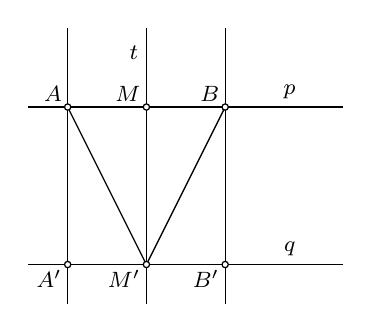
\begin{tikzpicture}
                    % \clip (0,0) rectangle (14.000000,10.000000);
                    {\footnotesize
                    
                    % Marking point A' by circle
                    \draw [line width=0.016cm] (2.000000,2.000000) circle (0.040000);%
                    \draw (2.030000,2.030000) node [anchor=north east] { $A'$ };%
                    
                    % Marking point A by circle
                    \draw [line width=0.016cm] (2.000000,4.000000) circle (0.040000);%
                    \draw (2.030000,3.970000) node [anchor=south east] { $A$ };%
                    
                    % Marking point B by circle
                    \draw [line width=0.016cm] (4.000000,4.000000) circle (0.040000);%
                    \draw (4.030000,3.970000) node [anchor=south east] { $B$ };%
                    
                    % Marking point B' by circle
                    \draw [line width=0.016cm] (4.000000,2.000000) circle (0.040000);%
                    \draw (4.030000,2.030000) node [anchor=north east] { $B'$ };%
                    
                    % Marking point M by circle
                    \draw [line width=0.016cm] (3.000000,4.000000) circle (0.040000);%
                    \draw (3.030000,3.970000) node [anchor=south east] { $M$ };%
                    
                    % Marking point M' by circle
                    \draw [line width=0.016cm] (3.000000,2.000000) circle (0.040000);%
                    \draw (3.030000,2.030000) node [anchor=north east] { $M'$ };%
                    
                    % Marking point p
                    \draw (5.000000,4.000000) node [anchor=south east] { $p$ };%
                    
                    % Marking point q
                    \draw (5.000000,2.000000) node [anchor=south east] { $q$ };%
                    
                    % Marking point t
                    \draw (3.000000,4.500000) node [anchor=south east] { $t$ };%
                    
                    % Drawing line P
                    \draw [line width=0.016cm] (1.500000,4.000000) -- (1.960000,4.000000);%
                    \draw [line width=0.016cm] (2.040000,4.000000) -- (2.960000,4.000000);%
                    \draw [line width=0.016cm] (3.040000,4.000000) -- (3.960000,4.000000);%
                    \draw [line width=0.016cm] (4.040000,4.000000) -- (5.500000,4.000000);%
                    
                    % Drawing line Q
                    \draw [line width=0.016cm] (1.500000,2.000000) -- (1.960000,2.000000);%
                    \draw [line width=0.016cm] (2.040000,2.000000) -- (2.960000,2.000000);%
                    \draw [line width=0.016cm] (3.040000,2.000000) -- (3.960000,2.000000);%
                    \draw [line width=0.016cm] (4.040000,2.000000) -- (5.500000,2.000000);%
                    
                    % Drawing line T
                    \draw [line width=0.016cm] (3.000000,1.500000) -- (3.000000,1.960000);%
                    \draw [line width=0.016cm] (3.000000,2.040000) -- (3.000000,3.960000);%
                    \draw [line width=0.016cm] (3.000000,4.040000) -- (3.000000,5.000000);%
                    
                    % Drawing line W
                    \draw [line width=0.016cm] (2.000000,1.500000) -- (2.000000,1.960000);%
                    \draw [line width=0.016cm] (2.000000,2.040000) -- (2.000000,3.960000);%
                    \draw [line width=0.016cm] (2.000000,4.040000) -- (2.000000,5.000000);%
                    
                    % Drawing line V
                    \draw [line width=0.016cm] (4.000000,1.500000) -- (4.000000,1.960000);%
                    \draw [line width=0.016cm] (4.000000,2.040000) -- (4.000000,3.960000);%
                    \draw [line width=0.016cm] (4.000000,4.040000) -- (4.000000,5.000000);%
                    
                    % Drawing segment A M'
                    \draw [line width=0.016cm] (2.017889,3.964223) -- (2.982111,2.035777);%
                    
                    % Drawing segment B M'
                    \draw [line width=0.016cm] (3.982111,3.964223) -- (3.017889,2.035777);%
                    }
                \end{tikzpicture}                
            \\ Po kriteriju SKS sledi, da sta trikotnika $\triangle M'A'A$ in $\triangle B'B'B$ skladna. Od tod sledi: $\angle A'M'A\cong \angle M'B'B$. Potem iz pravosti kotov $\angle MM'A'$ in $\angle MM'B'$ sledi: $\angle MM'A\cong \angle MM'B$. Po kriteriju SKS velja: $\triangle AMM' \cong \triangle BMM'$ (skupnna stranica $MM'$). Od tod sledi: $\angle AMM'\cong \angle AMM'$. Ker sta kota suplementarna, sta ta dva kota prava kota.
        \end{dokaz}

    \begin{lema}
        Če sta $p\parallel q$, imata lahko največ eno skupno pravokotnico.
    \end{lema}

        \begin{dokaz}
            Dve skupni pravokotnici, ki data pravokotnik, kar je protislovje (pravokotniki ne obstajajo).
        \end{dokaz}
    
    \begin{posledica}
        Naj bosta $p\parallel q$ in $A\in p$. Potem obstaja še največ ena druga točka na $p$, ki je od $q$ enako oddaljena kot $A$.
    \end{posledica}

        \begin{dokaz}
            \\ 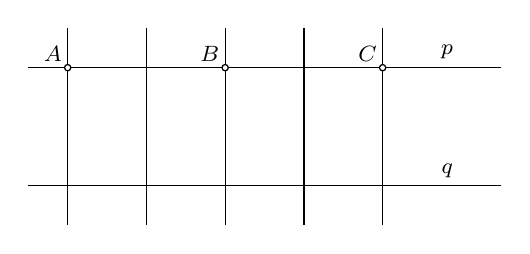
\begin{tikzpicture}
                    % \clip (0,0) rectangle (14.000000,10.000000);
                    {\footnotesize
                    
                    % Marking point C by circle
                    \draw [line width=0.016cm] (6.000000,4.000000) circle (0.040000);%
                    \draw (6.030000,3.970000) node [anchor=south east] { $C$ };%
                    
                    % Marking point A by circle
                    \draw [line width=0.016cm] (2.000000,4.000000) circle (0.040000);%
                    \draw (2.030000,3.970000) node [anchor=south east] { $A$ };%
                    
                    % Marking point B by circle
                    \draw [line width=0.016cm] (4.000000,4.000000) circle (0.040000);%
                    \draw (4.030000,3.970000) node [anchor=south east] { $B$ };%
                    
                    % Marking point p
                    \draw (7.000000,4.000000) node [anchor=south east] { $p$ };%
                    
                    % Marking point q
                    \draw (7.000000,2.500000) node [anchor=south east] { $q$ };%
                    
                    % Drawing line P
                    \draw [line width=0.016cm] (1.500000,4.000000) -- (1.960000,4.000000);%
                    \draw [line width=0.016cm] (2.040000,4.000000) -- (3.960000,4.000000);%
                    \draw [line width=0.016cm] (4.040000,4.000000) -- (5.960000,4.000000);%
                    \draw [line width=0.016cm] (6.040000,4.000000) -- (7.500000,4.000000);%
                    
                    % Drawing line Q
                    \draw [line width=0.016cm] (1.500000,2.500000) -- (7.500000,2.500000);%
                    
                    % Drawing line T
                    \draw [line width=0.016cm] (3.000000,2.000000) -- (3.000000,4.500000);%
                    
                    % Drawing line W
                    \draw [line width=0.016cm] (2.000000,2.000000) -- (2.000000,3.960000);%
                    \draw [line width=0.016cm] (2.000000,4.040000) -- (2.000000,4.500000);%
                    
                    % Drawing line V
                    \draw [line width=0.016cm] (4.000000,2.000000) -- (4.000000,3.960000);%
                    \draw [line width=0.016cm] (4.000000,4.040000) -- (4.000000,4.500000);%
                    
                    % Drawing line X
                    \draw [line width=0.016cm] (5.000000,2.000000) -- (5.000000,4.500000);%
                    
                    % Drawing line Y
                    \draw [line width=0.016cm] (6.000000,2.000000) -- (6.000000,3.960000);%
                    \draw [line width=0.016cm] (6.000000,4.040000) -- (6.000000,4.500000);%
                    }
                \end{tikzpicture}                
            \\ Če imamo primer kot na skici, potem bi $p$ in $q$ imeli dve skupni pravokotnici, kar je protislovje.
        \end{dokaz}

    \begin{posledica}
        Naj bosta $p\parallel q$ in naj imata $p$ in $q$ skupno pravokotnico $t$. Potem za vsak $A\in p$, ki ne leži na $t$ obstaja natanko ena točka $B\in p$ na nasprotnem bregu $t$ kot je $A$, ki je enako oddaljena od $q$ kot $A$.
    \end{posledica}

        % \begin{dokaz}
        %     ???
        % \end{dokaz}

    \begin{trditev}
        Naj bo $t$ skupna pravokotnica na vzporednici $p$ in $q$, ki seka ti dve premici v točkah $M$ in $M'$. Potem za poljubni točki $A,B\in p$, za kateri velja $M\ast A\ast B$, velja: $MM'<AA'<BB'$, kjer je $A'$ (oziroma $B'$) nožišče pravokotnice na $q$ skozi točko $A$ (oziroma $B$).
    \end{trditev}

        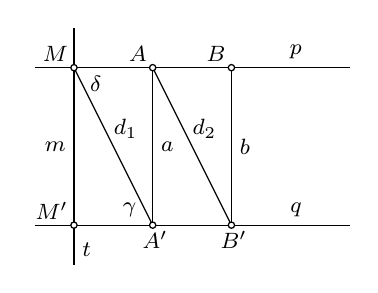
\begin{tikzpicture}
            % \clip (0,0) rectangle (14.000000,10.000000);
            {\footnotesize
            
            % Marking point A' by circle
            \draw [line width=0.016cm] (3.000000,2.000000) circle (0.040000);%
            \draw (3.030000,2.030000) node [anchor=north] { $A'$ };%
            
            % Marking point A by circle
            \draw [line width=0.016cm] (3.000000,4.000000) circle (0.040000);%
            \draw (3.030000,3.970000) node [anchor=south east] { $A$ };%
            
            % Marking point B by circle
            \draw [line width=0.016cm] (4.000000,4.000000) circle (0.040000);%
            \draw (4.030000,3.970000) node [anchor=south east] { $B$ };%
            
            % Marking point B' by circle
            \draw [line width=0.016cm] (4.000000,2.000000) circle (0.040000);%
            \draw (4.030000,2.030000) node [anchor=north] { $B'$ };%
            
            % Marking point M by circle
            \draw [line width=0.016cm] (2.000000,4.000000) circle (0.040000);%
            \draw (2.030000,3.970000) node [anchor=south east] { $M$ };%
            
            % Marking point M' by circle
            \draw [line width=0.016cm] (2.000000,2.000000) circle (0.040000);%
            \draw (2.030000,1.970000) node [anchor=south east] { $M'$ };%
            
            % Marking point p
            \draw (5.000000,4.000000) node [anchor=south east] { $p$ };%
            
            % Marking point q
            \draw (5.000000,2.000000) node [anchor=south east] { $q$ };%
            
            % Marking point t
            \draw (2.000000,1.500000) node [anchor=south west] { $t$ };%
            
            % Marking point m
            \draw (2.000000,3.000000) node [anchor=east] { $m$ };%
            
            % Marking point a
            \draw (3.000000,3.000000) node [anchor=west] { $a$ };%
            
            % Marking point b
            \draw (4.000000,3.000000) node [anchor=west] { $b$ };%
            
            % Marking point d_1
            \draw (2.400000,3.000000) node [anchor=south west] { $d_1$ };%
            
            % Marking point d_2
            \draw (3.400000,3.000000) node [anchor=south west] { $d_2$ };%
            
            % Marking point \delta
            \draw (2.100000,4.000000) node [anchor=north west] { $\delta$ };%
            
            % Marking point \gamma
            \draw (2.900000,2.000000) node [anchor=south east] { $\gamma$ };%
            
            % Drawing line P
            \draw [line width=0.016cm] (1.500000,4.000000) -- (1.960000,4.000000);%
            \draw [line width=0.016cm] (2.040000,4.000000) -- (2.960000,4.000000);%
            \draw [line width=0.016cm] (3.040000,4.000000) -- (3.960000,4.000000);%
            \draw [line width=0.016cm] (4.040000,4.000000) -- (5.500000,4.000000);%
            
            % Drawing line Q
            \draw [line width=0.016cm] (1.500000,2.000000) -- (1.960000,2.000000);%
            \draw [line width=0.016cm] (2.040000,2.000000) -- (2.960000,2.000000);%
            \draw [line width=0.016cm] (3.040000,2.000000) -- (3.960000,2.000000);%
            \draw [line width=0.016cm] (4.040000,2.000000) -- (5.500000,2.000000);%
            
            % Drawing line T
            \draw [line width=0.016cm] (2.000000,1.500000) -- (2.000000,1.960000);%
            \draw [line width=0.016cm] (2.000000,2.040000) -- (2.000000,3.960000);%
            \draw [line width=0.016cm] (2.000000,4.040000) -- (2.000000,4.500000);%
            
            % Drawing segment A' M
            \draw [line width=0.016cm] (2.982111,2.035777) -- (2.017889,3.964223);%
            
            % Drawing segment B' A
            \draw [line width=0.016cm] (3.982111,2.035777) -- (3.017889,3.964223);%
            
            % Drawing segment B B'
            \draw [line width=0.016cm] (4.000000,3.960000) -- (4.000000,2.040000);%
            
            % Drawing segment A A'
            \draw [line width=0.016cm] (3.000000,3.960000) -- (3.000000,2.040000);%
            }
        \end{tikzpicture}
        
        \begin{dokaz}
            \\ Dokazati moramo: \dashuline{$m<a<b$}.
            \\ 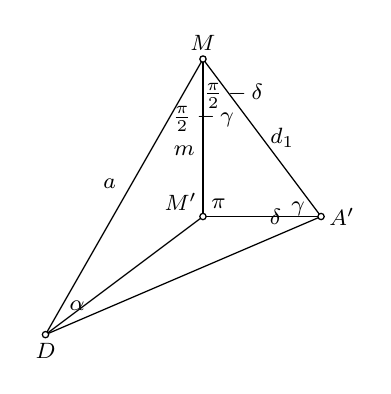
\begin{tikzpicture}
                    % \clip (0,0) rectangle (14.000000,10.000000);
                    {\footnotesize
                    
                    % Drawing segment D A'
                    \draw [line width=0.016cm] (2.036766,2.015757) -- (5.463234,3.484243);%
                    
                    % Drawing segment A' M
                    \draw [line width=0.016cm] (5.476000,3.532000) -- (4.024000,5.468000);%
                    
                    % Drawing segment M D
                    \draw [line width=0.016cm] (3.980154,5.465270) -- (2.019846,2.034730);%
                    
                    % Drawing segment D M'
                    \draw [line width=0.016cm] (2.032000,2.024000) -- (3.968000,3.476000);%
                    
                    % Drawing segment M' A'
                    \draw [line width=0.016cm] (4.040000,3.500000) -- (5.460000,3.500000);%
                    
                    % Drawing segment M M'
                    \draw [line width=0.016cm] (4.000000,5.460000) -- (4.000000,3.540000);%
                    
                    % Marking point D by circle
                    \draw [line width=0.016cm] (2.000000,2.000000) circle (0.040000);%
                    \draw (2.000000,2.000000) node [anchor=north] { $D$ };%
                    
                    % Marking point A' by circle
                    \draw [line width=0.016cm] (5.500000,3.500000) circle (0.040000);%
                    \draw (5.500000,3.500000) node [anchor=west] { $A'$ };%
                    
                    % Marking point M by circle
                    \draw [line width=0.016cm] (4.000000,5.500000) circle (0.040000);%
                    \draw (4.000000,5.500000) node [anchor=south] { $M$ };%
                    
                    % Marking point M' by circle
                    \draw [line width=0.016cm] (4.000000,3.500000) circle (0.040000);%
                    \draw (4.030000,3.470000) node [anchor=south east] { $M'$ };%
                    
                    % Marking point d_1
                    \draw (4.750000,4.500000) node [anchor=west] { $d_1$ };%
                    
                    % Marking point a
                    \draw (3.000000,3.750000) node [anchor=south east] { $a$ };%
                    
                    % Marking point m
                    \draw (4.000000,4.500000) node [anchor=north east] { $m$ };%
                    
                    % Marking point \alpha
                    \draw (2.200000,2.200000) node [anchor=south west] { $\alpha$ };%
                    
                    % Marking point \delta
                    \draw (5.100000,3.500000) node [anchor=east] { $\delta$ };%
                    
                    % Marking point \gamma
                    \draw (5.400000,3.400000) node [anchor=south east] { $\gamma$ };%
                    
                    % Marking point \frac{\pi}{2}-\gamma
                    \draw (4.000000,5.000000) node [anchor=north] { $\frac{\pi}{2}-\gamma$ };%
                    
                    % Marking point \frac{\pi}{2}-\delta
                    \draw (3.900000,5.300000) node [anchor=north west] { $\frac{\pi}{2}-\delta$ };%
                    
                    % Marking point \pi
                    \draw (4.000000,3.500000) node [anchor=south west] { $\pi$ };%
                    }
                \end{tikzpicture}
            \\ V trikotniku $\triangle MM'A'$ velja: $\frac{\pi}{2}+\gamma+\frac{\pi}{2}-\delta<\pi$, od koder sledi: $\gamma<\delta$ in $\frac{\pi}{2}-\gamma>\frac{\pi}{2}-\delta$. Iz skladnosti trikotnikov $\triangle A'MD\cong \triangle MA'A$ sledi $MD\cong AA'$ in od tod: $|MD|=a$. Zaradi vsote kotov v štirikotniku $\square MM'A'A$ je $|\angle D|=\alpha<\frac{\pi}{2}$. V trikotniku $\triangle MM'D$ je kot $|\angle D|=|\angle MDM'|=\alpha<\frac{\pi}{2}$ in $|\angle M'|=|\angle DM'M|>\frac{\pi}{2}$. Ker je večja stranica nasproti večjega kota v trikotniku, sledi $a>m$. Podobno sledi $a<b$.
        \end{dokaz}

    \begin{opomba}
        Zgornje obnašanje pomeni, da se vzporednici s skupno pravokotnico na obe strani oddaljujeta, zato ju imenujemo divergentni vzporednici.
        Še več, razdalja med takima vzporednicama gre v neskončnosti/$\infty$, ko potujemo po premici, v neskončnost/$\infty$.
        \\ Poleg tega obstaja še en tip vzporednic, ki pa se na eni strani asimptotično približujejo. Takim rečemo asimptotične vzporednice. 
    \end{opomba}

    \begin{izrek}
        Za premico $p$ in točko $A\notin p$ naj bo $B$ nožišče pravokotnice iz $A$ na $p$ ter naj bo premica $q$ pravokotnica na premico $\overleftrightarrow{AB}$ v točki $A$. Potem obstajata poltraka $\overrightarrow{AC}$ in $\overrightarrow{AC'}$, vsak na svojem bregu premice $\overleftrightarrow{AB}$, za katera velja:
        \begin{enumerate}
            \item $\overrightarrow{AC}$ in $\overrightarrow{AC'}$ ne sekata premice $p$;
            \item poltrak $\overrightarrow{AD}$ seka premico $p$ $\Leftrightarrow$ točka $D$ leži znotraj kota $\angle CAC'$;
            \item skladnost kotov: $\angle BAC\cong\angle BAC'$.
        \end{enumerate}
    \end{izrek}

        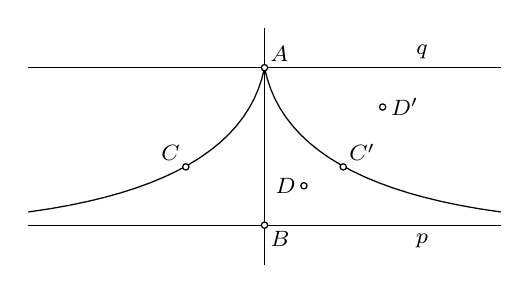
\begin{tikzpicture}
            % \clip (0,0) rectangle (14.000000,10.000000);
            {\footnotesize
            
            % Drawing line A B
            \draw [line width=0.016cm] (4.000000,1.500000) -- (4.000000,1.960000);%
            \draw [line width=0.016cm] (4.000000,2.040000) -- (4.000000,3.960000);%
            \draw [line width=0.016cm] (4.000000,4.040000) -- (4.000000,4.500000);%
            
            % Drawing line A q
            \draw [line width=0.016cm] (1.000000,4.000000) -- (3.960000,4.000000);%
            \draw [line width=0.016cm] (4.040000,4.000000) -- (7.000000,4.000000);%
            
            % Drawing line B p
            \draw [line width=0.016cm] (1.000000,2.000000) -- (3.960000,2.000000);%
            \draw [line width=0.016cm] (4.040000,2.000000) -- (7.000000,2.000000);%
            
            % Drawing Bezier curve A U X
            \draw [line width=0.016cm] (3.966821,3.863580) -- (3.990547,3.961133);%
            \draw [line width=0.016cm] (3.922840,3.732099) -- (3.966821,3.863580);%
            \draw [line width=0.016cm] (3.868056,3.605556) -- (3.922840,3.732099);%
            \draw [line width=0.016cm] (3.802469,3.483951) -- (3.868056,3.605556);%
            \draw [line width=0.016cm] (3.726080,3.367284) -- (3.802469,3.483951);%
            \draw [line width=0.016cm] (3.638889,3.255556) -- (3.726080,3.367284);%
            \draw [line width=0.016cm] (3.540895,3.148765) -- (3.638889,3.255556);%
            \draw [line width=0.016cm] (3.432099,3.046914) -- (3.540895,3.148765);%
            \draw [line width=0.016cm] (3.312500,2.950000) -- (3.432099,3.046914);%
            \draw [line width=0.016cm] (3.182099,2.858025) -- (3.312500,2.950000);%
            \draw [line width=0.016cm] (3.040895,2.770988) -- (3.182099,2.858025);%
            \draw [line width=0.016cm] (2.888889,2.688889) -- (2.961765,2.728249);%
            \draw [line width=0.016cm] (3.030792,2.765531) -- (3.040895,2.770988);%
            \draw [line width=0.016cm] (2.726080,2.611728) -- (2.888889,2.688889);%
            \draw [line width=0.016cm] (2.552469,2.539506) -- (2.726080,2.611728);%
            \draw [line width=0.016cm] (2.368056,2.472222) -- (2.552469,2.539506);%
            \draw [line width=0.016cm] (2.172840,2.409877) -- (2.368056,2.472222);%
            \draw [line width=0.016cm] (1.966821,2.352469) -- (2.172840,2.409877);%
            \draw [line width=0.016cm] (1.750000,2.300000) -- (1.966821,2.352469);%
            \draw [line width=0.016cm] (1.522377,2.252469) -- (1.750000,2.300000);%
            \draw [line width=0.016cm] (1.283951,2.209877) -- (1.522377,2.252469);%
            \draw [line width=0.016cm] (1.034722,2.172222) -- (1.283951,2.209877);%
            \draw [line width=0.016cm] (1.000000,2.167854) -- (1.034722,2.172222);%
            
            % Drawing Bezier curve A U' Y
            \draw [line width=0.016cm] (4.033179,3.863580) -- (4.009453,3.961133);%
            \draw [line width=0.016cm] (4.077160,3.732099) -- (4.033179,3.863580);%
            \draw [line width=0.016cm] (4.131944,3.605556) -- (4.077160,3.732099);%
            \draw [line width=0.016cm] (4.197531,3.483951) -- (4.131944,3.605556);%
            \draw [line width=0.016cm] (4.273920,3.367284) -- (4.197531,3.483951);%
            \draw [line width=0.016cm] (4.361111,3.255556) -- (4.273920,3.367284);%
            \draw [line width=0.016cm] (4.459105,3.148765) -- (4.361111,3.255556);%
            \draw [line width=0.016cm] (4.567901,3.046914) -- (4.459105,3.148765);%
            \draw [line width=0.016cm] (4.687500,2.950000) -- (4.567901,3.046914);%
            \draw [line width=0.016cm] (4.817901,2.858025) -- (4.687500,2.950000);%
            \draw [line width=0.016cm] (4.959105,2.770988) -- (4.817901,2.858025);%
            \draw [line width=0.016cm] (5.111111,2.688889) -- (5.038235,2.728249);%
            \draw [line width=0.016cm] (4.969208,2.765531) -- (4.959105,2.770988);%
            \draw [line width=0.016cm] (5.273920,2.611728) -- (5.111111,2.688889);%
            \draw [line width=0.016cm] (5.447531,2.539506) -- (5.273920,2.611728);%
            \draw [line width=0.016cm] (5.631944,2.472222) -- (5.447531,2.539506);%
            \draw [line width=0.016cm] (5.827160,2.409877) -- (5.631944,2.472222);%
            \draw [line width=0.016cm] (6.033179,2.352469) -- (5.827160,2.409877);%
            \draw [line width=0.016cm] (6.250000,2.300000) -- (6.033179,2.352469);%
            \draw [line width=0.016cm] (6.477623,2.252469) -- (6.250000,2.300000);%
            \draw [line width=0.016cm] (6.716049,2.209877) -- (6.477623,2.252469);%
            \draw [line width=0.016cm] (6.965278,2.172222) -- (6.716049,2.209877);%
            \draw [line width=0.016cm] (6.965278,2.172222) -- (7.000000,2.167854);%
            
            % Marking point A by circle
            \draw [line width=0.016cm] (4.000000,4.000000) circle (0.040000);%
            \draw (3.970000,3.970000) node [anchor=south west] { $A$ };%
            
            % Marking point B by circle
            \draw [line width=0.016cm] (4.000000,2.000000) circle (0.040000);%
            \draw (3.970000,2.030000) node [anchor=north west] { $B$ };%
            
            % Marking point p
            \draw (6.000000,2.000000) node [anchor=north] { $p$ };%
            
            % Marking point q
            \draw (6.000000,4.000000) node [anchor=south] { $q$ };%
            
            % Marking point C' by circle
            \draw [line width=0.016cm] (5.000000,2.740000) circle (0.040000);%
            \draw (4.970000,2.710000) node [anchor=south west] { $C'$ };%
            
            % Marking point C by circle
            \draw [line width=0.016cm] (3.000000,2.740000) circle (0.040000);%
            \draw (3.030000,2.710000) node [anchor=south east] { $C$ };%
            
            % Marking point D by circle
            \draw [line width=0.016cm] (4.500000,2.500000) circle (0.040000);%
            \draw (4.500000,2.500000) node [anchor=east] { $D$ };%
            
            % Marking point D' by circle
            \draw [line width=0.016cm] (5.500000,3.500000) circle (0.040000);%
            \draw (5.500000,3.500000) node [anchor=west] { $D'$ };%
            }
        \end{tikzpicture}
        
        \begin{dokaz}
            \\ Naj bo točka $E\in q$ na enem bregu premice $\overleftrightarrow{AB}$. Premico $\overleftrightarrow{BE}$ razdelimo na dve disjunktni podmnožici: $\Sigma_1=\{D\in BE | \overrightarrow{AD} ~seka~ p\}\cup \overrightarrow{BB'}$ in $\Sigma_2=\{D\in BE | \overrightarrow{AD} ~ne~seka~ p\}\cup \overrightarrow{EE'}$, in velja: $\Sigma_1\cup\Sigma_2=\overrightarrow{BE}$ in $\Sigma_1\cap\Sigma_2=\emptyset$.
            \\ 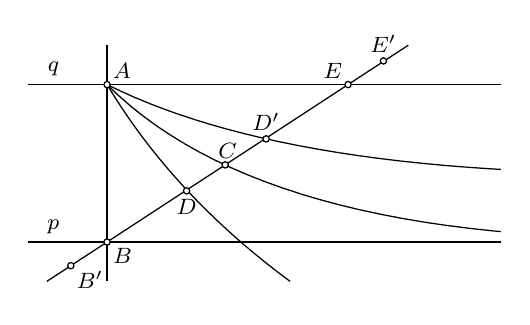
\begin{tikzpicture}
                    % \clip (0,0) rectangle (14.000000,10.000000);
                    {\footnotesize
                    
                    % Drawing line A B
                    \draw [line width=0.016cm] (2.000000,1.500000) -- (2.000000,1.960000);%
                    \draw [line width=0.016cm] (2.000000,2.040000) -- (2.000000,3.960000);%
                    \draw [line width=0.016cm] (2.000000,4.040000) -- (2.000000,4.500000);%
                    
                    % Drawing line A q
                    \draw [line width=0.016cm] (1.000000,4.000000) -- (1.960000,4.000000);%
                    \draw [line width=0.016cm] (2.040000,4.000000) -- (5.021224,4.000000);%
                    \draw [line width=0.016cm] (5.101224,4.000000) -- (7.000000,4.000000);%
                    
                    % Drawing line B p
                    \draw [line width=0.016cm] (1.000000,2.000000) -- (1.960000,2.000000);%
                    \draw [line width=0.016cm] (2.040000,2.000000) -- (7.000000,2.000000);%
                    
                    % Drawing line r
                    \draw [line width=0.016cm] (1.234694,1.500000) -- (1.506760,1.677750);%
                    \draw [line width=0.016cm] (1.573729,1.721503) -- (1.966513,1.978122);%
                    \draw [line width=0.016cm] (2.033487,2.021878) -- (2.972717,2.635509);%
                    \draw [line width=0.016cm] (3.038247,2.678321) -- (3.466513,2.958122);%
                    \draw [line width=0.016cm] (3.533487,3.001878) -- (3.982759,3.295402);%
                    \draw [line width=0.016cm] (4.048328,3.338241) -- (5.027738,3.978122);%
                    \draw [line width=0.016cm] (5.094711,4.021878) -- (5.479968,4.273579);%
                    \draw [line width=0.016cm] (5.546259,4.316889) -- (5.826531,4.500000);%
                    
                    % Drawing Bezier curve A U X
                    \draw [line width=0.016cm] (2.084877,3.861883) -- (2.020943,3.965921);%
                    \draw [line width=0.016cm] (2.172840,3.725309) -- (2.084877,3.861883);%
                    \draw [line width=0.016cm] (2.263889,3.590278) -- (2.172840,3.725309);%
                    \draw [line width=0.016cm] (2.358025,3.456790) -- (2.263889,3.590278);%
                    \draw [line width=0.016cm] (2.455247,3.324846) -- (2.358025,3.456790);%
                    \draw [line width=0.016cm] (2.555556,3.194444) -- (2.455247,3.324846);%
                    \draw [line width=0.016cm] (2.658951,3.065586) -- (2.555556,3.194444);%
                    \draw [line width=0.016cm] (2.765432,2.938272) -- (2.658951,3.065586);%
                    \draw [line width=0.016cm] (2.875000,2.812500) -- (2.765432,2.938272);%
                    \draw [line width=0.016cm] (2.987654,2.688272) -- (2.875000,2.812500);%
                    \draw [line width=0.016cm] (3.103395,2.565586) -- (3.043856,2.628698);%
                    \draw [line width=0.016cm] (2.990705,2.685038) -- (2.987654,2.688272);%
                    \draw [line width=0.016cm] (3.222222,2.444444) -- (3.103395,2.565586);%
                    \draw [line width=0.016cm] (3.344136,2.324846) -- (3.222222,2.444444);%
                    \draw [line width=0.016cm] (3.469136,2.206790) -- (3.344136,2.324846);%
                    \draw [line width=0.016cm] (3.597222,2.090278) -- (3.469136,2.206790);%
                    \draw [line width=0.016cm] (3.728395,1.975309) -- (3.597222,2.090278);%
                    \draw [line width=0.016cm] (3.862654,1.861883) -- (3.728395,1.975309);%
                    \draw [line width=0.016cm] (4.000000,1.750000) -- (3.862654,1.861883);%
                    \draw [line width=0.016cm] (4.140432,1.639660) -- (4.000000,1.750000);%
                    \draw [line width=0.016cm] (4.283951,1.530864) -- (4.140432,1.639660);%
                    \draw [line width=0.016cm] (4.326139,1.500000) -- (4.283951,1.530864);%
                    
                    % Drawing Bezier curve A U' Y
                    \draw [line width=0.016cm] (2.142747,3.863580) -- (2.028918,3.972364);%
                    \draw [line width=0.016cm] (2.293210,3.732099) -- (2.142747,3.863580);%
                    \draw [line width=0.016cm] (2.451389,3.605556) -- (2.293210,3.732099);%
                    \draw [line width=0.016cm] (2.617284,3.483951) -- (2.451389,3.605556);%
                    \draw [line width=0.016cm] (2.790895,3.367284) -- (2.617284,3.483951);%
                    \draw [line width=0.016cm] (2.972222,3.255556) -- (2.790895,3.367284);%
                    \draw [line width=0.016cm] (3.161265,3.148765) -- (2.972222,3.255556);%
                    \draw [line width=0.016cm] (3.358025,3.046914) -- (3.161265,3.148765);%
                    \draw [line width=0.016cm] (3.562500,2.950000) -- (3.535998,2.962561);%
                    \draw [line width=0.016cm] (3.463710,2.996823) -- (3.358025,3.046914);%
                    \draw [line width=0.016cm] (3.774691,2.858025) -- (3.562500,2.950000);%
                    \draw [line width=0.016cm] (3.994599,2.770988) -- (3.774691,2.858025);%
                    \draw [line width=0.016cm] (4.222222,2.688889) -- (3.994599,2.770988);%
                    \draw [line width=0.016cm] (4.457562,2.611728) -- (4.222222,2.688889);%
                    \draw [line width=0.016cm] (4.700617,2.539506) -- (4.457562,2.611728);%
                    \draw [line width=0.016cm] (4.951389,2.472222) -- (4.700617,2.539506);%
                    \draw [line width=0.016cm] (5.209877,2.409877) -- (4.951389,2.472222);%
                    \draw [line width=0.016cm] (5.476080,2.352469) -- (5.209877,2.409877);%
                    \draw [line width=0.016cm] (5.750000,2.300000) -- (5.476080,2.352469);%
                    \draw [line width=0.016cm] (6.031636,2.252469) -- (5.750000,2.300000);%
                    \draw [line width=0.016cm] (6.320988,2.209877) -- (6.031636,2.252469);%
                    \draw [line width=0.016cm] (6.618056,2.172222) -- (6.320988,2.209877);%
                    \draw [line width=0.016cm] (6.922840,2.139506) -- (6.618056,2.172222);%
                    \draw [line width=0.016cm] (6.922840,2.139506) -- (7.000000,2.132647);%
                    
                    % Drawing Bezier curve A U'' Z
                    \draw [line width=0.016cm] (2.169753,3.918210) -- (2.036035,3.982638);%
                    \draw [line width=0.016cm] (2.345679,3.839506) -- (2.169753,3.918210);%
                    \draw [line width=0.016cm] (2.527778,3.763889) -- (2.345679,3.839506);%
                    \draw [line width=0.016cm] (2.716049,3.691358) -- (2.527778,3.763889);%
                    \draw [line width=0.016cm] (2.910494,3.621914) -- (2.716049,3.691358);%
                    \draw [line width=0.016cm] (3.111111,3.555556) -- (2.910494,3.621914);%
                    \draw [line width=0.016cm] (3.317901,3.492284) -- (3.111111,3.555556);%
                    \draw [line width=0.016cm] (3.530864,3.432099) -- (3.317901,3.492284);%
                    \draw [line width=0.016cm] (3.750000,3.375000) -- (3.530864,3.432099);%
                    \draw [line width=0.016cm] (3.975309,3.320988) -- (3.750000,3.375000);%
                    \draw [line width=0.016cm] (4.206790,3.270062) -- (4.059293,3.302511);%
                    \draw [line width=0.016cm] (3.981192,3.319693) -- (3.975309,3.320988);%
                    \draw [line width=0.016cm] (4.444444,3.222222) -- (4.206790,3.270062);%
                    \draw [line width=0.016cm] (4.688272,3.177469) -- (4.444444,3.222222);%
                    \draw [line width=0.016cm] (4.938272,3.135802) -- (4.688272,3.177469);%
                    \draw [line width=0.016cm] (5.194444,3.097222) -- (4.938272,3.135802);%
                    \draw [line width=0.016cm] (5.456790,3.061728) -- (5.194444,3.097222);%
                    \draw [line width=0.016cm] (5.725309,3.029321) -- (5.456790,3.061728);%
                    \draw [line width=0.016cm] (6.000000,3.000000) -- (5.725309,3.029321);%
                    \draw [line width=0.016cm] (6.280864,2.973765) -- (6.000000,3.000000);%
                    \draw [line width=0.016cm] (6.567901,2.950617) -- (6.280864,2.973765);%
                    \draw [line width=0.016cm] (6.861111,2.930556) -- (6.567901,2.950617);%
                    \draw [line width=0.016cm] (6.861111,2.930556) -- (7.000000,2.922680);%
                    
                    % Marking point A by circle
                    \draw [line width=0.016cm] (2.000000,4.000000) circle (0.040000);%
                    \draw (1.970000,3.970000) node [anchor=south west] { $A$ };%
                    
                    % Marking point B by circle
                    \draw [line width=0.016cm] (2.000000,2.000000) circle (0.040000);%
                    \draw (1.970000,2.030000) node [anchor=north west] { $B$ };%
                    
                    % Marking point p
                    \draw (1.500000,2.000000) node [anchor=south east] { $p$ };%
                    
                    % Marking point q
                    \draw (1.500000,4.000000) node [anchor=south east] { $q$ };%
                    
                    % Marking point C by circle
                    \draw [line width=0.016cm] (3.500000,2.980000) circle (0.040000);%
                    \draw (3.530000,2.950000) node [anchor=south] { $C$ };%
                    
                    % Marking point D by circle
                    \draw [line width=0.016cm] (3.010000,2.650000) circle (0.040000);%
                    \draw (3.010000,2.650000) node [anchor=north] { $D$ };%
                    
                    % Marking point D' by circle
                    \draw [line width=0.016cm] (4.020000,3.310000) circle (0.040000);%
                    \draw (4.020000,3.310000) node [anchor=south] { $D'$ };%
                    
                    % Marking point E by circle
                    \draw [line width=0.016cm] (5.061224,4.000000) circle (0.040000);%
                    \draw (5.091224,3.970000) node [anchor=south east] { $E$ };%
                    
                    % Marking point B' by circle
                    \draw [line width=0.016cm] (1.540000,1.700000) circle (0.040000);%
                    \draw (1.510000,1.730000) node [anchor=north west] { $B'$ };%
                    
                    % Marking point E' by circle
                    \draw [line width=0.016cm] (5.510000,4.300000) circle (0.040000);%
                    \draw (5.510000,4.300000) node [anchor=south] { $E'$ };%
                    }
                \end{tikzpicture}                
            \\ Preveriti moramo, da nobena točka iz $\Sigma_1$ (oziroma $\Sigma_2$) ni med nobenima dvema točkama iz $\Sigma_1$ (oziroma $\Sigma_1$). 
            \\ 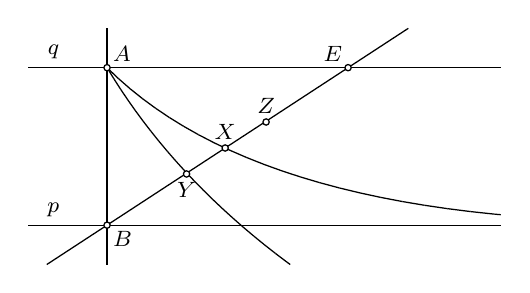
\begin{tikzpicture}
                    % \clip (0,0) rectangle (14.000000,10.000000);
                    {\footnotesize
                    
                    % Drawing line A B
                    \draw [line width=0.016cm] (2.000000,1.500000) -- (2.000000,1.960000);%
                    \draw [line width=0.016cm] (2.000000,2.040000) -- (2.000000,3.960000);%
                    \draw [line width=0.016cm] (2.000000,4.040000) -- (2.000000,4.500000);%
                    
                    % Drawing line A q
                    \draw [line width=0.016cm] (1.000000,4.000000) -- (1.960000,4.000000);%
                    \draw [line width=0.016cm] (2.040000,4.000000) -- (5.021224,4.000000);%
                    \draw [line width=0.016cm] (5.101224,4.000000) -- (7.000000,4.000000);%
                    
                    % Drawing line B p
                    \draw [line width=0.016cm] (1.000000,2.000000) -- (1.960000,2.000000);%
                    \draw [line width=0.016cm] (2.040000,2.000000) -- (7.000000,2.000000);%
                    
                    % Drawing line r
                    \draw [line width=0.016cm] (1.234694,1.500000) -- (1.966513,1.978122);%
                    \draw [line width=0.016cm] (2.033487,2.021878) -- (2.972717,2.635509);%
                    \draw [line width=0.016cm] (3.038247,2.678321) -- (3.466513,2.958122);%
                    \draw [line width=0.016cm] (3.533487,3.001878) -- (3.982759,3.295402);%
                    \draw [line width=0.016cm] (4.048328,3.338241) -- (5.027738,3.978122);%
                    \draw [line width=0.016cm] (5.094711,4.021878) -- (5.826531,4.500000);%
                    
                    % Drawing Bezier curve A U X'
                    \draw [line width=0.016cm] (2.084877,3.861883) -- (2.020943,3.965921);%
                    \draw [line width=0.016cm] (2.172840,3.725309) -- (2.084877,3.861883);%
                    \draw [line width=0.016cm] (2.263889,3.590278) -- (2.172840,3.725309);%
                    \draw [line width=0.016cm] (2.358025,3.456790) -- (2.263889,3.590278);%
                    \draw [line width=0.016cm] (2.455247,3.324846) -- (2.358025,3.456790);%
                    \draw [line width=0.016cm] (2.555556,3.194444) -- (2.455247,3.324846);%
                    \draw [line width=0.016cm] (2.658951,3.065586) -- (2.555556,3.194444);%
                    \draw [line width=0.016cm] (2.765432,2.938272) -- (2.658951,3.065586);%
                    \draw [line width=0.016cm] (2.875000,2.812500) -- (2.765432,2.938272);%
                    \draw [line width=0.016cm] (2.987654,2.688272) -- (2.875000,2.812500);%
                    \draw [line width=0.016cm] (3.103395,2.565586) -- (3.043856,2.628698);%
                    \draw [line width=0.016cm] (2.990705,2.685038) -- (2.987654,2.688272);%
                    \draw [line width=0.016cm] (3.222222,2.444444) -- (3.103395,2.565586);%
                    \draw [line width=0.016cm] (3.344136,2.324846) -- (3.222222,2.444444);%
                    \draw [line width=0.016cm] (3.469136,2.206790) -- (3.344136,2.324846);%
                    \draw [line width=0.016cm] (3.597222,2.090278) -- (3.469136,2.206790);%
                    \draw [line width=0.016cm] (3.728395,1.975309) -- (3.597222,2.090278);%
                    \draw [line width=0.016cm] (3.862654,1.861883) -- (3.728395,1.975309);%
                    \draw [line width=0.016cm] (4.000000,1.750000) -- (3.862654,1.861883);%
                    \draw [line width=0.016cm] (4.140432,1.639660) -- (4.000000,1.750000);%
                    \draw [line width=0.016cm] (4.283951,1.530864) -- (4.140432,1.639660);%
                    \draw [line width=0.016cm] (4.326139,1.500000) -- (4.283951,1.530864);%
                    
                    % Drawing Bezier curve A U' Y'
                    \draw [line width=0.016cm] (2.142747,3.863580) -- (2.028918,3.972364);%
                    \draw [line width=0.016cm] (2.293210,3.732099) -- (2.142747,3.863580);%
                    \draw [line width=0.016cm] (2.451389,3.605556) -- (2.293210,3.732099);%
                    \draw [line width=0.016cm] (2.617284,3.483951) -- (2.451389,3.605556);%
                    \draw [line width=0.016cm] (2.790895,3.367284) -- (2.617284,3.483951);%
                    \draw [line width=0.016cm] (2.972222,3.255556) -- (2.790895,3.367284);%
                    \draw [line width=0.016cm] (3.161265,3.148765) -- (2.972222,3.255556);%
                    \draw [line width=0.016cm] (3.358025,3.046914) -- (3.161265,3.148765);%
                    \draw [line width=0.016cm] (3.562500,2.950000) -- (3.535998,2.962561);%
                    \draw [line width=0.016cm] (3.463710,2.996823) -- (3.358025,3.046914);%
                    \draw [line width=0.016cm] (3.774691,2.858025) -- (3.562500,2.950000);%
                    \draw [line width=0.016cm] (3.994599,2.770988) -- (3.774691,2.858025);%
                    \draw [line width=0.016cm] (4.222222,2.688889) -- (3.994599,2.770988);%
                    \draw [line width=0.016cm] (4.457562,2.611728) -- (4.222222,2.688889);%
                    \draw [line width=0.016cm] (4.700617,2.539506) -- (4.457562,2.611728);%
                    \draw [line width=0.016cm] (4.951389,2.472222) -- (4.700617,2.539506);%
                    \draw [line width=0.016cm] (5.209877,2.409877) -- (4.951389,2.472222);%
                    \draw [line width=0.016cm] (5.476080,2.352469) -- (5.209877,2.409877);%
                    \draw [line width=0.016cm] (5.750000,2.300000) -- (5.476080,2.352469);%
                    \draw [line width=0.016cm] (6.031636,2.252469) -- (5.750000,2.300000);%
                    \draw [line width=0.016cm] (6.320988,2.209877) -- (6.031636,2.252469);%
                    \draw [line width=0.016cm] (6.618056,2.172222) -- (6.320988,2.209877);%
                    \draw [line width=0.016cm] (6.922840,2.139506) -- (6.618056,2.172222);%
                    \draw [line width=0.016cm] (6.922840,2.139506) -- (7.000000,2.132647);%
                    
                    % Marking point A by circle
                    \draw [line width=0.016cm] (2.000000,4.000000) circle (0.040000);%
                    \draw (1.970000,3.970000) node [anchor=south west] { $A$ };%
                    
                    % Marking point B by circle
                    \draw [line width=0.016cm] (2.000000,2.000000) circle (0.040000);%
                    \draw (1.970000,2.030000) node [anchor=north west] { $B$ };%
                    
                    % Marking point p
                    \draw (1.500000,2.000000) node [anchor=south east] { $p$ };%
                    
                    % Marking point q
                    \draw (1.500000,4.000000) node [anchor=south east] { $q$ };%
                    
                    % Marking point X by circle
                    \draw [line width=0.016cm] (3.500000,2.980000) circle (0.040000);%
                    \draw (3.500000,2.980000) node [anchor=south] { $X$ };%
                    
                    % Marking point Y by circle
                    \draw [line width=0.016cm] (3.010000,2.650000) circle (0.040000);%
                    \draw (3.010000,2.650000) node [anchor=north] { $Y$ };%
                    
                    % Marking point Z by circle
                    \draw [line width=0.016cm] (4.020000,3.310000) circle (0.040000);%
                    \draw (4.020000,3.310000) node [anchor=south] { $Z$ };%
                    
                    % Marking point E by circle
                    \draw [line width=0.016cm] (5.061224,4.000000) circle (0.040000);%
                    \draw (5.091224,3.970000) node [anchor=south east] { $E$ };%
                    }
                \end{tikzpicture}                
            \\ Če je $X\in\Sigma_1$, $Y\ast X\ast Z; Y,Z\in\Sigma_2$ za $X,Y,Z\in\overrightarrow{BE}$, potem bi $\overrightarrow{AY}$ (oziroma $\overrightarrow{AZ}$) po izreku o prečnici sekal premico $p$. To pa je v protislovju z $Y\in\Sigma_2$. 
            \\ 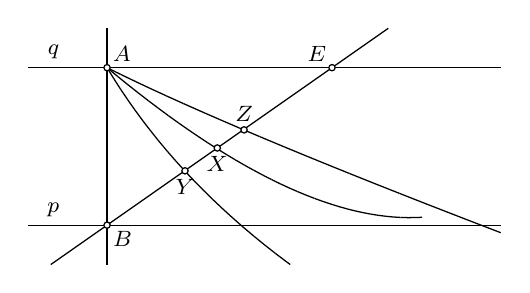
\begin{tikzpicture}
                    % \clip (0,0) rectangle (14.000000,10.000000);
                    {\footnotesize
                    
                    % Drawing line A B
                    \draw [line width=0.016cm] (2.000000,1.500000) -- (2.000000,1.960000);%
                    \draw [line width=0.016cm] (2.000000,2.040000) -- (2.000000,3.960000);%
                    \draw [line width=0.016cm] (2.000000,4.040000) -- (2.000000,4.500000);%
                    
                    % Drawing line A q
                    \draw [line width=0.016cm] (1.000000,4.000000) -- (1.960000,4.000000);%
                    \draw [line width=0.016cm] (2.040000,4.000000) -- (4.817143,4.000000);%
                    \draw [line width=0.016cm] (4.897143,4.000000) -- (7.000000,4.000000);%
                    
                    % Drawing line B p
                    \draw [line width=0.016cm] (1.000000,2.000000) -- (1.960000,2.000000);%
                    \draw [line width=0.016cm] (2.040000,2.000000) -- (7.000000,2.000000);%
                    
                    % Drawing line r
                    \draw [line width=0.016cm] (1.285714,1.500000) -- (1.967231,1.977062);%
                    \draw [line width=0.016cm] (2.032769,2.022938) -- (2.955883,2.669118);%
                    \draw [line width=0.016cm] (3.021298,2.714909) -- (3.367231,2.957062);%
                    \draw [line width=0.016cm] (3.432769,3.002938) -- (3.703915,3.192741);%
                    \draw [line width=0.016cm] (3.768568,3.237998) -- (4.824374,3.977062);%
                    \draw [line width=0.016cm] (4.889912,4.022938) -- (5.571429,4.500000);%
                    
                    % Drawing Bezier curve A U X'
                    \draw [line width=0.016cm] (2.084877,3.861883) -- (2.020943,3.965921);%
                    \draw [line width=0.016cm] (2.172840,3.725309) -- (2.084877,3.861883);%
                    \draw [line width=0.016cm] (2.263889,3.590278) -- (2.172840,3.725309);%
                    \draw [line width=0.016cm] (2.358025,3.456790) -- (2.263889,3.590278);%
                    \draw [line width=0.016cm] (2.455247,3.324846) -- (2.358025,3.456790);%
                    \draw [line width=0.016cm] (2.555556,3.194444) -- (2.455247,3.324846);%
                    \draw [line width=0.016cm] (2.658951,3.065586) -- (2.555556,3.194444);%
                    \draw [line width=0.016cm] (2.765432,2.938272) -- (2.658951,3.065586);%
                    \draw [line width=0.016cm] (2.875000,2.812500) -- (2.765432,2.938272);%
                    \draw [line width=0.016cm] (2.961053,2.717606) -- (2.875000,2.812500);%
                    \draw [line width=0.016cm] (3.103395,2.565586) -- (3.015273,2.658996);%
                    \draw [line width=0.016cm] (3.222222,2.444444) -- (3.103395,2.565586);%
                    \draw [line width=0.016cm] (3.344136,2.324846) -- (3.222222,2.444444);%
                    \draw [line width=0.016cm] (3.469136,2.206790) -- (3.344136,2.324846);%
                    \draw [line width=0.016cm] (3.597222,2.090278) -- (3.469136,2.206790);%
                    \draw [line width=0.016cm] (3.728395,1.975309) -- (3.597222,2.090278);%
                    \draw [line width=0.016cm] (3.862654,1.861883) -- (3.728395,1.975309);%
                    \draw [line width=0.016cm] (4.000000,1.750000) -- (3.862654,1.861883);%
                    \draw [line width=0.016cm] (4.140432,1.639660) -- (4.000000,1.750000);%
                    \draw [line width=0.016cm] (4.283951,1.530864) -- (4.140432,1.639660);%
                    \draw [line width=0.016cm] (4.326139,1.500000) -- (4.283951,1.530864);%
                    
                    % Drawing Bezier curve A U' Y'
                    \draw [line width=0.016cm] (2.132716,3.890509) -- (2.030855,3.974545);%
                    \draw [line width=0.016cm] (2.264198,3.784259) -- (2.132716,3.890509);%
                    \draw [line width=0.016cm] (2.394444,3.681250) -- (2.264198,3.784259);%
                    \draw [line width=0.016cm] (2.523457,3.581481) -- (2.394444,3.681250);%
                    \draw [line width=0.016cm] (2.651235,3.484954) -- (2.523457,3.581481);%
                    \draw [line width=0.016cm] (2.777778,3.391667) -- (2.651235,3.484954);%
                    \draw [line width=0.016cm] (2.903086,3.301620) -- (2.777778,3.391667);%
                    \draw [line width=0.016cm] (3.027160,3.214815) -- (2.903086,3.301620);%
                    \draw [line width=0.016cm] (3.150000,3.131250) -- (3.027160,3.214815);%
                    \draw [line width=0.016cm] (3.271605,3.050926) -- (3.150000,3.131250);%
                    \draw [line width=0.016cm] (3.362151,2.992941) -- (3.271605,3.050926);%
                    \draw [line width=0.016cm] (3.511111,2.900000) -- (3.428050,2.951483);%
                    \draw [line width=0.016cm] (3.629012,2.829398) -- (3.511111,2.900000);%
                    \draw [line width=0.016cm] (3.745679,2.762037) -- (3.629012,2.829398);%
                    \draw [line width=0.016cm] (3.861111,2.697917) -- (3.745679,2.762037);%
                    \draw [line width=0.016cm] (3.975309,2.637037) -- (3.861111,2.697917);%
                    \draw [line width=0.016cm] (4.088272,2.579398) -- (3.975309,2.637037);%
                    \draw [line width=0.016cm] (4.200000,2.525000) -- (4.088272,2.579398);%
                    \draw [line width=0.016cm] (4.310494,2.473843) -- (4.200000,2.525000);%
                    \draw [line width=0.016cm] (4.419753,2.425926) -- (4.310494,2.473843);%
                    \draw [line width=0.016cm] (4.527778,2.381250) -- (4.419753,2.425926);%
                    \draw [line width=0.016cm] (4.634568,2.339815) -- (4.527778,2.381250);%
                    \draw [line width=0.016cm] (4.740123,2.301620) -- (4.634568,2.339815);%
                    \draw [line width=0.016cm] (4.844444,2.266667) -- (4.740123,2.301620);%
                    \draw [line width=0.016cm] (4.947531,2.234954) -- (4.844444,2.266667);%
                    \draw [line width=0.016cm] (5.049383,2.206481) -- (4.947531,2.234954);%
                    \draw [line width=0.016cm] (5.150000,2.181250) -- (5.049383,2.206481);%
                    \draw [line width=0.016cm] (5.249383,2.159259) -- (5.150000,2.181250);%
                    \draw [line width=0.016cm] (5.347531,2.140509) -- (5.249383,2.159259);%
                    \draw [line width=0.016cm] (5.444444,2.125000) -- (5.347531,2.140509);%
                    \draw [line width=0.016cm] (5.540123,2.112731) -- (5.444444,2.125000);%
                    \draw [line width=0.016cm] (5.634568,2.103704) -- (5.540123,2.112731);%
                    \draw [line width=0.016cm] (5.727778,2.097917) -- (5.634568,2.103704);%
                    \draw [line width=0.016cm] (5.819753,2.095370) -- (5.727778,2.097917);%
                    \draw [line width=0.016cm] (5.910494,2.096065) -- (5.819753,2.095370);%
                    \draw [line width=0.016cm] (6.000000,2.100000) -- (5.910494,2.096065);%
                    
                    % Drawing Bezier curve A U'' Z'
                    \draw [line width=0.016cm] (2.172068,3.915123) -- (2.035873,3.982305);%
                    \draw [line width=0.016cm] (2.354938,3.827160) -- (2.172068,3.915123);%
                    \draw [line width=0.016cm] (2.548611,3.736111) -- (2.354938,3.827160);%
                    \draw [line width=0.016cm] (2.753086,3.641975) -- (2.548611,3.736111);%
                    \draw [line width=0.016cm] (2.968364,3.544753) -- (2.753086,3.641975);%
                    \draw [line width=0.016cm] (3.194444,3.444444) -- (2.968364,3.544753);%
                    \draw [line width=0.016cm] (3.431327,3.341049) -- (3.194444,3.444444);%
                    \draw [line width=0.016cm] (3.679012,3.234568) -- (3.431327,3.341049);%
                    \draw [line width=0.016cm] (3.937500,3.125000) -- (3.776351,3.193308);%
                    \draw [line width=0.016cm] (3.702727,3.224516) -- (3.679012,3.234568);%
                    \draw [line width=0.016cm] (4.206790,3.012346) -- (3.937500,3.125000);%
                    \draw [line width=0.016cm] (4.486883,2.896605) -- (4.206790,3.012346);%
                    \draw [line width=0.016cm] (4.777778,2.777778) -- (4.486883,2.896605);%
                    \draw [line width=0.016cm] (5.079475,2.655864) -- (4.777778,2.777778);%
                    \draw [line width=0.016cm] (5.391975,2.530864) -- (5.079475,2.655864);%
                    \draw [line width=0.016cm] (5.715278,2.402778) -- (5.391975,2.530864);%
                    \draw [line width=0.016cm] (6.049383,2.271605) -- (5.715278,2.402778);%
                    \draw [line width=0.016cm] (6.394290,2.137346) -- (6.049383,2.271605);%
                    \draw [line width=0.016cm] (6.750000,2.000000) -- (6.394290,2.137346);%
                    \draw [line width=0.016cm] (6.750000,2.000000) -- (7.000000,1.904211);%
                    
                    % Marking point A by circle
                    \draw [line width=0.016cm] (2.000000,4.000000) circle (0.040000);%
                    \draw (1.970000,3.970000) node [anchor=south west] { $A$ };%
                    
                    % Marking point B by circle
                    \draw [line width=0.016cm] (2.000000,2.000000) circle (0.040000);%
                    \draw (1.970000,2.030000) node [anchor=north west] { $B$ };%
                    
                    % Marking point p
                    \draw (1.500000,2.000000) node [anchor=south east] { $p$ };%
                    
                    % Marking point q
                    \draw (1.500000,4.000000) node [anchor=south east] { $q$ };%
                    
                    % Marking point X by circle
                    \draw [line width=0.016cm] (3.400000,2.980000) circle (0.040000);%
                    \draw (3.400000,2.980000) node [anchor=north] { $X$ };%
                    
                    % Marking point Y by circle
                    \draw [line width=0.016cm] (2.990000,2.690000) circle (0.040000);%
                    \draw (2.990000,2.690000) node [anchor=north] { $Y$ };%
                    
                    % Marking point Z by circle
                    \draw [line width=0.016cm] (3.740000,3.210000) circle (0.040000);%
                    \draw (3.740000,3.210000) node [anchor=south] { $Z$ };%
                    
                    % Marking point E by circle
                    \draw [line width=0.016cm] (4.857143,4.000000) circle (0.040000);%
                    \draw (4.887143,3.970000) node [anchor=south east] { $E$ };%
                    }
                \end{tikzpicture}                
            \\ Če je $X\in\Sigma_2$, $Y\ast X\ast Z; Y,Z\in\Sigma_1$ za $X,Y,Z\in\overrightarrow{BE}$, potem bi $\overrightarrow{AX}$ sekal premico $p$. To pa je v protislovju z $X\in\Sigma_2$. Potem po Dedekindovem aksiomu obstaja natanko ena točka $C\in BE$, ki razdeli poltrak $\overrightarrow{BE}$ na množiči $\Sigma_1$ in $\Sigma_2$.
            \\ Da dokažemo točki (1) in (2), moramo preveriti \dashuline{$C\in\Sigma_2$}. 
            \\ 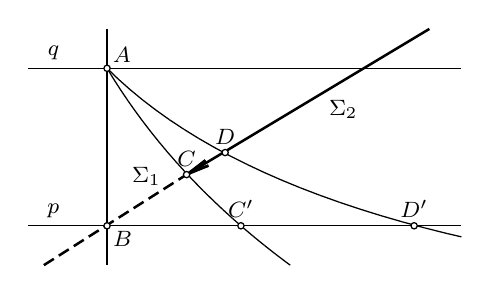
\begin{tikzpicture}
                    % \clip (0,0) rectangle (14.000000,10.000000);
                    {\footnotesize
                    
                    % Drawing line A B
                    \draw [line width=0.016cm] (2.000000,1.500000) -- (2.000000,1.960000);%
                    \draw [line width=0.016cm] (2.000000,2.040000) -- (2.000000,3.960000);%
                    \draw [line width=0.016cm] (2.000000,4.040000) -- (2.000000,4.500000);%
                    
                    % Drawing line A q
                    \draw [line width=0.016cm] (1.000000,4.000000) -- (1.960000,4.000000);%
                    \draw [line width=0.016cm] (2.040000,4.000000) -- (6.500000,4.000000);%
                    
                    % Drawing line B p
                    \draw [line width=0.016cm] (1.000000,2.000000) -- (1.960000,2.000000);%
                    \draw [line width=0.016cm] (2.040000,2.000000) -- (3.660000,2.000000);%
                    \draw [line width=0.016cm] (3.740000,2.000000) -- (5.860000,2.000000);%
                    \draw [line width=0.016cm] (5.940000,2.000000) -- (6.500000,2.000000);%
                    
                    % Drawing Bezier curve A U X
                    \draw [line width=0.016cm] (2.084877,3.861883) -- (2.020943,3.965921);%
                    \draw [line width=0.016cm] (2.172840,3.725309) -- (2.084877,3.861883);%
                    \draw [line width=0.016cm] (2.263889,3.590278) -- (2.172840,3.725309);%
                    \draw [line width=0.016cm] (2.358025,3.456790) -- (2.263889,3.590278);%
                    \draw [line width=0.016cm] (2.455247,3.324846) -- (2.358025,3.456790);%
                    \draw [line width=0.016cm] (2.555556,3.194444) -- (2.455247,3.324846);%
                    \draw [line width=0.016cm] (2.658951,3.065586) -- (2.555556,3.194444);%
                    \draw [line width=0.016cm] (2.765432,2.938272) -- (2.658951,3.065586);%
                    \draw [line width=0.016cm] (2.875000,2.812500) -- (2.765432,2.938272);%
                    \draw [line width=0.016cm] (2.987654,2.688272) -- (2.875000,2.812500);%
                    \draw [line width=0.016cm] (3.103395,2.565586) -- (3.043856,2.628698);%
                    \draw [line width=0.016cm] (2.990705,2.685038) -- (2.987654,2.688272);%
                    \draw [line width=0.016cm] (3.222222,2.444444) -- (3.103395,2.565586);%
                    \draw [line width=0.016cm] (3.344136,2.324846) -- (3.222222,2.444444);%
                    \draw [line width=0.016cm] (3.469136,2.206790) -- (3.344136,2.324846);%
                    \draw [line width=0.016cm] (3.597222,2.090278) -- (3.469136,2.206790);%
                    \draw [line width=0.016cm] (3.670016,2.026476) -- (3.597222,2.090278);%
                    \draw [line width=0.016cm] (3.862654,1.861883) -- (3.730206,1.973778);%
                    \draw [line width=0.016cm] (4.000000,1.750000) -- (3.862654,1.861883);%
                    \draw [line width=0.016cm] (4.140432,1.639660) -- (4.000000,1.750000);%
                    \draw [line width=0.016cm] (4.283951,1.530864) -- (4.140432,1.639660);%
                    \draw [line width=0.016cm] (4.326139,1.500000) -- (4.283951,1.530864);%
                    
                    % Drawing Bezier curve A U' Y
                    \draw [line width=0.016cm] (2.142747,3.862809) -- (2.028840,3.972283);%
                    \draw [line width=0.016cm] (2.293210,3.729012) -- (2.142747,3.862809);%
                    \draw [line width=0.016cm] (2.451389,3.598611) -- (2.293210,3.729012);%
                    \draw [line width=0.016cm] (2.617284,3.471605) -- (2.451389,3.598611);%
                    \draw [line width=0.016cm] (2.790895,3.347994) -- (2.617284,3.471605);%
                    \draw [line width=0.016cm] (2.972222,3.227778) -- (2.790895,3.347994);%
                    \draw [line width=0.016cm] (3.161265,3.110957) -- (2.972222,3.227778);%
                    \draw [line width=0.016cm] (3.358025,2.997531) -- (3.161265,3.110957);%
                    \draw [line width=0.016cm] (3.562500,2.887500) -- (3.530846,2.904534);%
                    \draw [line width=0.016cm] (3.461753,2.941713) -- (3.358025,2.997531);%
                    \draw [line width=0.016cm] (3.774691,2.780864) -- (3.562500,2.887500);%
                    \draw [line width=0.016cm] (3.994599,2.677623) -- (3.774691,2.780864);%
                    \draw [line width=0.016cm] (4.222222,2.577778) -- (3.994599,2.677623);%
                    \draw [line width=0.016cm] (4.457562,2.481327) -- (4.222222,2.577778);%
                    \draw [line width=0.016cm] (4.700617,2.388272) -- (4.457562,2.481327);%
                    \draw [line width=0.016cm] (4.951389,2.298611) -- (4.700617,2.388272);%
                    \draw [line width=0.016cm] (5.209877,2.212346) -- (4.951389,2.298611);%
                    \draw [line width=0.016cm] (5.476080,2.129475) -- (5.209877,2.212346);%
                    \draw [line width=0.016cm] (5.750000,2.050000) -- (5.476080,2.129475);%
                    \draw [line width=0.016cm] (6.031636,1.973920) -- (5.939978,1.998680);%
                    \draw [line width=0.016cm] (5.864795,2.018990) -- (5.750000,2.050000);%
                    \draw [line width=0.016cm] (6.320988,1.901235) -- (6.031636,1.973920);%
                    \draw [line width=0.016cm] (6.320988,1.901235) -- (6.500000,1.859481);%
                    
                    % Marking point A by circle
                    \draw [line width=0.016cm] (2.000000,4.000000) circle (0.040000);%
                    \draw (1.970000,3.970000) node [anchor=south west] { $A$ };%
                    
                    % Marking point B by circle
                    \draw [line width=0.016cm] (2.000000,2.000000) circle (0.040000);%
                    \draw (1.970000,2.030000) node [anchor=north west] { $B$ };%
                    
                    % Marking point p
                    \draw (1.500000,2.000000) node [anchor=south east] { $p$ };%
                    
                    % Marking point q
                    \draw (1.500000,4.000000) node [anchor=south east] { $q$ };%
                    
                    % Marking point D by circle
                    \draw [line width=0.016cm] (3.500000,2.930000) circle (0.040000);%
                    \draw (3.500000,2.930000) node [anchor=south] { $D$ };%
                    
                    % Marking point C by circle
                    \draw [line width=0.016cm] (3.010000,2.650000) circle (0.040000);%
                    \draw (3.010000,2.650000) node [anchor=south] { $C$ };%
                    
                    % Marking point D' by circle
                    \draw [line width=0.016cm] (5.900000,2.000000) circle (0.040000);%
                    \draw (5.900000,2.000000) node [anchor=south] { $D'$ };%
                    
                    % Marking point C' by circle
                    \draw [line width=0.016cm] (3.700000,2.000000) circle (0.040000);%
                    \draw (3.700000,2.000000) node [anchor=south] { $C'$ };%
                    
                    % Marking point \Sigma_1
                    \draw (2.500000,2.400000) node [anchor=south] { $\Sigma_1$ };%
                    
                    % Marking point \Sigma_2
                    \draw (5.000000,3.700000) node [anchor=north] { $\Sigma_2$ };%
                    
                    % Drawing segment B' C
                    \draw [line width=0.032cm] (1.197600,1.500000) -- (1.324255,1.580365);%
                    \draw [line width=0.032cm] (1.387583,1.620547) -- (1.514238,1.700912);%
                    \draw [line width=0.032cm] (1.577565,1.741095) -- (1.704220,1.821459);%
                    \draw [line width=0.032cm] (1.767548,1.861642) -- (1.894203,1.942007);%
                    \draw [line width=0.032cm] (1.957530,1.982189) -- (1.962726,1.985486);%
                    \draw [line width=0.032cm] (2.029007,2.027543) -- (2.084185,2.062554);%
                    \draw [line width=0.032cm] (2.147513,2.102736) -- (2.274168,2.183101);%
                    \draw [line width=0.032cm] (2.337495,2.223284) -- (2.464150,2.303649);%
                    \draw [line width=0.032cm] (2.527478,2.343831) -- (2.654133,2.424196);%
                    \draw [line width=0.032cm] (2.717460,2.464378) -- (2.844115,2.544743);%
                    \draw [line width=0.032cm] (2.907443,2.584925) -- (2.976225,2.628569);%
                    
                    % Drawing segment C E'
                    \draw [line width=0.032cm] (3.044300,2.670580) -- (3.461105,2.920663);%
                    \draw [line width=0.032cm] (3.526542,2.959925) -- (6.093333,4.500000);%
                    
                    % Drawing arrow D C 1.00
                    \draw [line width=0.032cm] (3.287672,2.763570) -- (3.047023,2.665143);%
                    \draw [line width=0.032cm] (3.287672,2.763570) -- (3.096082,2.699189);%
                    \draw [line width=0.032cm] (3.248817,2.831567) -- (3.041842,2.674209);%
                    \draw [line width=0.032cm] (3.248817,2.831567) -- (3.096082,2.699189);%
                    }
                \end{tikzpicture}                
            \\ Če to ni res, je $C\in\Sigma_1$, potem poltrak $\overrightarrow{AC}$ seka premico $p$ v točki $C'$. Izberemo točko $D'$ na premici $p$ tako, da je $B\ast C'\ast D'$. Potem poltrak $\overrightarrow{AD'}$ seka $BE$ v točki $D$ na $CE$, kar je v protislovju z $D\in\Sigma_1\cap\Sigma_2$. Simetrično dokažemo ta točko $C'$ na nasportnem bregu premice $\overleftrightarrow{AB}$.
            \\ Za točko (3) moramo pokazati \dashuline{$\gamma=\gamma'$}. 
            \\ 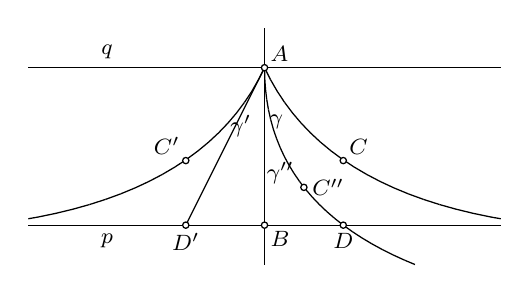
\begin{tikzpicture}
                    % \clip (0,0) rectangle (14.000000,10.000000);
                    {\footnotesize
                    
                    % Drawing line A B
                    \draw [line width=0.016cm] (4.000000,1.500000) -- (4.000000,1.960000);%
                    \draw [line width=0.016cm] (4.000000,2.040000) -- (4.000000,3.960000);%
                    \draw [line width=0.016cm] (4.000000,4.040000) -- (4.000000,4.500000);%
                    
                    % Drawing line A q
                    \draw [line width=0.016cm] (1.000000,4.000000) -- (3.960000,4.000000);%
                    \draw [line width=0.016cm] (4.040000,4.000000) -- (7.000000,4.000000);%
                    
                    % Drawing line B p
                    \draw [line width=0.016cm] (1.000000,2.000000) -- (2.960000,2.000000);%
                    \draw [line width=0.016cm] (3.040000,2.000000) -- (3.960000,2.000000);%
                    \draw [line width=0.016cm] (4.040000,2.000000) -- (4.960000,2.000000);%
                    \draw [line width=0.016cm] (5.040000,2.000000) -- (7.000000,2.000000);%
                    
                    % Drawing segment A D'
                    \draw [line width=0.016cm] (3.982111,3.964223) -- (3.017889,2.035777);%
                    
                    % Drawing Bezier curve A U X
                    \draw [line width=0.016cm] (3.923611,3.847377) -- (3.982097,3.964230);%
                    \draw [line width=0.016cm] (3.838889,3.700617) -- (3.923611,3.847377);%
                    \draw [line width=0.016cm] (3.745833,3.559722) -- (3.838889,3.700617);%
                    \draw [line width=0.016cm] (3.644444,3.424691) -- (3.745833,3.559722);%
                    \draw [line width=0.016cm] (3.534722,3.295525) -- (3.644444,3.424691);%
                    \draw [line width=0.016cm] (3.416667,3.172222) -- (3.534722,3.295525);%
                    \draw [line width=0.016cm] (3.290278,3.054784) -- (3.416667,3.172222);%
                    \draw [line width=0.016cm] (3.155556,2.943210) -- (3.290278,3.054784);%
                    \draw [line width=0.016cm] (3.027773,2.848786) -- (3.155556,2.943210);%
                    \draw [line width=0.016cm] (2.861111,2.737654) -- (2.962983,2.804842);%
                    \draw [line width=0.016cm] (2.701389,2.643673) -- (2.861111,2.737654);%
                    \draw [line width=0.016cm] (2.533333,2.555556) -- (2.701389,2.643673);%
                    \draw [line width=0.016cm] (2.356944,2.473302) -- (2.533333,2.555556);%
                    \draw [line width=0.016cm] (2.172222,2.396914) -- (2.356944,2.473302);%
                    \draw [line width=0.016cm] (1.979167,2.326389) -- (2.172222,2.396914);%
                    \draw [line width=0.016cm] (1.777778,2.261728) -- (1.979167,2.326389);%
                    \draw [line width=0.016cm] (1.568056,2.202932) -- (1.777778,2.261728);%
                    \draw [line width=0.016cm] (1.350000,2.150000) -- (1.568056,2.202932);%
                    \draw [line width=0.016cm] (1.123611,2.102932) -- (1.350000,2.150000);%
                    \draw [line width=0.016cm] (1.000000,2.081233) -- (1.123611,2.102932);%
                    
                    % Drawing Bezier curve A U' Y
                    \draw [line width=0.016cm] (4.076389,3.847377) -- (4.017903,3.964230);%
                    \draw [line width=0.016cm] (4.161111,3.700617) -- (4.076389,3.847377);%
                    \draw [line width=0.016cm] (4.254167,3.559722) -- (4.161111,3.700617);%
                    \draw [line width=0.016cm] (4.355556,3.424691) -- (4.254167,3.559722);%
                    \draw [line width=0.016cm] (4.465278,3.295525) -- (4.355556,3.424691);%
                    \draw [line width=0.016cm] (4.583333,3.172222) -- (4.465278,3.295525);%
                    \draw [line width=0.016cm] (4.709722,3.054784) -- (4.583333,3.172222);%
                    \draw [line width=0.016cm] (4.844444,2.943210) -- (4.709722,3.054784);%
                    \draw [line width=0.016cm] (4.972227,2.848786) -- (4.844444,2.943210);%
                    \draw [line width=0.016cm] (5.138889,2.737654) -- (5.037017,2.804842);%
                    \draw [line width=0.016cm] (5.298611,2.643673) -- (5.138889,2.737654);%
                    \draw [line width=0.016cm] (5.466667,2.555556) -- (5.298611,2.643673);%
                    \draw [line width=0.016cm] (5.643056,2.473302) -- (5.466667,2.555556);%
                    \draw [line width=0.016cm] (5.827778,2.396914) -- (5.643056,2.473302);%
                    \draw [line width=0.016cm] (6.020833,2.326389) -- (5.827778,2.396914);%
                    \draw [line width=0.016cm] (6.222222,2.261728) -- (6.020833,2.326389);%
                    \draw [line width=0.016cm] (6.431944,2.202932) -- (6.222222,2.261728);%
                    \draw [line width=0.016cm] (6.650000,2.150000) -- (6.431944,2.202932);%
                    \draw [line width=0.016cm] (6.876389,2.102932) -- (6.650000,2.150000);%
                    \draw [line width=0.016cm] (6.876389,2.102932) -- (7.000000,2.081233);%
                    
                    % Drawing Bezier curve A U'' Z
                    \draw [line width=0.016cm] (4.003086,3.862654) -- (4.000899,3.960010);%
                    \draw [line width=0.016cm] (4.012346,3.728395) -- (4.003086,3.862654);%
                    \draw [line width=0.016cm] (4.027778,3.597222) -- (4.012346,3.728395);%
                    \draw [line width=0.016cm] (4.049383,3.469136) -- (4.027778,3.597222);%
                    \draw [line width=0.016cm] (4.077160,3.344136) -- (4.049383,3.469136);%
                    \draw [line width=0.016cm] (4.111111,3.222222) -- (4.077160,3.344136);%
                    \draw [line width=0.016cm] (4.151235,3.103395) -- (4.111111,3.222222);%
                    \draw [line width=0.016cm] (4.197531,2.987654) -- (4.151235,3.103395);%
                    \draw [line width=0.016cm] (4.250000,2.875000) -- (4.197531,2.987654);%
                    \draw [line width=0.016cm] (4.308642,2.765432) -- (4.250000,2.875000);%
                    \draw [line width=0.016cm] (4.373457,2.658951) -- (4.308642,2.765432);%
                    \draw [line width=0.016cm] (4.444444,2.555556) -- (4.373457,2.658951);%
                    \draw [line width=0.016cm] (4.477254,2.512903) -- (4.444444,2.555556);%
                    \draw [line width=0.016cm] (4.604938,2.358025) -- (4.526255,2.449822);%
                    \draw [line width=0.016cm] (4.694444,2.263889) -- (4.604938,2.358025);%
                    \draw [line width=0.016cm] (4.790123,2.172840) -- (4.694444,2.263889);%
                    \draw [line width=0.016cm] (4.891975,2.084877) -- (4.790123,2.172840);%
                    \draw [line width=0.016cm] (4.968547,2.024713) -- (4.891975,2.084877);%
                    \draw [line width=0.016cm] (5.114198,1.918210) -- (5.032520,1.976709);%
                    \draw [line width=0.016cm] (5.234568,1.839506) -- (5.114198,1.918210);%
                    \draw [line width=0.016cm] (5.361111,1.763889) -- (5.234568,1.839506);%
                    \draw [line width=0.016cm] (5.493827,1.691358) -- (5.361111,1.763889);%
                    \draw [line width=0.016cm] (5.632716,1.621914) -- (5.493827,1.691358);%
                    \draw [line width=0.016cm] (5.777778,1.555556) -- (5.632716,1.621914);%
                    \draw [line width=0.016cm] (5.910569,1.500000) -- (5.777778,1.555556);%
                    
                    % Marking point A by circle
                    \draw [line width=0.016cm] (4.000000,4.000000) circle (0.040000);%
                    \draw (3.970000,3.970000) node [anchor=south west] { $A$ };%
                    
                    % Marking point B by circle
                    \draw [line width=0.016cm] (4.000000,2.000000) circle (0.040000);%
                    \draw (3.970000,2.030000) node [anchor=north west] { $B$ };%
                    
                    % Marking point p
                    \draw (2.000000,2.000000) node [anchor=north] { $p$ };%
                    
                    % Marking point q
                    \draw (2.000000,4.000000) node [anchor=south] { $q$ };%
                    
                    % Marking point C by circle
                    \draw [line width=0.016cm] (5.000000,2.820000) circle (0.040000);%
                    \draw (4.970000,2.790000) node [anchor=south west] { $C$ };%
                    
                    % Marking point C' by circle
                    \draw [line width=0.016cm] (3.000000,2.820000) circle (0.040000);%
                    \draw (3.030000,2.790000) node [anchor=south east] { $C'$ };%
                    
                    % Marking point D by circle
                    \draw [line width=0.016cm] (5.000000,2.000000) circle (0.040000);%
                    \draw (5.000000,2.000000) node [anchor=north] { $D$ };%
                    
                    % Marking point D' by circle
                    \draw [line width=0.016cm] (3.000000,2.000000) circle (0.040000);%
                    \draw (3.000000,2.000000) node [anchor=north] { $D'$ };%
                    
                    % Marking point C'' by circle
                    \draw [line width=0.016cm] (4.500000,2.480000) circle (0.040000);%
                    \draw (4.500000,2.480000) node [anchor=west] { $C''$ };%
                    
                    % Marking point \gamma
                    \draw (4.150000,3.500000) node [anchor=north] { $\gamma$ };%
                    
                    % Marking point \gamma'
                    \draw (3.700000,3.500000) node [anchor=north] { $\gamma'$ };%
                    
                    % Marking point \gamma''
                    \draw (4.200000,2.900000) node [anchor=north] { $\gamma''$ };%
                    }
                \end{tikzpicture}                
            \\ Če temu ni tako, recimo, da je $\gamma>\gamma'$. Potem obstaja točka $C''$ znotraj kota $\angle BAC$, da je $|\angle BAC''|=\gamma'$ in po lastnosti točke $C$ poltrak $\overrightarrow{AC''}$ seka premico $p$ v točki $D$. Naj bo točka $D'\in p$ taka, da je $B'\ast B\ast D$ in $D'B\cong BD$. Po kriteriju SKS sledi skladnost trikotnikov $\triangle D'BA\cong \triangle DBA$. Od tod pa $|\angle D'BA|=\gamma'$. To nam da protislovje $\overrightarrow{AD'}=\overrightarrow{AC'}$ s tem, da $\overrightarrow{AD'}$ seka premico $p$, $\overrightarrow{AC'}$ pa premice $p$ ne seka.
        \end{dokaz}

    \begin{definicija}
        Kota $\angle BAC$ in $\angle BAC'$ imenujemo \textbf{kota vzporednosti} v točki $A$ za premico $p$. Oznaka: $\Pi(A,p)$.
    \end{definicija}

    \begin{trditev}
        Če je premica $q$ vzporednica k premici $p$, ki vsebuje asimptotični poltrak, potem premici $p$ in $q$ nimata skupne pravokotnice.
    \end{trditev}

        \begin{dokaz}
            \\ 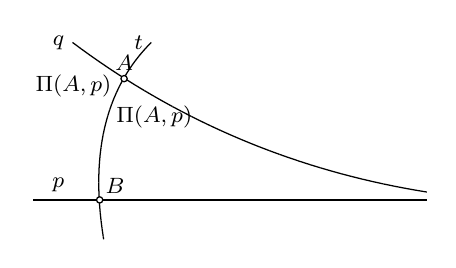
\begin{tikzpicture}
                    % \clip (0,0) rectangle (14.000000,10.000000);
                    {\footnotesize
                    
                    % Drawing line p X
                    \draw [line width=0.016cm] (1.500000,2.000000) -- (2.305000,2.000000);%
                    \draw [line width=0.016cm] (2.385000,2.000000) -- (6.500000,2.000000);%
                    
                    % Drawing Bezier curve q U Y
                    \draw [line width=0.016cm] (2.111497,3.917515) -- (2.000000,4.000000);%
                    \draw [line width=0.016cm] (2.223765,3.836728) -- (2.111497,3.917515);%
                    \draw [line width=0.016cm] (2.336806,3.757639) -- (2.223765,3.836728);%
                    \draw [line width=0.016cm] (2.450617,3.680247) -- (2.336806,3.757639);%
                    \draw [line width=0.016cm] (2.565201,3.604552) -- (2.450617,3.680247);%
                    \draw [line width=0.016cm] (2.624851,3.566288) -- (2.565201,3.604552);%
                    \draw [line width=0.016cm] (2.796682,3.458256) -- (2.691537,3.523719);%
                    \draw [line width=0.016cm] (2.913580,3.387654) -- (2.796682,3.458256);%
                    \draw [line width=0.016cm] (3.031250,3.318750) -- (2.913580,3.387654);%
                    \draw [line width=0.016cm] (3.149691,3.251543) -- (3.031250,3.318750);%
                    \draw [line width=0.016cm] (3.268904,3.186034) -- (3.149691,3.251543);%
                    \draw [line width=0.016cm] (3.388889,3.122222) -- (3.268904,3.186034);%
                    \draw [line width=0.016cm] (3.509645,3.060108) -- (3.388889,3.122222);%
                    \draw [line width=0.016cm] (3.631173,2.999691) -- (3.509645,3.060108);%
                    \draw [line width=0.016cm] (3.753472,2.940972) -- (3.631173,2.999691);%
                    \draw [line width=0.016cm] (3.876543,2.883951) -- (3.753472,2.940972);%
                    \draw [line width=0.016cm] (4.000386,2.828627) -- (3.876543,2.883951);%
                    \draw [line width=0.016cm] (4.125000,2.775000) -- (4.000386,2.828627);%
                    \draw [line width=0.016cm] (4.250386,2.723071) -- (4.125000,2.775000);%
                    \draw [line width=0.016cm] (4.376543,2.672840) -- (4.250386,2.723071);%
                    \draw [line width=0.016cm] (4.503472,2.624306) -- (4.376543,2.672840);%
                    \draw [line width=0.016cm] (4.631173,2.577469) -- (4.503472,2.624306);%
                    \draw [line width=0.016cm] (4.759645,2.532330) -- (4.631173,2.577469);%
                    \draw [line width=0.016cm] (4.888889,2.488889) -- (4.759645,2.532330);%
                    \draw [line width=0.016cm] (5.018904,2.447145) -- (4.888889,2.488889);%
                    \draw [line width=0.016cm] (5.149691,2.407099) -- (5.018904,2.447145);%
                    \draw [line width=0.016cm] (5.281250,2.368750) -- (5.149691,2.407099);%
                    \draw [line width=0.016cm] (5.413580,2.332099) -- (5.281250,2.368750);%
                    \draw [line width=0.016cm] (5.546682,2.297145) -- (5.413580,2.332099);%
                    \draw [line width=0.016cm] (5.680556,2.263889) -- (5.546682,2.297145);%
                    \draw [line width=0.016cm] (5.815201,2.232330) -- (5.680556,2.263889);%
                    \draw [line width=0.016cm] (5.950617,2.202469) -- (5.815201,2.232330);%
                    \draw [line width=0.016cm] (6.086806,2.174306) -- (5.950617,2.202469);%
                    \draw [line width=0.016cm] (6.223765,2.147840) -- (6.086806,2.174306);%
                    \draw [line width=0.016cm] (6.361497,2.123071) -- (6.223765,2.147840);%
                    \draw [line width=0.016cm] (6.500000,2.100000) -- (6.361497,2.123071);%
                    
                    % Drawing Bezier curve t V Z
                    \draw [line width=0.016cm] (2.945602,3.943673) -- (3.000000,4.000000);%
                    \draw [line width=0.016cm] (2.893519,3.885802) -- (2.945602,3.943673);%
                    \draw [line width=0.016cm] (2.843750,3.826389) -- (2.893519,3.885802);%
                    \draw [line width=0.016cm] (2.796296,3.765432) -- (2.843750,3.826389);%
                    \draw [line width=0.016cm] (2.751157,3.702932) -- (2.796296,3.765432);%
                    \draw [line width=0.016cm] (2.708333,3.638889) -- (2.751157,3.702932);%
                    \draw [line width=0.016cm] (2.670126,3.577030) -- (2.708333,3.638889);%
                    \draw [line width=0.016cm] (2.629630,3.506173) -- (2.630769,3.508175);%
                    \draw [line width=0.016cm] (2.593750,3.437500) -- (2.629630,3.506173);%
                    \draw [line width=0.016cm] (2.560185,3.367284) -- (2.593750,3.437500);%
                    \draw [line width=0.016cm] (2.528935,3.295525) -- (2.560185,3.367284);%
                    \draw [line width=0.016cm] (2.500000,3.222222) -- (2.528935,3.295525);%
                    \draw [line width=0.016cm] (2.473380,3.147377) -- (2.500000,3.222222);%
                    \draw [line width=0.016cm] (2.449074,3.070988) -- (2.473380,3.147377);%
                    \draw [line width=0.016cm] (2.427083,2.993056) -- (2.449074,3.070988);%
                    \draw [line width=0.016cm] (2.407407,2.913580) -- (2.427083,2.993056);%
                    \draw [line width=0.016cm] (2.390046,2.832562) -- (2.407407,2.913580);%
                    \draw [line width=0.016cm] (2.375000,2.750000) -- (2.390046,2.832562);%
                    \draw [line width=0.016cm] (2.362269,2.665895) -- (2.375000,2.750000);%
                    \draw [line width=0.016cm] (2.351852,2.580247) -- (2.362269,2.665895);%
                    \draw [line width=0.016cm] (2.343750,2.493056) -- (2.351852,2.580247);%
                    \draw [line width=0.016cm] (2.337963,2.404321) -- (2.343750,2.493056);%
                    \draw [line width=0.016cm] (2.334491,2.314043) -- (2.337963,2.404321);%
                    \draw [line width=0.016cm] (2.333333,2.222222) -- (2.334491,2.314043);%
                    \draw [line width=0.016cm] (2.334491,2.128858) -- (2.333333,2.222222);%
                    \draw [line width=0.016cm] (2.337766,2.039340) -- (2.334491,2.128858);%
                    \draw [line width=0.016cm] (2.343750,1.937500) -- (2.342395,1.960085);%
                    \draw [line width=0.016cm] (2.351852,1.839506) -- (2.343750,1.937500);%
                    \draw [line width=0.016cm] (2.362269,1.739969) -- (2.351852,1.839506);%
                    \draw [line width=0.016cm] (2.375000,1.638889) -- (2.362269,1.739969);%
                    \draw [line width=0.016cm] (2.390046,1.536265) -- (2.375000,1.638889);%
                    \draw [line width=0.016cm] (2.396091,1.500000) -- (2.390046,1.536265);%
                    
                    % Marking point t
                    \draw (3.000000,4.000000) node [anchor=east] { $t$ };%
                    
                    % Marking point q
                    \draw (2.000000,4.000000) node [anchor=east] { $q$ };%
                    
                    % Marking point p
                    \draw (2.000000,2.000000) node [anchor=south east] { $p$ };%
                    
                    % Marking point A by circle
                    \draw [line width=0.016cm] (2.655000,3.540000) circle (0.040000);%
                    \draw (2.655000,3.540000) node [anchor=south] { $A$ };%
                    
                    % Marking point B by circle
                    \draw [line width=0.016cm] (2.345000,2.000000) circle (0.040000);%
                    \draw (2.315000,1.970000) node [anchor=south west] { $B$ };%
                    
                    % Marking point \Pi(A,p)
                    \draw (2.450000,3.300000) node [anchor=north west] { $\Pi(A,p)$ };%
                    
                    % Marking point \Pi(A,p)
                    \draw (2.600000,3.700000) node [anchor=north east] { $\Pi(A,p)$ };%
                    }
                \end{tikzpicture}                
            \\ Če bi obstajala skupna pravokotnica $t$, potem je $\Pi(A,p)=\frac{\pi}{2}$ in zato je premica $q$ edina vzporednika k premici $p$ skozi točko $A$. To nas privede v protislovje.
        \end{dokaz}

    \begin{opomba}
        Zgornje pokaže, da so asimptotične in divergentne vzporednice res različne. Res gre razdalja med asimptotičnima poltrakoma proti $0$. Zgornje sta edina tipa vzporednic.
    \end{opomba}

    \begin{definicija}[ekvivalenca poltrakov]
        Poltraka $\overrightarrow{AB}$ in $\overrightarrow{CD}$ sta ekvivalenta, če velja eden od naslednjih pogojev: $\overrightarrow{AB} \subseteq  \overrightarrow{CD}$ ali $\overrightarrow{AB} \supseteq  \overrightarrow{CD}$ ali $\overrightarrow{AB}$ in $\overrightarrow{CD}$ sta asimptotična. Ekviivalncčni razred poltrakov imenujemo \textbf{idealna točka} (ali \textbf{konec}).
    \end{definicija}

    \begin{opomba}
        \begin{enumerate}
            \item Šteli bomo, da idealna točka leži na vseh poltrakih, ki jo določajo.
            \item Idealne točke bomo označevali z velikimi grškimi črkami ($\Omega$, $\Sigma$, ...). Tak poltrak $\overrightarrow{AB}$, ki določa idealno točko $\Omega$ bomo pisali tudi $\overrightarrow{A\Omega}$/$A\Omega$.
            \item Vsaka premica vsebuje dve idealni točki, na vsakem koncu eno. Posebej to pomeni, da množica idealnih točk ni premica.
        \end{enumerate}
    \end{opomba}

    \begin{definicija}
        Naj bosta $A$ in $B$ različni točki in $\Omega$ idealna točka. Potem je \textbf{enojno asimptotičen} trikotnik $\triangle AB\Omega$ omejen z daljico $AB$ in poltrakoma $\overrightarrow{A\Omega}$ in $\overrightarrow{B\Omega}$. Podobno definiramo dvojno in trojno asimptotične trikotnike.
    \end{definicija}

        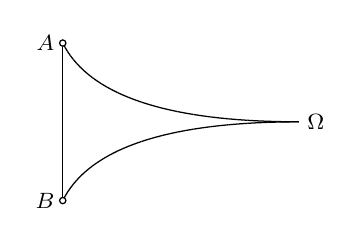
\begin{tikzpicture}
            % \clip (0,0) rectangle (14.000000,10.000000);
            {\footnotesize
            
            % Drawing segment A B
            \draw [line width=0.016cm] (2.000000,3.960000) -- (2.000000,2.040000);%
            
            % Drawing Bezier curve A X \Omega
            \draw [line width=0.016cm] (2.029321,3.945216) -- (2.018875,3.964733);%
            \draw [line width=0.016cm] (2.061728,3.891975) -- (2.029321,3.945216);%
            \draw [line width=0.016cm] (2.097222,3.840278) -- (2.061728,3.891975);%
            \draw [line width=0.016cm] (2.135802,3.790123) -- (2.097222,3.840278);%
            \draw [line width=0.016cm] (2.177469,3.741512) -- (2.135802,3.790123);%
            \draw [line width=0.016cm] (2.222222,3.694444) -- (2.177469,3.741512);%
            \draw [line width=0.016cm] (2.270062,3.648920) -- (2.222222,3.694444);%
            \draw [line width=0.016cm] (2.320988,3.604938) -- (2.270062,3.648920);%
            \draw [line width=0.016cm] (2.375000,3.562500) -- (2.320988,3.604938);%
            \draw [line width=0.016cm] (2.432099,3.521605) -- (2.375000,3.562500);%
            \draw [line width=0.016cm] (2.492284,3.482253) -- (2.432099,3.521605);%
            \draw [line width=0.016cm] (2.555556,3.444444) -- (2.492284,3.482253);%
            \draw [line width=0.016cm] (2.621914,3.408179) -- (2.555556,3.444444);%
            \draw [line width=0.016cm] (2.691358,3.373457) -- (2.621914,3.408179);%
            \draw [line width=0.016cm] (2.763889,3.340278) -- (2.691358,3.373457);%
            \draw [line width=0.016cm] (2.839506,3.308642) -- (2.763889,3.340278);%
            \draw [line width=0.016cm] (2.918210,3.278549) -- (2.839506,3.308642);%
            \draw [line width=0.016cm] (3.000000,3.250000) -- (2.918210,3.278549);%
            \draw [line width=0.016cm] (3.084877,3.222994) -- (3.000000,3.250000);%
            \draw [line width=0.016cm] (3.172840,3.197531) -- (3.084877,3.222994);%
            \draw [line width=0.016cm] (3.263889,3.173611) -- (3.172840,3.197531);%
            \draw [line width=0.016cm] (3.358025,3.151235) -- (3.263889,3.173611);%
            \draw [line width=0.016cm] (3.455247,3.130401) -- (3.358025,3.151235);%
            \draw [line width=0.016cm] (3.555556,3.111111) -- (3.455247,3.130401);%
            \draw [line width=0.016cm] (3.658951,3.093364) -- (3.555556,3.111111);%
            \draw [line width=0.016cm] (3.765432,3.077160) -- (3.658951,3.093364);%
            \draw [line width=0.016cm] (3.875000,3.062500) -- (3.765432,3.077160);%
            \draw [line width=0.016cm] (3.987654,3.049383) -- (3.875000,3.062500);%
            \draw [line width=0.016cm] (4.103395,3.037809) -- (3.987654,3.049383);%
            \draw [line width=0.016cm] (4.222222,3.027778) -- (4.103395,3.037809);%
            \draw [line width=0.016cm] (4.344136,3.019290) -- (4.222222,3.027778);%
            \draw [line width=0.016cm] (4.469136,3.012346) -- (4.344136,3.019290);%
            \draw [line width=0.016cm] (4.597222,3.006944) -- (4.469136,3.012346);%
            \draw [line width=0.016cm] (4.728395,3.003086) -- (4.597222,3.006944);%
            \draw [line width=0.016cm] (4.862654,3.000772) -- (4.728395,3.003086);%
            \draw [line width=0.016cm] (5.000000,3.000000) -- (4.862654,3.000772);%
            
            % Drawing Bezier curve B X \Omega
            \draw [line width=0.016cm] (2.029321,2.054784) -- (2.018875,2.035267);%
            \draw [line width=0.016cm] (2.061728,2.108025) -- (2.029321,2.054784);%
            \draw [line width=0.016cm] (2.097222,2.159722) -- (2.061728,2.108025);%
            \draw [line width=0.016cm] (2.135802,2.209877) -- (2.097222,2.159722);%
            \draw [line width=0.016cm] (2.177469,2.258488) -- (2.135802,2.209877);%
            \draw [line width=0.016cm] (2.222222,2.305556) -- (2.177469,2.258488);%
            \draw [line width=0.016cm] (2.270062,2.351080) -- (2.222222,2.305556);%
            \draw [line width=0.016cm] (2.320988,2.395062) -- (2.270062,2.351080);%
            \draw [line width=0.016cm] (2.375000,2.437500) -- (2.320988,2.395062);%
            \draw [line width=0.016cm] (2.432099,2.478395) -- (2.375000,2.437500);%
            \draw [line width=0.016cm] (2.492284,2.517747) -- (2.432099,2.478395);%
            \draw [line width=0.016cm] (2.555556,2.555556) -- (2.492284,2.517747);%
            \draw [line width=0.016cm] (2.621914,2.591821) -- (2.555556,2.555556);%
            \draw [line width=0.016cm] (2.691358,2.626543) -- (2.621914,2.591821);%
            \draw [line width=0.016cm] (2.763889,2.659722) -- (2.691358,2.626543);%
            \draw [line width=0.016cm] (2.839506,2.691358) -- (2.763889,2.659722);%
            \draw [line width=0.016cm] (2.918210,2.721451) -- (2.839506,2.691358);%
            \draw [line width=0.016cm] (3.000000,2.750000) -- (2.918210,2.721451);%
            \draw [line width=0.016cm] (3.084877,2.777006) -- (3.000000,2.750000);%
            \draw [line width=0.016cm] (3.172840,2.802469) -- (3.084877,2.777006);%
            \draw [line width=0.016cm] (3.263889,2.826389) -- (3.172840,2.802469);%
            \draw [line width=0.016cm] (3.358025,2.848765) -- (3.263889,2.826389);%
            \draw [line width=0.016cm] (3.455247,2.869599) -- (3.358025,2.848765);%
            \draw [line width=0.016cm] (3.555556,2.888889) -- (3.455247,2.869599);%
            \draw [line width=0.016cm] (3.658951,2.906636) -- (3.555556,2.888889);%
            \draw [line width=0.016cm] (3.765432,2.922840) -- (3.658951,2.906636);%
            \draw [line width=0.016cm] (3.875000,2.937500) -- (3.765432,2.922840);%
            \draw [line width=0.016cm] (3.987654,2.950617) -- (3.875000,2.937500);%
            \draw [line width=0.016cm] (4.103395,2.962191) -- (3.987654,2.950617);%
            \draw [line width=0.016cm] (4.222222,2.972222) -- (4.103395,2.962191);%
            \draw [line width=0.016cm] (4.344136,2.980710) -- (4.222222,2.972222);%
            \draw [line width=0.016cm] (4.469136,2.987654) -- (4.344136,2.980710);%
            \draw [line width=0.016cm] (4.597222,2.993056) -- (4.469136,2.987654);%
            \draw [line width=0.016cm] (4.728395,2.996914) -- (4.597222,2.993056);%
            \draw [line width=0.016cm] (4.862654,2.999228) -- (4.728395,2.996914);%
            \draw [line width=0.016cm] (5.000000,3.000000) -- (4.862654,2.999228);%
            
            % Marking point A by circle
            \draw [line width=0.016cm] (2.000000,4.000000) circle (0.040000);%
            \draw (2.000000,4.000000) node [anchor=east] { $A$ };%
            
            % Marking point B by circle
            \draw [line width=0.016cm] (2.000000,2.000000) circle (0.040000);%
            \draw (2.000000,2.000000) node [anchor=east] { $B$ };%
            
            % Marking point \Omega
            \draw (5.000000,3.000000) node [anchor=west] { $\Omega$ };%
            }
        \end{tikzpicture}
        
    \begin{trditev}[zunanji kot v asimptotičnem trikotniku]
        Naj bo $\triangle AB\Omega$ enojno asimptotičen trikotnik. Potem je zunanji kot pri $A$ večji od notranjega kota pri $B$ in zunanji kot pri $B$ večji od notranjega kota pri $A$.
    \end{trditev}

        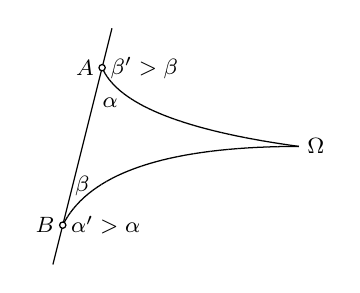
\begin{tikzpicture}
            % \clip (0,0) rectangle (14.000000,10.000000);
            {\footnotesize
            
            % Drawing line A B
            \draw [line width=0.016cm] (1.875000,1.500000) -- (1.990299,1.961194);%
            \draw [line width=0.016cm] (2.009701,2.038806) -- (2.490299,3.961194);%
            \draw [line width=0.016cm] (2.509701,4.038806) -- (2.625000,4.500000);%
            
            % Drawing Bezier curve A Y \Omega
            \draw [line width=0.016cm] (2.518133,3.961420) -- (2.517014,3.963799);%
            \draw [line width=0.016cm] (2.539198,3.923457) -- (2.518133,3.961420);%
            \draw [line width=0.016cm] (2.563194,3.886111) -- (2.539198,3.923457);%
            \draw [line width=0.016cm] (2.590123,3.849383) -- (2.563194,3.886111);%
            \draw [line width=0.016cm] (2.619985,3.813272) -- (2.590123,3.849383);%
            \draw [line width=0.016cm] (2.652778,3.777778) -- (2.619985,3.813272);%
            \draw [line width=0.016cm] (2.688503,3.742901) -- (2.652778,3.777778);%
            \draw [line width=0.016cm] (2.727160,3.708642) -- (2.688503,3.742901);%
            \draw [line width=0.016cm] (2.768750,3.675000) -- (2.727160,3.708642);%
            \draw [line width=0.016cm] (2.813272,3.641975) -- (2.768750,3.675000);%
            \draw [line width=0.016cm] (2.860725,3.609568) -- (2.813272,3.641975);%
            \draw [line width=0.016cm] (2.911111,3.577778) -- (2.860725,3.609568);%
            \draw [line width=0.016cm] (2.964429,3.546605) -- (2.911111,3.577778);%
            \draw [line width=0.016cm] (3.020679,3.516049) -- (2.964429,3.546605);%
            \draw [line width=0.016cm] (3.079861,3.486111) -- (3.020679,3.516049);%
            \draw [line width=0.016cm] (3.141975,3.456790) -- (3.079861,3.486111);%
            \draw [line width=0.016cm] (3.207022,3.428086) -- (3.141975,3.456790);%
            \draw [line width=0.016cm] (3.275000,3.400000) -- (3.207022,3.428086);%
            \draw [line width=0.016cm] (3.345910,3.372531) -- (3.275000,3.400000);%
            \draw [line width=0.016cm] (3.419753,3.345679) -- (3.345910,3.372531);%
            \draw [line width=0.016cm] (3.496528,3.319444) -- (3.419753,3.345679);%
            \draw [line width=0.016cm] (3.576235,3.293827) -- (3.496528,3.319444);%
            \draw [line width=0.016cm] (3.658873,3.268827) -- (3.576235,3.293827);%
            \draw [line width=0.016cm] (3.744444,3.244444) -- (3.658873,3.268827);%
            \draw [line width=0.016cm] (3.832948,3.220679) -- (3.744444,3.244444);%
            \draw [line width=0.016cm] (3.924383,3.197531) -- (3.832948,3.220679);%
            \draw [line width=0.016cm] (4.018750,3.175000) -- (3.924383,3.197531);%
            \draw [line width=0.016cm] (4.116049,3.153086) -- (4.018750,3.175000);%
            \draw [line width=0.016cm] (4.216281,3.131790) -- (4.116049,3.153086);%
            \draw [line width=0.016cm] (4.319444,3.111111) -- (4.216281,3.131790);%
            \draw [line width=0.016cm] (4.425540,3.091049) -- (4.319444,3.111111);%
            \draw [line width=0.016cm] (4.534568,3.071605) -- (4.425540,3.091049);%
            \draw [line width=0.016cm] (4.646528,3.052778) -- (4.534568,3.071605);%
            \draw [line width=0.016cm] (4.761420,3.034568) -- (4.646528,3.052778);%
            \draw [line width=0.016cm] (4.879244,3.016975) -- (4.761420,3.034568);%
            \draw [line width=0.016cm] (5.000000,3.000000) -- (4.879244,3.016975);%
            
            % Drawing Bezier curve B X \Omega
            \draw [line width=0.016cm] (2.029321,2.054784) -- (2.018875,2.035267);%
            \draw [line width=0.016cm] (2.061728,2.108025) -- (2.029321,2.054784);%
            \draw [line width=0.016cm] (2.097222,2.159722) -- (2.061728,2.108025);%
            \draw [line width=0.016cm] (2.135802,2.209877) -- (2.097222,2.159722);%
            \draw [line width=0.016cm] (2.177469,2.258488) -- (2.135802,2.209877);%
            \draw [line width=0.016cm] (2.222222,2.305556) -- (2.177469,2.258488);%
            \draw [line width=0.016cm] (2.270062,2.351080) -- (2.222222,2.305556);%
            \draw [line width=0.016cm] (2.320988,2.395062) -- (2.270062,2.351080);%
            \draw [line width=0.016cm] (2.375000,2.437500) -- (2.320988,2.395062);%
            \draw [line width=0.016cm] (2.432099,2.478395) -- (2.375000,2.437500);%
            \draw [line width=0.016cm] (2.492284,2.517747) -- (2.432099,2.478395);%
            \draw [line width=0.016cm] (2.555556,2.555556) -- (2.492284,2.517747);%
            \draw [line width=0.016cm] (2.621914,2.591821) -- (2.555556,2.555556);%
            \draw [line width=0.016cm] (2.691358,2.626543) -- (2.621914,2.591821);%
            \draw [line width=0.016cm] (2.763889,2.659722) -- (2.691358,2.626543);%
            \draw [line width=0.016cm] (2.839506,2.691358) -- (2.763889,2.659722);%
            \draw [line width=0.016cm] (2.918210,2.721451) -- (2.839506,2.691358);%
            \draw [line width=0.016cm] (3.000000,2.750000) -- (2.918210,2.721451);%
            \draw [line width=0.016cm] (3.084877,2.777006) -- (3.000000,2.750000);%
            \draw [line width=0.016cm] (3.172840,2.802469) -- (3.084877,2.777006);%
            \draw [line width=0.016cm] (3.263889,2.826389) -- (3.172840,2.802469);%
            \draw [line width=0.016cm] (3.358025,2.848765) -- (3.263889,2.826389);%
            \draw [line width=0.016cm] (3.455247,2.869599) -- (3.358025,2.848765);%
            \draw [line width=0.016cm] (3.555556,2.888889) -- (3.455247,2.869599);%
            \draw [line width=0.016cm] (3.658951,2.906636) -- (3.555556,2.888889);%
            \draw [line width=0.016cm] (3.765432,2.922840) -- (3.658951,2.906636);%
            \draw [line width=0.016cm] (3.875000,2.937500) -- (3.765432,2.922840);%
            \draw [line width=0.016cm] (3.987654,2.950617) -- (3.875000,2.937500);%
            \draw [line width=0.016cm] (4.103395,2.962191) -- (3.987654,2.950617);%
            \draw [line width=0.016cm] (4.222222,2.972222) -- (4.103395,2.962191);%
            \draw [line width=0.016cm] (4.344136,2.980710) -- (4.222222,2.972222);%
            \draw [line width=0.016cm] (4.469136,2.987654) -- (4.344136,2.980710);%
            \draw [line width=0.016cm] (4.597222,2.993056) -- (4.469136,2.987654);%
            \draw [line width=0.016cm] (4.728395,2.996914) -- (4.597222,2.993056);%
            \draw [line width=0.016cm] (4.862654,2.999228) -- (4.728395,2.996914);%
            \draw [line width=0.016cm] (5.000000,3.000000) -- (4.862654,2.999228);%
            
            % Marking point A by circle
            \draw [line width=0.016cm] (2.500000,4.000000) circle (0.040000);%
            \draw (2.500000,4.000000) node [anchor=east] { $A$ };%
            
            % Marking point B by circle
            \draw [line width=0.016cm] (2.000000,2.000000) circle (0.040000);%
            \draw (2.000000,2.000000) node [anchor=east] { $B$ };%
            
            % Marking point \Omega
            \draw (5.000000,3.000000) node [anchor=west] { $\Omega$ };%
            
            % Marking point \beta
            \draw (2.050000,2.500000) node [anchor=west] { $\beta$ };%
            
            % Marking point \alpha
            \draw (2.400000,3.550000) node [anchor=west] { $\alpha$ };%
            
            % Marking point \beta'>\beta
            \draw (2.500000,4.000000) node [anchor=west] { $\beta'>\beta$ };%
            
            % Marking point \alpha'>\alpha
            \draw (2.000000,2.000000) node [anchor=west] { $\alpha'>\alpha$ };%
            }
        \end{tikzpicture}

        \begin{dokaz}
            \\ Naj bo točka $C$ taka, da premica $\overleftrightarrow{BC}$ s premico $\overleftrightarrow{AB}$ oklepa kot $\alpha$. Vemo, da je premica $\overleftrightarrow{BC}$ vzporedna premici, ki nosi poltrak $\overrightarrow{A\Omega}$. Še več, ti dve premici sta divergentno vzporedni.
            \\ 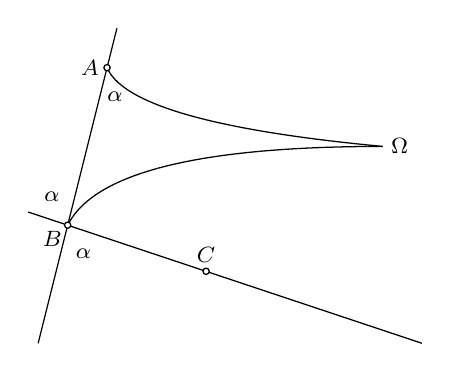
\begin{tikzpicture}
                    % \clip (0,0) rectangle (14.000000,10.000000);
                    {\footnotesize
                    
                    % Drawing line A B
                    \draw [line width=0.016cm] (1.625000,1.500000) -- (1.990299,2.961194);%
                    \draw [line width=0.016cm] (2.009701,3.038806) -- (2.490299,4.961194);%
                    \draw [line width=0.016cm] (2.509701,5.038806) -- (2.625000,5.500000);%
                    
                    % Drawing Bezier curve A Y \Omega
                    \draw [line width=0.016cm] (2.518904,4.961420) -- (2.517601,4.964080);%
                    \draw [line width=0.016cm] (2.542284,4.923457) -- (2.518904,4.961420);%
                    \draw [line width=0.016cm] (2.570139,4.886111) -- (2.542284,4.923457);%
                    \draw [line width=0.016cm] (2.602469,4.849383) -- (2.570139,4.886111);%
                    \draw [line width=0.016cm] (2.639275,4.813272) -- (2.602469,4.849383);%
                    \draw [line width=0.016cm] (2.680556,4.777778) -- (2.639275,4.813272);%
                    \draw [line width=0.016cm] (2.726312,4.742901) -- (2.680556,4.777778);%
                    \draw [line width=0.016cm] (2.776543,4.708642) -- (2.726312,4.742901);%
                    \draw [line width=0.016cm] (2.831250,4.675000) -- (2.776543,4.708642);%
                    \draw [line width=0.016cm] (2.890432,4.641975) -- (2.831250,4.675000);%
                    \draw [line width=0.016cm] (2.954090,4.609568) -- (2.890432,4.641975);%
                    \draw [line width=0.016cm] (3.022222,4.577778) -- (2.954090,4.609568);%
                    \draw [line width=0.016cm] (3.094830,4.546605) -- (3.022222,4.577778);%
                    \draw [line width=0.016cm] (3.171914,4.516049) -- (3.094830,4.546605);%
                    \draw [line width=0.016cm] (3.253472,4.486111) -- (3.171914,4.516049);%
                    \draw [line width=0.016cm] (3.339506,4.456790) -- (3.253472,4.486111);%
                    \draw [line width=0.016cm] (3.430015,4.428086) -- (3.339506,4.456790);%
                    \draw [line width=0.016cm] (3.525000,4.400000) -- (3.430015,4.428086);%
                    \draw [line width=0.016cm] (3.624460,4.372531) -- (3.525000,4.400000);%
                    \draw [line width=0.016cm] (3.728395,4.345679) -- (3.624460,4.372531);%
                    \draw [line width=0.016cm] (3.836806,4.319444) -- (3.728395,4.345679);%
                    \draw [line width=0.016cm] (3.949691,4.293827) -- (3.836806,4.319444);%
                    \draw [line width=0.016cm] (4.067052,4.268827) -- (3.949691,4.293827);%
                    \draw [line width=0.016cm] (4.188889,4.244444) -- (4.067052,4.268827);%
                    \draw [line width=0.016cm] (4.315201,4.220679) -- (4.188889,4.244444);%
                    \draw [line width=0.016cm] (4.445988,4.197531) -- (4.315201,4.220679);%
                    \draw [line width=0.016cm] (4.581250,4.175000) -- (4.445988,4.197531);%
                    \draw [line width=0.016cm] (4.720988,4.153086) -- (4.581250,4.175000);%
                    \draw [line width=0.016cm] (4.865201,4.131790) -- (4.720988,4.153086);%
                    \draw [line width=0.016cm] (5.013889,4.111111) -- (4.865201,4.131790);%
                    \draw [line width=0.016cm] (5.167052,4.091049) -- (5.013889,4.111111);%
                    \draw [line width=0.016cm] (5.324691,4.071605) -- (5.167052,4.091049);%
                    \draw [line width=0.016cm] (5.486806,4.052778) -- (5.324691,4.071605);%
                    \draw [line width=0.016cm] (5.653395,4.034568) -- (5.486806,4.052778);%
                    \draw [line width=0.016cm] (5.824460,4.016975) -- (5.653395,4.034568);%
                    \draw [line width=0.016cm] (6.000000,4.000000) -- (5.824460,4.016975);%
                    
                    % Drawing Bezier curve B X \Omega
                    \draw [line width=0.016cm] (2.030093,3.054784) -- (2.019258,3.035059);%
                    \draw [line width=0.016cm] (2.064815,3.108025) -- (2.030093,3.054784);%
                    \draw [line width=0.016cm] (2.104167,3.159722) -- (2.064815,3.108025);%
                    \draw [line width=0.016cm] (2.148148,3.209877) -- (2.104167,3.159722);%
                    \draw [line width=0.016cm] (2.196759,3.258488) -- (2.148148,3.209877);%
                    \draw [line width=0.016cm] (2.250000,3.305556) -- (2.196759,3.258488);%
                    \draw [line width=0.016cm] (2.307870,3.351080) -- (2.250000,3.305556);%
                    \draw [line width=0.016cm] (2.370370,3.395062) -- (2.307870,3.351080);%
                    \draw [line width=0.016cm] (2.437500,3.437500) -- (2.370370,3.395062);%
                    \draw [line width=0.016cm] (2.509259,3.478395) -- (2.437500,3.437500);%
                    \draw [line width=0.016cm] (2.585648,3.517747) -- (2.509259,3.478395);%
                    \draw [line width=0.016cm] (2.666667,3.555556) -- (2.585648,3.517747);%
                    \draw [line width=0.016cm] (2.752315,3.591821) -- (2.666667,3.555556);%
                    \draw [line width=0.016cm] (2.842593,3.626543) -- (2.752315,3.591821);%
                    \draw [line width=0.016cm] (2.937500,3.659722) -- (2.842593,3.626543);%
                    \draw [line width=0.016cm] (3.037037,3.691358) -- (2.937500,3.659722);%
                    \draw [line width=0.016cm] (3.141204,3.721451) -- (3.037037,3.691358);%
                    \draw [line width=0.016cm] (3.250000,3.750000) -- (3.141204,3.721451);%
                    \draw [line width=0.016cm] (3.363426,3.777006) -- (3.250000,3.750000);%
                    \draw [line width=0.016cm] (3.481481,3.802469) -- (3.363426,3.777006);%
                    \draw [line width=0.016cm] (3.604167,3.826389) -- (3.481481,3.802469);%
                    \draw [line width=0.016cm] (3.731481,3.848765) -- (3.604167,3.826389);%
                    \draw [line width=0.016cm] (3.863426,3.869599) -- (3.731481,3.848765);%
                    \draw [line width=0.016cm] (4.000000,3.888889) -- (3.863426,3.869599);%
                    \draw [line width=0.016cm] (4.141204,3.906636) -- (4.000000,3.888889);%
                    \draw [line width=0.016cm] (4.287037,3.922840) -- (4.141204,3.906636);%
                    \draw [line width=0.016cm] (4.437500,3.937500) -- (4.287037,3.922840);%
                    \draw [line width=0.016cm] (4.592593,3.950617) -- (4.437500,3.937500);%
                    \draw [line width=0.016cm] (4.752315,3.962191) -- (4.592593,3.950617);%
                    \draw [line width=0.016cm] (4.916667,3.972222) -- (4.752315,3.962191);%
                    \draw [line width=0.016cm] (5.085648,3.980710) -- (4.916667,3.972222);%
                    \draw [line width=0.016cm] (5.259259,3.987654) -- (5.085648,3.980710);%
                    \draw [line width=0.016cm] (5.437500,3.993056) -- (5.259259,3.987654);%
                    \draw [line width=0.016cm] (5.620370,3.996914) -- (5.437500,3.993056);%
                    \draw [line width=0.016cm] (5.807870,3.999228) -- (5.620370,3.996914);%
                    \draw [line width=0.016cm] (6.000000,4.000000) -- (5.807870,3.999228);%
                    
                    % Drawing line B Z
                    \draw [line width=0.016cm] (6.500000,1.500000) -- (3.795947,2.401351);%
                    \draw [line width=0.016cm] (3.720053,2.426649) -- (2.037947,2.987351);%
                    \draw [line width=0.016cm] (1.962053,3.012649) -- (1.500000,3.166667);%
                    
                    % Marking point A by circle
                    \draw [line width=0.016cm] (2.500000,5.000000) circle (0.040000);%
                    \draw (2.500000,5.000000) node [anchor=east] { $A$ };%
                    
                    % Marking point B by circle
                    \draw [line width=0.016cm] (2.000000,3.000000) circle (0.040000);%
                    \draw (2.030000,3.030000) node [anchor=north east] { $B$ };%
                    
                    % Marking point \Omega
                    \draw (6.000000,4.000000) node [anchor=west] { $\Omega$ };%
                    
                    % Marking point C by circle
                    \draw [line width=0.016cm] (3.758000,2.414000) circle (0.040000);%
                    \draw (3.758000,2.414000) node [anchor=south] { $C$ };%
                    
                    % Marking point \alpha
                    \draw (2.600000,4.800000) node [anchor=north] { $\alpha$ };%
                    
                    % Marking point \alpha
                    \draw (2.200000,2.800000) node [anchor=north] { $\alpha$ };%
                    
                    % Marking point \alpha
                    \draw (1.800000,3.200000) node [anchor=south] { $\alpha$ };%
                    }
                \end{tikzpicture}                
            \\ Naj bo točka $S$ razpolovišče $AB$ in točka $A'$ nožišče pravokotnice iz $S$ na $\overrightarrow{A\Omega}$, točka $B'$ pa nožišče pravokotnice iz $S$ na $\overrightarrow{BC}$. Po kriteriju SKK sledi skladnosti trikotnikov $\triangle SAA'\cong\triangle SBB'$, od tod pa skladnost kotov $\angle BSB'\cong\angle ASA'$. Torej velja naslednja kolinearnost točk: $A'\ast S\ast B'$.
            \\ 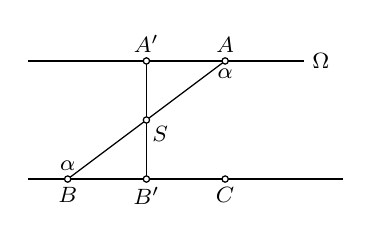
\begin{tikzpicture}
                    % \clip (0,0) rectangle (14.000000,10.000000);
                    {\footnotesize
                    
                    % Drawing segment V \Omega
                    \draw [line width=0.016cm] (1.500000,3.500000) -- (2.960000,3.500000);%
                    \draw [line width=0.016cm] (3.040000,3.500000) -- (3.960000,3.500000);%
                    \draw [line width=0.016cm] (4.040000,3.500000) -- (5.000000,3.500000);%
                    
                    % Drawing segment B' A'
                    \draw [line width=0.016cm] (3.000000,2.040000) -- (3.000000,2.710000);%
                    \draw [line width=0.016cm] (3.000000,2.790000) -- (3.000000,3.460000);%
                    
                    % Drawing segment B A
                    \draw [line width=0.016cm] (2.032000,2.024000) -- (2.968000,2.726000);%
                    \draw [line width=0.016cm] (3.032000,2.774000) -- (3.968000,3.476000);%
                    
                    % Drawing line b
                    \draw [line width=0.016cm] (1.500000,2.000000) -- (1.960000,2.000000);%
                    \draw [line width=0.016cm] (2.040000,2.000000) -- (2.960000,2.000000);%
                    \draw [line width=0.016cm] (3.040000,2.000000) -- (3.960000,2.000000);%
                    \draw [line width=0.016cm] (4.040000,2.000000) -- (5.500000,2.000000);%
                    
                    % Marking point A by circle
                    \draw [line width=0.016cm] (4.000000,3.500000) circle (0.040000);%
                    \draw (4.000000,3.500000) node [anchor=south] { $A$ };%
                    
                    % Marking point A' by circle
                    \draw [line width=0.016cm] (3.000000,3.500000) circle (0.040000);%
                    \draw (3.000000,3.500000) node [anchor=south] { $A'$ };%
                    
                    % Marking point B by circle
                    \draw [line width=0.016cm] (2.000000,2.000000) circle (0.040000);%
                    \draw (2.000000,2.000000) node [anchor=north] { $B$ };%
                    
                    % Marking point B' by circle
                    \draw [line width=0.016cm] (3.000000,2.000000) circle (0.040000);%
                    \draw (3.000000,2.000000) node [anchor=north] { $B'$ };%
                    
                    % Marking point C by circle
                    \draw [line width=0.016cm] (4.000000,2.000000) circle (0.040000);%
                    \draw (4.000000,2.000000) node [anchor=north] { $C$ };%
                    
                    % Marking point \Omega
                    \draw (5.000000,3.500000) node [anchor=west] { $\Omega$ };%
                    
                    % Marking point S by circle
                    \draw [line width=0.016cm] (3.000000,2.750000) circle (0.040000);%
                    \draw (2.970000,2.780000) node [anchor=north west] { $S$ };%
                    
                    % Marking point \alpha
                    \draw (2.000000,2.000000) node [anchor=south] { $\alpha$ };%
                    
                    % Marking point \alpha
                    \draw (4.000000,3.500000) node [anchor=north] { $\alpha$ };%
                    }
                \end{tikzpicture}                
            \\ Potem je premica $\overleftrightarrow{A'B'}$ skupna pravokotnica na premici $\overleftrightarrow{A\Omega}$ in $\overleftrightarrow{B\Omega}$, torej sta ti dve premici divergentno vzporedni. Zato je poltrak $\overrightarrow{B\Omega}$ znotraj kota $\angle ABC$ in velja $\alpha'>\alpha$.
        \end{dokaz}

    \begin{trditev}[skladnostni kriterij za enojno asimptotične trikotnike]
        Naj za trikotnika $\triangle AB\Omega$ in $\triangle A'B'\Omega'$ velja $\angle AB\Omega\cong\angle A'B'\Omega'$. Potem velja: $AB\cong A'B' \Leftrightarrow \angle BA\Omega\cong\angle B'A'\Omega'$.
    \end{trditev}

        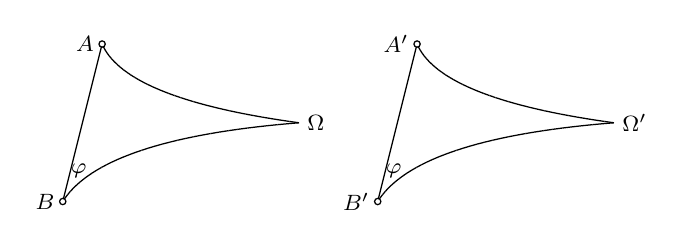
\begin{tikzpicture}
            % \clip (0,0) rectangle (14.000000,10.000000);
            {\footnotesize
            
            % Drawing segment A B
            \draw [line width=0.016cm] (2.490299,3.961194) -- (2.009701,2.038806);%
            
            % Drawing Bezier curve A Y \Omega
            \draw [line width=0.016cm] (2.518133,3.961420) -- (2.517014,3.963799);%
            \draw [line width=0.016cm] (2.539198,3.923457) -- (2.518133,3.961420);%
            \draw [line width=0.016cm] (2.563194,3.886111) -- (2.539198,3.923457);%
            \draw [line width=0.016cm] (2.590123,3.849383) -- (2.563194,3.886111);%
            \draw [line width=0.016cm] (2.619985,3.813272) -- (2.590123,3.849383);%
            \draw [line width=0.016cm] (2.652778,3.777778) -- (2.619985,3.813272);%
            \draw [line width=0.016cm] (2.688503,3.742901) -- (2.652778,3.777778);%
            \draw [line width=0.016cm] (2.727160,3.708642) -- (2.688503,3.742901);%
            \draw [line width=0.016cm] (2.768750,3.675000) -- (2.727160,3.708642);%
            \draw [line width=0.016cm] (2.813272,3.641975) -- (2.768750,3.675000);%
            \draw [line width=0.016cm] (2.860725,3.609568) -- (2.813272,3.641975);%
            \draw [line width=0.016cm] (2.911111,3.577778) -- (2.860725,3.609568);%
            \draw [line width=0.016cm] (2.964429,3.546605) -- (2.911111,3.577778);%
            \draw [line width=0.016cm] (3.020679,3.516049) -- (2.964429,3.546605);%
            \draw [line width=0.016cm] (3.079861,3.486111) -- (3.020679,3.516049);%
            \draw [line width=0.016cm] (3.141975,3.456790) -- (3.079861,3.486111);%
            \draw [line width=0.016cm] (3.207022,3.428086) -- (3.141975,3.456790);%
            \draw [line width=0.016cm] (3.275000,3.400000) -- (3.207022,3.428086);%
            \draw [line width=0.016cm] (3.345910,3.372531) -- (3.275000,3.400000);%
            \draw [line width=0.016cm] (3.419753,3.345679) -- (3.345910,3.372531);%
            \draw [line width=0.016cm] (3.496528,3.319444) -- (3.419753,3.345679);%
            \draw [line width=0.016cm] (3.576235,3.293827) -- (3.496528,3.319444);%
            \draw [line width=0.016cm] (3.658873,3.268827) -- (3.576235,3.293827);%
            \draw [line width=0.016cm] (3.744444,3.244444) -- (3.658873,3.268827);%
            \draw [line width=0.016cm] (3.832948,3.220679) -- (3.744444,3.244444);%
            \draw [line width=0.016cm] (3.924383,3.197531) -- (3.832948,3.220679);%
            \draw [line width=0.016cm] (4.018750,3.175000) -- (3.924383,3.197531);%
            \draw [line width=0.016cm] (4.116049,3.153086) -- (4.018750,3.175000);%
            \draw [line width=0.016cm] (4.216281,3.131790) -- (4.116049,3.153086);%
            \draw [line width=0.016cm] (4.319444,3.111111) -- (4.216281,3.131790);%
            \draw [line width=0.016cm] (4.425540,3.091049) -- (4.319444,3.111111);%
            \draw [line width=0.016cm] (4.534568,3.071605) -- (4.425540,3.091049);%
            \draw [line width=0.016cm] (4.646528,3.052778) -- (4.534568,3.071605);%
            \draw [line width=0.016cm] (4.761420,3.034568) -- (4.646528,3.052778);%
            \draw [line width=0.016cm] (4.879244,3.016975) -- (4.761420,3.034568);%
            \draw [line width=0.016cm] (5.000000,3.000000) -- (4.879244,3.016975);%
            
            % Drawing Bezier curve B X \Omega
            \draw [line width=0.016cm] (2.029321,2.043981) -- (2.022188,2.033282);%
            \draw [line width=0.016cm] (2.061728,2.087037) -- (2.029321,2.043981);%
            \draw [line width=0.016cm] (2.097222,2.129167) -- (2.061728,2.087037);%
            \draw [line width=0.016cm] (2.135802,2.170370) -- (2.097222,2.129167);%
            \draw [line width=0.016cm] (2.177469,2.210648) -- (2.135802,2.170370);%
            \draw [line width=0.016cm] (2.222222,2.250000) -- (2.177469,2.210648);%
            \draw [line width=0.016cm] (2.270062,2.288426) -- (2.222222,2.250000);%
            \draw [line width=0.016cm] (2.320988,2.325926) -- (2.270062,2.288426);%
            \draw [line width=0.016cm] (2.375000,2.362500) -- (2.320988,2.325926);%
            \draw [line width=0.016cm] (2.432099,2.398148) -- (2.375000,2.362500);%
            \draw [line width=0.016cm] (2.492284,2.432870) -- (2.432099,2.398148);%
            \draw [line width=0.016cm] (2.555556,2.466667) -- (2.492284,2.432870);%
            \draw [line width=0.016cm] (2.621914,2.499537) -- (2.555556,2.466667);%
            \draw [line width=0.016cm] (2.691358,2.531481) -- (2.621914,2.499537);%
            \draw [line width=0.016cm] (2.763889,2.562500) -- (2.691358,2.531481);%
            \draw [line width=0.016cm] (2.839506,2.592593) -- (2.763889,2.562500);%
            \draw [line width=0.016cm] (2.918210,2.621759) -- (2.839506,2.592593);%
            \draw [line width=0.016cm] (3.000000,2.650000) -- (2.918210,2.621759);%
            \draw [line width=0.016cm] (3.084877,2.677315) -- (3.000000,2.650000);%
            \draw [line width=0.016cm] (3.172840,2.703704) -- (3.084877,2.677315);%
            \draw [line width=0.016cm] (3.263889,2.729167) -- (3.172840,2.703704);%
            \draw [line width=0.016cm] (3.358025,2.753704) -- (3.263889,2.729167);%
            \draw [line width=0.016cm] (3.455247,2.777315) -- (3.358025,2.753704);%
            \draw [line width=0.016cm] (3.555556,2.800000) -- (3.455247,2.777315);%
            \draw [line width=0.016cm] (3.658951,2.821759) -- (3.555556,2.800000);%
            \draw [line width=0.016cm] (3.765432,2.842593) -- (3.658951,2.821759);%
            \draw [line width=0.016cm] (3.875000,2.862500) -- (3.765432,2.842593);%
            \draw [line width=0.016cm] (3.987654,2.881481) -- (3.875000,2.862500);%
            \draw [line width=0.016cm] (4.103395,2.899537) -- (3.987654,2.881481);%
            \draw [line width=0.016cm] (4.222222,2.916667) -- (4.103395,2.899537);%
            \draw [line width=0.016cm] (4.344136,2.932870) -- (4.222222,2.916667);%
            \draw [line width=0.016cm] (4.469136,2.948148) -- (4.344136,2.932870);%
            \draw [line width=0.016cm] (4.597222,2.962500) -- (4.469136,2.948148);%
            \draw [line width=0.016cm] (4.728395,2.975926) -- (4.597222,2.962500);%
            \draw [line width=0.016cm] (4.862654,2.988426) -- (4.728395,2.975926);%
            \draw [line width=0.016cm] (5.000000,3.000000) -- (4.862654,2.988426);%
            
            % Marking point A by circle
            \draw [line width=0.016cm] (2.500000,4.000000) circle (0.040000);%
            \draw (2.500000,4.000000) node [anchor=east] { $A$ };%
            
            % Marking point B by circle
            \draw [line width=0.016cm] (2.000000,2.000000) circle (0.040000);%
            \draw (2.000000,2.000000) node [anchor=east] { $B$ };%
            
            % Marking point \Omega
            \draw (5.000000,3.000000) node [anchor=west] { $\Omega$ };%
            
            % Drawing segment A' B'
            \draw [line width=0.016cm] (6.490299,3.961194) -- (6.009701,2.038806);%
            
            % Drawing Bezier curve A' Y' \Omega'
            \draw [line width=0.016cm] (6.518133,3.961420) -- (6.517014,3.963799);%
            \draw [line width=0.016cm] (6.539198,3.923457) -- (6.518133,3.961420);%
            \draw [line width=0.016cm] (6.563194,3.886111) -- (6.539198,3.923457);%
            \draw [line width=0.016cm] (6.590123,3.849383) -- (6.563194,3.886111);%
            \draw [line width=0.016cm] (6.619985,3.813272) -- (6.590123,3.849383);%
            \draw [line width=0.016cm] (6.652778,3.777778) -- (6.619985,3.813272);%
            \draw [line width=0.016cm] (6.688503,3.742901) -- (6.652778,3.777778);%
            \draw [line width=0.016cm] (6.727160,3.708642) -- (6.688503,3.742901);%
            \draw [line width=0.016cm] (6.768750,3.675000) -- (6.727160,3.708642);%
            \draw [line width=0.016cm] (6.813272,3.641975) -- (6.768750,3.675000);%
            \draw [line width=0.016cm] (6.860725,3.609568) -- (6.813272,3.641975);%
            \draw [line width=0.016cm] (6.911111,3.577778) -- (6.860725,3.609568);%
            \draw [line width=0.016cm] (6.964429,3.546605) -- (6.911111,3.577778);%
            \draw [line width=0.016cm] (7.020679,3.516049) -- (6.964429,3.546605);%
            \draw [line width=0.016cm] (7.079861,3.486111) -- (7.020679,3.516049);%
            \draw [line width=0.016cm] (7.141975,3.456790) -- (7.079861,3.486111);%
            \draw [line width=0.016cm] (7.207022,3.428086) -- (7.141975,3.456790);%
            \draw [line width=0.016cm] (7.275000,3.400000) -- (7.207022,3.428086);%
            \draw [line width=0.016cm] (7.345910,3.372531) -- (7.275000,3.400000);%
            \draw [line width=0.016cm] (7.419753,3.345679) -- (7.345910,3.372531);%
            \draw [line width=0.016cm] (7.496528,3.319444) -- (7.419753,3.345679);%
            \draw [line width=0.016cm] (7.576235,3.293827) -- (7.496528,3.319444);%
            \draw [line width=0.016cm] (7.658873,3.268827) -- (7.576235,3.293827);%
            \draw [line width=0.016cm] (7.744444,3.244444) -- (7.658873,3.268827);%
            \draw [line width=0.016cm] (7.832948,3.220679) -- (7.744444,3.244444);%
            \draw [line width=0.016cm] (7.924383,3.197531) -- (7.832948,3.220679);%
            \draw [line width=0.016cm] (8.018750,3.175000) -- (7.924383,3.197531);%
            \draw [line width=0.016cm] (8.116049,3.153086) -- (8.018750,3.175000);%
            \draw [line width=0.016cm] (8.216281,3.131790) -- (8.116049,3.153086);%
            \draw [line width=0.016cm] (8.319444,3.111111) -- (8.216281,3.131790);%
            \draw [line width=0.016cm] (8.425540,3.091049) -- (8.319444,3.111111);%
            \draw [line width=0.016cm] (8.534568,3.071605) -- (8.425540,3.091049);%
            \draw [line width=0.016cm] (8.646528,3.052778) -- (8.534568,3.071605);%
            \draw [line width=0.016cm] (8.761420,3.034568) -- (8.646528,3.052778);%
            \draw [line width=0.016cm] (8.879244,3.016975) -- (8.761420,3.034568);%
            \draw [line width=0.016cm] (9.000000,3.000000) -- (8.879244,3.016975);%
            
            % Drawing Bezier curve B' X' \Omega'
            \draw [line width=0.016cm] (6.029321,2.043981) -- (6.022188,2.033282);%
            \draw [line width=0.016cm] (6.061728,2.087037) -- (6.029321,2.043981);%
            \draw [line width=0.016cm] (6.097222,2.129167) -- (6.061728,2.087037);%
            \draw [line width=0.016cm] (6.135802,2.170370) -- (6.097222,2.129167);%
            \draw [line width=0.016cm] (6.177469,2.210648) -- (6.135802,2.170370);%
            \draw [line width=0.016cm] (6.222222,2.250000) -- (6.177469,2.210648);%
            \draw [line width=0.016cm] (6.270062,2.288426) -- (6.222222,2.250000);%
            \draw [line width=0.016cm] (6.320988,2.325926) -- (6.270062,2.288426);%
            \draw [line width=0.016cm] (6.375000,2.362500) -- (6.320988,2.325926);%
            \draw [line width=0.016cm] (6.432099,2.398148) -- (6.375000,2.362500);%
            \draw [line width=0.016cm] (6.492284,2.432870) -- (6.432099,2.398148);%
            \draw [line width=0.016cm] (6.555556,2.466667) -- (6.492284,2.432870);%
            \draw [line width=0.016cm] (6.621914,2.499537) -- (6.555556,2.466667);%
            \draw [line width=0.016cm] (6.691358,2.531481) -- (6.621914,2.499537);%
            \draw [line width=0.016cm] (6.763889,2.562500) -- (6.691358,2.531481);%
            \draw [line width=0.016cm] (6.839506,2.592593) -- (6.763889,2.562500);%
            \draw [line width=0.016cm] (6.918210,2.621759) -- (6.839506,2.592593);%
            \draw [line width=0.016cm] (7.000000,2.650000) -- (6.918210,2.621759);%
            \draw [line width=0.016cm] (7.084877,2.677315) -- (7.000000,2.650000);%
            \draw [line width=0.016cm] (7.172840,2.703704) -- (7.084877,2.677315);%
            \draw [line width=0.016cm] (7.263889,2.729167) -- (7.172840,2.703704);%
            \draw [line width=0.016cm] (7.358025,2.753704) -- (7.263889,2.729167);%
            \draw [line width=0.016cm] (7.455247,2.777315) -- (7.358025,2.753704);%
            \draw [line width=0.016cm] (7.555556,2.800000) -- (7.455247,2.777315);%
            \draw [line width=0.016cm] (7.658951,2.821759) -- (7.555556,2.800000);%
            \draw [line width=0.016cm] (7.765432,2.842593) -- (7.658951,2.821759);%
            \draw [line width=0.016cm] (7.875000,2.862500) -- (7.765432,2.842593);%
            \draw [line width=0.016cm] (7.987654,2.881481) -- (7.875000,2.862500);%
            \draw [line width=0.016cm] (8.103395,2.899537) -- (7.987654,2.881481);%
            \draw [line width=0.016cm] (8.222222,2.916667) -- (8.103395,2.899537);%
            \draw [line width=0.016cm] (8.344136,2.932870) -- (8.222222,2.916667);%
            \draw [line width=0.016cm] (8.469136,2.948148) -- (8.344136,2.932870);%
            \draw [line width=0.016cm] (8.597222,2.962500) -- (8.469136,2.948148);%
            \draw [line width=0.016cm] (8.728395,2.975926) -- (8.597222,2.962500);%
            \draw [line width=0.016cm] (8.862654,2.988426) -- (8.728395,2.975926);%
            \draw [line width=0.016cm] (9.000000,3.000000) -- (8.862654,2.988426);%
            
            % Marking point A' by circle
            \draw [line width=0.016cm] (6.500000,4.000000) circle (0.040000);%
            \draw (6.500000,4.000000) node [anchor=east] { $A'$ };%
            
            % Marking point B' by circle
            \draw [line width=0.016cm] (6.000000,2.000000) circle (0.040000);%
            \draw (6.000000,2.000000) node [anchor=east] { $B'$ };%
            
            % Marking point \Omega'
            \draw (9.000000,3.000000) node [anchor=west] { $\Omega'$ };%
            
            % Marking point \varphi
            \draw (2.000000,2.200000) node [anchor=south west] { $\varphi$ };%
            
            % Marking point \varphi
            \draw (6.000000,2.200000) node [anchor=south west] { $\varphi$ };%
            }
        \end{tikzpicture}
        
        \begin{dokaz}
            \\ ($\Rightarrow$):
            \\ Naj bo $AB\cong A'B'$. Recimo, da je $\angle BA\Omega \ncong \angle B'A'\Omega'$, torej naj bo $\angle BA\Omega > \angle B'A'\Omega'$. 
            \\ 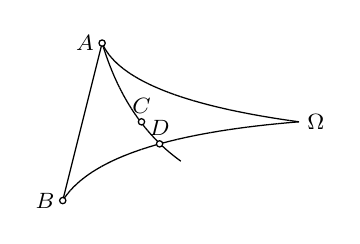
\begin{tikzpicture}
                    % \clip (0,0) rectangle (14.000000,10.000000);
                    {\footnotesize
                    
                    % Drawing segment A B
                    \draw [line width=0.016cm] (2.490299,3.961194) -- (2.009701,2.038806);%
                    
                    % Drawing Bezier curve A Y \Omega
                    \draw [line width=0.016cm] (2.518133,3.961420) -- (2.517014,3.963799);%
                    \draw [line width=0.016cm] (2.539198,3.923457) -- (2.518133,3.961420);%
                    \draw [line width=0.016cm] (2.563194,3.886111) -- (2.539198,3.923457);%
                    \draw [line width=0.016cm] (2.590123,3.849383) -- (2.563194,3.886111);%
                    \draw [line width=0.016cm] (2.619985,3.813272) -- (2.590123,3.849383);%
                    \draw [line width=0.016cm] (2.652778,3.777778) -- (2.619985,3.813272);%
                    \draw [line width=0.016cm] (2.688503,3.742901) -- (2.652778,3.777778);%
                    \draw [line width=0.016cm] (2.727160,3.708642) -- (2.688503,3.742901);%
                    \draw [line width=0.016cm] (2.768750,3.675000) -- (2.727160,3.708642);%
                    \draw [line width=0.016cm] (2.813272,3.641975) -- (2.768750,3.675000);%
                    \draw [line width=0.016cm] (2.860725,3.609568) -- (2.813272,3.641975);%
                    \draw [line width=0.016cm] (2.911111,3.577778) -- (2.860725,3.609568);%
                    \draw [line width=0.016cm] (2.964429,3.546605) -- (2.911111,3.577778);%
                    \draw [line width=0.016cm] (3.020679,3.516049) -- (2.964429,3.546605);%
                    \draw [line width=0.016cm] (3.079861,3.486111) -- (3.020679,3.516049);%
                    \draw [line width=0.016cm] (3.141975,3.456790) -- (3.079861,3.486111);%
                    \draw [line width=0.016cm] (3.207022,3.428086) -- (3.141975,3.456790);%
                    \draw [line width=0.016cm] (3.275000,3.400000) -- (3.207022,3.428086);%
                    \draw [line width=0.016cm] (3.345910,3.372531) -- (3.275000,3.400000);%
                    \draw [line width=0.016cm] (3.419753,3.345679) -- (3.345910,3.372531);%
                    \draw [line width=0.016cm] (3.496528,3.319444) -- (3.419753,3.345679);%
                    \draw [line width=0.016cm] (3.576235,3.293827) -- (3.496528,3.319444);%
                    \draw [line width=0.016cm] (3.658873,3.268827) -- (3.576235,3.293827);%
                    \draw [line width=0.016cm] (3.744444,3.244444) -- (3.658873,3.268827);%
                    \draw [line width=0.016cm] (3.832948,3.220679) -- (3.744444,3.244444);%
                    \draw [line width=0.016cm] (3.924383,3.197531) -- (3.832948,3.220679);%
                    \draw [line width=0.016cm] (4.018750,3.175000) -- (3.924383,3.197531);%
                    \draw [line width=0.016cm] (4.116049,3.153086) -- (4.018750,3.175000);%
                    \draw [line width=0.016cm] (4.216281,3.131790) -- (4.116049,3.153086);%
                    \draw [line width=0.016cm] (4.319444,3.111111) -- (4.216281,3.131790);%
                    \draw [line width=0.016cm] (4.425540,3.091049) -- (4.319444,3.111111);%
                    \draw [line width=0.016cm] (4.534568,3.071605) -- (4.425540,3.091049);%
                    \draw [line width=0.016cm] (4.646528,3.052778) -- (4.534568,3.071605);%
                    \draw [line width=0.016cm] (4.761420,3.034568) -- (4.646528,3.052778);%
                    \draw [line width=0.016cm] (4.879244,3.016975) -- (4.761420,3.034568);%
                    \draw [line width=0.016cm] (5.000000,3.000000) -- (4.879244,3.016975);%
                    
                    % Drawing Bezier curve B X \Omega
                    \draw [line width=0.016cm] (2.029321,2.043981) -- (2.022188,2.033282);%
                    \draw [line width=0.016cm] (2.061728,2.087037) -- (2.029321,2.043981);%
                    \draw [line width=0.016cm] (2.097222,2.129167) -- (2.061728,2.087037);%
                    \draw [line width=0.016cm] (2.135802,2.170370) -- (2.097222,2.129167);%
                    \draw [line width=0.016cm] (2.177469,2.210648) -- (2.135802,2.170370);%
                    \draw [line width=0.016cm] (2.222222,2.250000) -- (2.177469,2.210648);%
                    \draw [line width=0.016cm] (2.270062,2.288426) -- (2.222222,2.250000);%
                    \draw [line width=0.016cm] (2.320988,2.325926) -- (2.270062,2.288426);%
                    \draw [line width=0.016cm] (2.375000,2.362500) -- (2.320988,2.325926);%
                    \draw [line width=0.016cm] (2.432099,2.398148) -- (2.375000,2.362500);%
                    \draw [line width=0.016cm] (2.492284,2.432870) -- (2.432099,2.398148);%
                    \draw [line width=0.016cm] (2.555556,2.466667) -- (2.492284,2.432870);%
                    \draw [line width=0.016cm] (2.621914,2.499537) -- (2.555556,2.466667);%
                    \draw [line width=0.016cm] (2.691358,2.531481) -- (2.621914,2.499537);%
                    \draw [line width=0.016cm] (2.763889,2.562500) -- (2.691358,2.531481);%
                    \draw [line width=0.016cm] (2.839506,2.592593) -- (2.763889,2.562500);%
                    \draw [line width=0.016cm] (2.918210,2.621759) -- (2.839506,2.592593);%
                    \draw [line width=0.016cm] (3.000000,2.650000) -- (2.918210,2.621759);%
                    \draw [line width=0.016cm] (3.084877,2.677315) -- (3.000000,2.650000);%
                    \draw [line width=0.016cm] (3.172840,2.703704) -- (3.084877,2.677315);%
                    \draw [line width=0.016cm] (3.191560,2.708939) -- (3.172840,2.703704);%
                    \draw [line width=0.016cm] (3.358025,2.753704) -- (3.268624,2.730401);%
                    \draw [line width=0.016cm] (3.455247,2.777315) -- (3.358025,2.753704);%
                    \draw [line width=0.016cm] (3.555556,2.800000) -- (3.455247,2.777315);%
                    \draw [line width=0.016cm] (3.658951,2.821759) -- (3.555556,2.800000);%
                    \draw [line width=0.016cm] (3.765432,2.842593) -- (3.658951,2.821759);%
                    \draw [line width=0.016cm] (3.875000,2.862500) -- (3.765432,2.842593);%
                    \draw [line width=0.016cm] (3.987654,2.881481) -- (3.875000,2.862500);%
                    \draw [line width=0.016cm] (4.103395,2.899537) -- (3.987654,2.881481);%
                    \draw [line width=0.016cm] (4.222222,2.916667) -- (4.103395,2.899537);%
                    \draw [line width=0.016cm] (4.344136,2.932870) -- (4.222222,2.916667);%
                    \draw [line width=0.016cm] (4.469136,2.948148) -- (4.344136,2.932870);%
                    \draw [line width=0.016cm] (4.597222,2.962500) -- (4.469136,2.948148);%
                    \draw [line width=0.016cm] (4.728395,2.975926) -- (4.597222,2.962500);%
                    \draw [line width=0.016cm] (4.862654,2.988426) -- (4.728395,2.975926);%
                    \draw [line width=0.016cm] (5.000000,3.000000) -- (4.862654,2.988426);%
                    
                    % Drawing Bezier curve A Z V
                    \draw [line width=0.016cm] (2.516975,3.944830) -- (2.511763,3.961769);%
                    \draw [line width=0.016cm] (2.534568,3.890432) -- (2.516975,3.944830);%
                    \draw [line width=0.016cm] (2.552778,3.836806) -- (2.534568,3.890432);%
                    \draw [line width=0.016cm] (2.571605,3.783951) -- (2.552778,3.836806);%
                    \draw [line width=0.016cm] (2.591049,3.731867) -- (2.571605,3.783951);%
                    \draw [line width=0.016cm] (2.611111,3.680556) -- (2.591049,3.731867);%
                    \draw [line width=0.016cm] (2.631790,3.630015) -- (2.611111,3.680556);%
                    \draw [line width=0.016cm] (2.653086,3.580247) -- (2.631790,3.630015);%
                    \draw [line width=0.016cm] (2.675000,3.531250) -- (2.653086,3.580247);%
                    \draw [line width=0.016cm] (2.697531,3.483025) -- (2.675000,3.531250);%
                    \draw [line width=0.016cm] (2.720679,3.435571) -- (2.697531,3.483025);%
                    \draw [line width=0.016cm] (2.744444,3.388889) -- (2.720679,3.435571);%
                    \draw [line width=0.016cm] (2.768827,3.342978) -- (2.744444,3.388889);%
                    \draw [line width=0.016cm] (2.793827,3.297840) -- (2.768827,3.342978);%
                    \draw [line width=0.016cm] (2.819444,3.253472) -- (2.793827,3.297840);%
                    \draw [line width=0.016cm] (2.845679,3.209877) -- (2.819444,3.253472);%
                    \draw [line width=0.016cm] (2.872531,3.167052) -- (2.845679,3.209877);%
                    \draw [line width=0.016cm] (2.900000,3.125000) -- (2.872531,3.167052);%
                    \draw [line width=0.016cm] (2.928086,3.083719) -- (2.900000,3.125000);%
                    \draw [line width=0.016cm] (2.956790,3.043210) -- (2.928086,3.083719);%
                    \draw [line width=0.016cm] (2.969542,3.025928) -- (2.956790,3.043210);%
                    \draw [line width=0.016cm] (3.046605,2.926312) -- (3.016723,2.963664);%
                    \draw [line width=0.016cm] (3.077778,2.888889) -- (3.046605,2.926312);%
                    \draw [line width=0.016cm] (3.109568,2.852238) -- (3.077778,2.888889);%
                    \draw [line width=0.016cm] (3.141975,2.816358) -- (3.109568,2.852238);%
                    \draw [line width=0.016cm] (3.175000,2.781250) -- (3.141975,2.816358);%
                    \draw [line width=0.016cm] (3.204675,2.750962) -- (3.175000,2.781250);%
                    \draw [line width=0.016cm] (3.277778,2.680556) -- (3.261730,2.695644);%
                    \draw [line width=0.016cm] (3.313272,2.648534) -- (3.277778,2.680556);%
                    \draw [line width=0.016cm] (3.349383,2.617284) -- (3.313272,2.648534);%
                    \draw [line width=0.016cm] (3.386111,2.586806) -- (3.349383,2.617284);%
                    \draw [line width=0.016cm] (3.423457,2.557099) -- (3.386111,2.586806);%
                    \draw [line width=0.016cm] (3.461420,2.528164) -- (3.423457,2.557099);%
                    \draw [line width=0.016cm] (3.500000,2.500000) -- (3.461420,2.528164);%
                    
                    % Marking point A by circle
                    \draw [line width=0.016cm] (2.500000,4.000000) circle (0.040000);%
                    \draw (2.500000,4.000000) node [anchor=east] { $A$ };%
                    
                    % Marking point B by circle
                    \draw [line width=0.016cm] (2.000000,2.000000) circle (0.040000);%
                    \draw (2.000000,2.000000) node [anchor=east] { $B$ };%
                    
                    % Marking point \Omega
                    \draw (5.000000,3.000000) node [anchor=west] { $\Omega$ };%
                    
                    % Marking point D by circle
                    \draw [line width=0.016cm] (3.230000,2.720000) circle (0.040000);%
                    \draw (3.230000,2.720000) node [anchor=south] { $D$ };%
                    
                    % Marking point C by circle
                    \draw [line width=0.016cm] (3.000000,3.000000) circle (0.040000);%
                    \draw (3.000000,3.000000) node [anchor=south] { $C$ };%
                    }
                \end{tikzpicture}                
            \\ Potem obstaja točka $C$ znotraj kota $\angle BA\Omega$, da je $\angle BAC\cong\angle B'A'\Omega'$. Ker je poltrak $\overrightarrow{AC}$ znotraj kota $\angle BA\Omega$ in je $\overrightarrow{A\Omega}$ asimptotičen poltrak k poltraku $\overrightarrow{B\Omega}$, potem velja, da $\overrightarrow{AC}$ seka $\overrightarrow{B\Omega}$ v točki $D$. 
            \\ 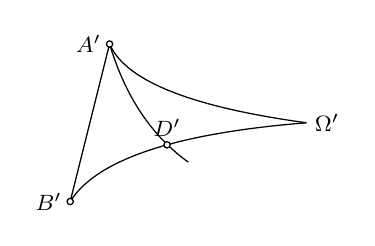
\begin{tikzpicture}
                    % \clip (0,0) rectangle (14.000000,10.000000);
                    {\footnotesize
                    
                    % Drawing segment A' B'
                    \draw [line width=0.016cm] (2.490299,3.961194) -- (2.009701,2.038806);%
                    
                    % Drawing Bezier curve A' Y \Omega'
                    \draw [line width=0.016cm] (2.518133,3.961420) -- (2.517014,3.963799);%
                    \draw [line width=0.016cm] (2.539198,3.923457) -- (2.518133,3.961420);%
                    \draw [line width=0.016cm] (2.563194,3.886111) -- (2.539198,3.923457);%
                    \draw [line width=0.016cm] (2.590123,3.849383) -- (2.563194,3.886111);%
                    \draw [line width=0.016cm] (2.619985,3.813272) -- (2.590123,3.849383);%
                    \draw [line width=0.016cm] (2.652778,3.777778) -- (2.619985,3.813272);%
                    \draw [line width=0.016cm] (2.688503,3.742901) -- (2.652778,3.777778);%
                    \draw [line width=0.016cm] (2.727160,3.708642) -- (2.688503,3.742901);%
                    \draw [line width=0.016cm] (2.768750,3.675000) -- (2.727160,3.708642);%
                    \draw [line width=0.016cm] (2.813272,3.641975) -- (2.768750,3.675000);%
                    \draw [line width=0.016cm] (2.860725,3.609568) -- (2.813272,3.641975);%
                    \draw [line width=0.016cm] (2.911111,3.577778) -- (2.860725,3.609568);%
                    \draw [line width=0.016cm] (2.964429,3.546605) -- (2.911111,3.577778);%
                    \draw [line width=0.016cm] (3.020679,3.516049) -- (2.964429,3.546605);%
                    \draw [line width=0.016cm] (3.079861,3.486111) -- (3.020679,3.516049);%
                    \draw [line width=0.016cm] (3.141975,3.456790) -- (3.079861,3.486111);%
                    \draw [line width=0.016cm] (3.207022,3.428086) -- (3.141975,3.456790);%
                    \draw [line width=0.016cm] (3.275000,3.400000) -- (3.207022,3.428086);%
                    \draw [line width=0.016cm] (3.345910,3.372531) -- (3.275000,3.400000);%
                    \draw [line width=0.016cm] (3.419753,3.345679) -- (3.345910,3.372531);%
                    \draw [line width=0.016cm] (3.496528,3.319444) -- (3.419753,3.345679);%
                    \draw [line width=0.016cm] (3.576235,3.293827) -- (3.496528,3.319444);%
                    \draw [line width=0.016cm] (3.658873,3.268827) -- (3.576235,3.293827);%
                    \draw [line width=0.016cm] (3.744444,3.244444) -- (3.658873,3.268827);%
                    \draw [line width=0.016cm] (3.832948,3.220679) -- (3.744444,3.244444);%
                    \draw [line width=0.016cm] (3.924383,3.197531) -- (3.832948,3.220679);%
                    \draw [line width=0.016cm] (4.018750,3.175000) -- (3.924383,3.197531);%
                    \draw [line width=0.016cm] (4.116049,3.153086) -- (4.018750,3.175000);%
                    \draw [line width=0.016cm] (4.216281,3.131790) -- (4.116049,3.153086);%
                    \draw [line width=0.016cm] (4.319444,3.111111) -- (4.216281,3.131790);%
                    \draw [line width=0.016cm] (4.425540,3.091049) -- (4.319444,3.111111);%
                    \draw [line width=0.016cm] (4.534568,3.071605) -- (4.425540,3.091049);%
                    \draw [line width=0.016cm] (4.646528,3.052778) -- (4.534568,3.071605);%
                    \draw [line width=0.016cm] (4.761420,3.034568) -- (4.646528,3.052778);%
                    \draw [line width=0.016cm] (4.879244,3.016975) -- (4.761420,3.034568);%
                    \draw [line width=0.016cm] (5.000000,3.000000) -- (4.879244,3.016975);%
                    
                    % Drawing Bezier curve B' X \Omega'
                    \draw [line width=0.016cm] (2.029321,2.043981) -- (2.022188,2.033282);%
                    \draw [line width=0.016cm] (2.061728,2.087037) -- (2.029321,2.043981);%
                    \draw [line width=0.016cm] (2.097222,2.129167) -- (2.061728,2.087037);%
                    \draw [line width=0.016cm] (2.135802,2.170370) -- (2.097222,2.129167);%
                    \draw [line width=0.016cm] (2.177469,2.210648) -- (2.135802,2.170370);%
                    \draw [line width=0.016cm] (2.222222,2.250000) -- (2.177469,2.210648);%
                    \draw [line width=0.016cm] (2.270062,2.288426) -- (2.222222,2.250000);%
                    \draw [line width=0.016cm] (2.320988,2.325926) -- (2.270062,2.288426);%
                    \draw [line width=0.016cm] (2.375000,2.362500) -- (2.320988,2.325926);%
                    \draw [line width=0.016cm] (2.432099,2.398148) -- (2.375000,2.362500);%
                    \draw [line width=0.016cm] (2.492284,2.432870) -- (2.432099,2.398148);%
                    \draw [line width=0.016cm] (2.555556,2.466667) -- (2.492284,2.432870);%
                    \draw [line width=0.016cm] (2.621914,2.499537) -- (2.555556,2.466667);%
                    \draw [line width=0.016cm] (2.691358,2.531481) -- (2.621914,2.499537);%
                    \draw [line width=0.016cm] (2.763889,2.562500) -- (2.691358,2.531481);%
                    \draw [line width=0.016cm] (2.839506,2.592593) -- (2.763889,2.562500);%
                    \draw [line width=0.016cm] (2.918210,2.621759) -- (2.839506,2.592593);%
                    \draw [line width=0.016cm] (3.000000,2.650000) -- (2.918210,2.621759);%
                    \draw [line width=0.016cm] (3.084877,2.677315) -- (3.000000,2.650000);%
                    \draw [line width=0.016cm] (3.172840,2.703704) -- (3.084877,2.677315);%
                    \draw [line width=0.016cm] (3.191560,2.708939) -- (3.172840,2.703704);%
                    \draw [line width=0.016cm] (3.358025,2.753704) -- (3.268624,2.730401);%
                    \draw [line width=0.016cm] (3.455247,2.777315) -- (3.358025,2.753704);%
                    \draw [line width=0.016cm] (3.555556,2.800000) -- (3.455247,2.777315);%
                    \draw [line width=0.016cm] (3.658951,2.821759) -- (3.555556,2.800000);%
                    \draw [line width=0.016cm] (3.765432,2.842593) -- (3.658951,2.821759);%
                    \draw [line width=0.016cm] (3.875000,2.862500) -- (3.765432,2.842593);%
                    \draw [line width=0.016cm] (3.987654,2.881481) -- (3.875000,2.862500);%
                    \draw [line width=0.016cm] (4.103395,2.899537) -- (3.987654,2.881481);%
                    \draw [line width=0.016cm] (4.222222,2.916667) -- (4.103395,2.899537);%
                    \draw [line width=0.016cm] (4.344136,2.932870) -- (4.222222,2.916667);%
                    \draw [line width=0.016cm] (4.469136,2.948148) -- (4.344136,2.932870);%
                    \draw [line width=0.016cm] (4.597222,2.962500) -- (4.469136,2.948148);%
                    \draw [line width=0.016cm] (4.728395,2.975926) -- (4.597222,2.962500);%
                    \draw [line width=0.016cm] (4.862654,2.988426) -- (4.728395,2.975926);%
                    \draw [line width=0.016cm] (5.000000,3.000000) -- (4.862654,2.988426);%
                    
                    % Drawing Bezier curve A' Z V
                    \draw [line width=0.016cm] (2.516975,3.944830) -- (2.511763,3.961769);%
                    \draw [line width=0.016cm] (2.534568,3.890432) -- (2.516975,3.944830);%
                    \draw [line width=0.016cm] (2.552778,3.836806) -- (2.534568,3.890432);%
                    \draw [line width=0.016cm] (2.571605,3.783951) -- (2.552778,3.836806);%
                    \draw [line width=0.016cm] (2.591049,3.731867) -- (2.571605,3.783951);%
                    \draw [line width=0.016cm] (2.611111,3.680556) -- (2.591049,3.731867);%
                    \draw [line width=0.016cm] (2.631790,3.630015) -- (2.611111,3.680556);%
                    \draw [line width=0.016cm] (2.653086,3.580247) -- (2.631790,3.630015);%
                    \draw [line width=0.016cm] (2.675000,3.531250) -- (2.653086,3.580247);%
                    \draw [line width=0.016cm] (2.697531,3.483025) -- (2.675000,3.531250);%
                    \draw [line width=0.016cm] (2.720679,3.435571) -- (2.697531,3.483025);%
                    \draw [line width=0.016cm] (2.744444,3.388889) -- (2.720679,3.435571);%
                    \draw [line width=0.016cm] (2.768827,3.342978) -- (2.744444,3.388889);%
                    \draw [line width=0.016cm] (2.793827,3.297840) -- (2.768827,3.342978);%
                    \draw [line width=0.016cm] (2.819444,3.253472) -- (2.793827,3.297840);%
                    \draw [line width=0.016cm] (2.845679,3.209877) -- (2.819444,3.253472);%
                    \draw [line width=0.016cm] (2.872531,3.167052) -- (2.845679,3.209877);%
                    \draw [line width=0.016cm] (2.900000,3.125000) -- (2.872531,3.167052);%
                    \draw [line width=0.016cm] (2.928086,3.083719) -- (2.900000,3.125000);%
                    \draw [line width=0.016cm] (2.956790,3.043210) -- (2.928086,3.083719);%
                    \draw [line width=0.016cm] (2.986111,3.003472) -- (2.956790,3.043210);%
                    \draw [line width=0.016cm] (3.016049,2.964506) -- (2.986111,3.003472);%
                    \draw [line width=0.016cm] (3.046605,2.926312) -- (3.016049,2.964506);%
                    \draw [line width=0.016cm] (3.077778,2.888889) -- (3.046605,2.926312);%
                    \draw [line width=0.016cm] (3.109568,2.852238) -- (3.077778,2.888889);%
                    \draw [line width=0.016cm] (3.141975,2.816358) -- (3.109568,2.852238);%
                    \draw [line width=0.016cm] (3.175000,2.781250) -- (3.141975,2.816358);%
                    \draw [line width=0.016cm] (3.204675,2.750962) -- (3.175000,2.781250);%
                    \draw [line width=0.016cm] (3.277778,2.680556) -- (3.261730,2.695644);%
                    \draw [line width=0.016cm] (3.313272,2.648534) -- (3.277778,2.680556);%
                    \draw [line width=0.016cm] (3.349383,2.617284) -- (3.313272,2.648534);%
                    \draw [line width=0.016cm] (3.386111,2.586806) -- (3.349383,2.617284);%
                    \draw [line width=0.016cm] (3.423457,2.557099) -- (3.386111,2.586806);%
                    \draw [line width=0.016cm] (3.461420,2.528164) -- (3.423457,2.557099);%
                    \draw [line width=0.016cm] (3.500000,2.500000) -- (3.461420,2.528164);%
                    
                    % Marking point A' by circle
                    \draw [line width=0.016cm] (2.500000,4.000000) circle (0.040000);%
                    \draw (2.500000,4.000000) node [anchor=east] { $A'$ };%
                    
                    % Marking point B' by circle
                    \draw [line width=0.016cm] (2.000000,2.000000) circle (0.040000);%
                    \draw (2.000000,2.000000) node [anchor=east] { $B'$ };%
                    
                    % Marking point \Omega'
                    \draw (5.000000,3.000000) node [anchor=west] { $\Omega'$ };%
                    
                    % Marking point D' by circle
                    \draw [line width=0.016cm] (3.230000,2.720000) circle (0.040000);%
                    \draw (3.230000,2.720000) node [anchor=south] { $D'$ };%
                    }
                \end{tikzpicture}                
            \\ Potem obstaja točka $D'\in B'\Omega'$ taka, da je $B'D'\cong BD$, in zato poriteriju SKS sledi skladnost trikotnikov $\triangle ABD\cong\triangle A'B'D'$. Iz skladnosti kotov $\angle B'A'D'\cong \angle B'A'\Omega'$ sledi $\overrightarrow{A'D'}>=\overrightarrow{A'\Omega'}$, kar nas privede v protislovje.
            \\ ($\Leftarrow$):
            \\ Naj bo $\angle BA\Omega\cong \angle B'A'\Omega'$. Recimo, da je $AB\ncong A'B'$, torej naj bo $AB>A'B'$. 
            \\ 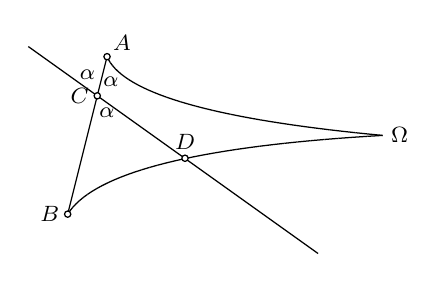
\begin{tikzpicture}
                    % \clip (0,0) rectangle (14.000000,10.000000);
                    {\footnotesize
                    
                    % Drawing segment A B
                    \draw [line width=0.016cm] (2.490299,3.961194) -- (2.385459,3.541836);%
                    \draw [line width=0.016cm] (2.366056,3.464225) -- (2.009701,2.038806);%
                    
                    % Drawing Bezier curve A Y \Omega
                    \draw [line width=0.016cm] (2.518904,3.961420) -- (2.517601,3.964080);%
                    \draw [line width=0.016cm] (2.542284,3.923457) -- (2.518904,3.961420);%
                    \draw [line width=0.016cm] (2.570139,3.886111) -- (2.542284,3.923457);%
                    \draw [line width=0.016cm] (2.602469,3.849383) -- (2.570139,3.886111);%
                    \draw [line width=0.016cm] (2.639275,3.813272) -- (2.602469,3.849383);%
                    \draw [line width=0.016cm] (2.680556,3.777778) -- (2.639275,3.813272);%
                    \draw [line width=0.016cm] (2.726312,3.742901) -- (2.680556,3.777778);%
                    \draw [line width=0.016cm] (2.776543,3.708642) -- (2.726312,3.742901);%
                    \draw [line width=0.016cm] (2.831250,3.675000) -- (2.776543,3.708642);%
                    \draw [line width=0.016cm] (2.890432,3.641975) -- (2.831250,3.675000);%
                    \draw [line width=0.016cm] (2.954090,3.609568) -- (2.890432,3.641975);%
                    \draw [line width=0.016cm] (3.022222,3.577778) -- (2.954090,3.609568);%
                    \draw [line width=0.016cm] (3.094830,3.546605) -- (3.022222,3.577778);%
                    \draw [line width=0.016cm] (3.171914,3.516049) -- (3.094830,3.546605);%
                    \draw [line width=0.016cm] (3.253472,3.486111) -- (3.171914,3.516049);%
                    \draw [line width=0.016cm] (3.339506,3.456790) -- (3.253472,3.486111);%
                    \draw [line width=0.016cm] (3.430015,3.428086) -- (3.339506,3.456790);%
                    \draw [line width=0.016cm] (3.525000,3.400000) -- (3.430015,3.428086);%
                    \draw [line width=0.016cm] (3.624460,3.372531) -- (3.525000,3.400000);%
                    \draw [line width=0.016cm] (3.728395,3.345679) -- (3.624460,3.372531);%
                    \draw [line width=0.016cm] (3.836806,3.319444) -- (3.728395,3.345679);%
                    \draw [line width=0.016cm] (3.949691,3.293827) -- (3.836806,3.319444);%
                    \draw [line width=0.016cm] (4.067052,3.268827) -- (3.949691,3.293827);%
                    \draw [line width=0.016cm] (4.188889,3.244444) -- (4.067052,3.268827);%
                    \draw [line width=0.016cm] (4.315201,3.220679) -- (4.188889,3.244444);%
                    \draw [line width=0.016cm] (4.445988,3.197531) -- (4.315201,3.220679);%
                    \draw [line width=0.016cm] (4.581250,3.175000) -- (4.445988,3.197531);%
                    \draw [line width=0.016cm] (4.720988,3.153086) -- (4.581250,3.175000);%
                    \draw [line width=0.016cm] (4.865201,3.131790) -- (4.720988,3.153086);%
                    \draw [line width=0.016cm] (5.013889,3.111111) -- (4.865201,3.131790);%
                    \draw [line width=0.016cm] (5.167052,3.091049) -- (5.013889,3.111111);%
                    \draw [line width=0.016cm] (5.324691,3.071605) -- (5.167052,3.091049);%
                    \draw [line width=0.016cm] (5.486806,3.052778) -- (5.324691,3.071605);%
                    \draw [line width=0.016cm] (5.653395,3.034568) -- (5.486806,3.052778);%
                    \draw [line width=0.016cm] (5.824460,3.016975) -- (5.653395,3.034568);%
                    \draw [line width=0.016cm] (6.000000,3.000000) -- (5.824460,3.016975);%
                    
                    % Drawing Bezier curve B X \Omega
                    \draw [line width=0.016cm] (2.030093,2.043981) -- (2.022587,2.033012);%
                    \draw [line width=0.016cm] (2.064815,2.087037) -- (2.030093,2.043981);%
                    \draw [line width=0.016cm] (2.104167,2.129167) -- (2.064815,2.087037);%
                    \draw [line width=0.016cm] (2.148148,2.170370) -- (2.104167,2.129167);%
                    \draw [line width=0.016cm] (2.196759,2.210648) -- (2.148148,2.170370);%
                    \draw [line width=0.016cm] (2.250000,2.250000) -- (2.196759,2.210648);%
                    \draw [line width=0.016cm] (2.307870,2.288426) -- (2.250000,2.250000);%
                    \draw [line width=0.016cm] (2.370370,2.325926) -- (2.307870,2.288426);%
                    \draw [line width=0.016cm] (2.437500,2.362500) -- (2.370370,2.325926);%
                    \draw [line width=0.016cm] (2.509259,2.398148) -- (2.437500,2.362500);%
                    \draw [line width=0.016cm] (2.585648,2.432870) -- (2.509259,2.398148);%
                    \draw [line width=0.016cm] (2.666667,2.466667) -- (2.585648,2.432870);%
                    \draw [line width=0.016cm] (2.752315,2.499537) -- (2.666667,2.466667);%
                    \draw [line width=0.016cm] (2.842593,2.531481) -- (2.752315,2.499537);%
                    \draw [line width=0.016cm] (2.937500,2.562500) -- (2.842593,2.531481);%
                    \draw [line width=0.016cm] (3.037037,2.592593) -- (2.937500,2.562500);%
                    \draw [line width=0.016cm] (3.141204,2.621759) -- (3.037037,2.592593);%
                    \draw [line width=0.016cm] (3.250000,2.650000) -- (3.141204,2.621759);%
                    \draw [line width=0.016cm] (3.363426,2.677315) -- (3.250000,2.650000);%
                    \draw [line width=0.016cm] (3.452123,2.697141) -- (3.363426,2.677315);%
                    \draw [line width=0.016cm] (3.604167,2.729167) -- (3.529825,2.713737);%
                    \draw [line width=0.016cm] (3.731481,2.753704) -- (3.604167,2.729167);%
                    \draw [line width=0.016cm] (3.863426,2.777315) -- (3.731481,2.753704);%
                    \draw [line width=0.016cm] (4.000000,2.800000) -- (3.863426,2.777315);%
                    \draw [line width=0.016cm] (4.141204,2.821759) -- (4.000000,2.800000);%
                    \draw [line width=0.016cm] (4.287037,2.842593) -- (4.141204,2.821759);%
                    \draw [line width=0.016cm] (4.437500,2.862500) -- (4.287037,2.842593);%
                    \draw [line width=0.016cm] (4.592593,2.881481) -- (4.437500,2.862500);%
                    \draw [line width=0.016cm] (4.752315,2.899537) -- (4.592593,2.881481);%
                    \draw [line width=0.016cm] (4.916667,2.916667) -- (4.752315,2.899537);%
                    \draw [line width=0.016cm] (5.085648,2.932870) -- (4.916667,2.916667);%
                    \draw [line width=0.016cm] (5.259259,2.948148) -- (5.085648,2.932870);%
                    \draw [line width=0.016cm] (5.437500,2.962500) -- (5.259259,2.948148);%
                    \draw [line width=0.016cm] (5.620370,2.975926) -- (5.437500,2.962500);%
                    \draw [line width=0.016cm] (5.807870,2.988426) -- (5.620370,2.975926);%
                    \draw [line width=0.016cm] (6.000000,3.000000) -- (5.807870,2.988426);%
                    
                    % Drawing line b
                    \draw [line width=0.016cm] (5.180000,1.500000) -- (3.521143,2.684898);%
                    \draw [line width=0.016cm] (3.456154,2.731318) -- (2.408307,3.479781);%
                    \draw [line width=0.016cm] (2.343208,3.526280) -- (1.500000,4.128571);%
                    
                    % Marking point A by circle
                    \draw [line width=0.016cm] (2.500000,4.000000) circle (0.040000);%
                    \draw (2.470000,3.970000) node [anchor=south west] { $A$ };%
                    
                    % Marking point B by circle
                    \draw [line width=0.016cm] (2.000000,2.000000) circle (0.040000);%
                    \draw (2.000000,2.000000) node [anchor=east] { $B$ };%
                    
                    % Marking point \Omega
                    \draw (6.000000,3.000000) node [anchor=west] { $\Omega$ };%
                    
                    % Marking point C by circle
                    \draw [line width=0.016cm] (2.375758,3.503030) circle (0.040000);%
                    \draw (2.375758,3.503030) node [anchor=east] { $C$ };%
                    
                    % Marking point D by circle
                    \draw [line width=0.016cm] (3.490000,2.710000) circle (0.040000);%
                    \draw (3.490000,2.710000) node [anchor=south] { $D$ };%
                    
                    % Marking point \alpha
                    \draw (2.550000,3.850000) node [anchor=north] { $\alpha$ };%
                    
                    % Marking point \alpha
                    \draw (2.500000,3.450000) node [anchor=north] { $\alpha$ };%
                    
                    % Marking point \alpha
                    \draw (2.250000,3.600000) node [anchor=south] { $\alpha$ };%
                    }
                \end{tikzpicture}                
            \\ Potem obstaja točka $C$ med točkama $A$ in $B$, da je $BC\cong A'B'$. Naj bo $p$ premica skozi točko $C$ taka, da premici $p$ in $\overleftrightarrow{A\Omega}$ oklepata skladna izmenična notranja kota s premico $\overleftrightarrow{AB}$. Kot smo videli prej, sta premici $p$ in $\overleftrightarrow{A\Omega}$ divergentno vzporedni, zato premica $p$ seka premico $\overleftrightarrow{B\Omega}$ v neki točki $D$. To nas vodi v protislovje (kot v prejšnjem delu dokaza).
        \end{dokaz}

    \begin{posledica}
        Kot vzporednosti je odvisen le od oddaljenosti točke od premice. 
        \\ Če za $A,p$ in $A',p'$ velja, da sta $AB\cong A'B'$, potem je $\Pi(A,p)\cong\Pi(A',p')$.
    \end{posledica}

        \begin{dokaz}
            \\ \begin{tikzpicture}
                    % \clip (0,0) rectangle (14.000000,10.000000);
                    {\footnotesize
                    
                    % Drawing line A B
                    \draw [line width=0.016cm] (2.000000,1.500000) -- (2.000000,1.960000);%
                    \draw [line width=0.016cm] (2.000000,2.040000) -- (2.000000,3.460000);%
                    \draw [line width=0.016cm] (2.000000,3.540000) -- (2.000000,4.000000);%
                    
                    % Drawing segment p \Omega
                    \draw [line width=0.016cm] (1.500000,2.000000) -- (1.960000,2.000000);%
                    \draw [line width=0.016cm] (2.040000,2.000000) -- (6.000000,2.000000);%
                    
                    % Drawing Bezier curve Y X \Omega
                    \draw [line width=0.016cm] (1.557485,3.928241) -- (1.500000,4.000000);%
                    \draw [line width=0.016cm] (1.618827,3.857407) -- (1.557485,3.928241);%
                    \draw [line width=0.016cm] (1.684028,3.787500) -- (1.618827,3.857407);%
                    \draw [line width=0.016cm] (1.753086,3.718519) -- (1.684028,3.787500);%
                    \draw [line width=0.016cm] (1.826003,3.650463) -- (1.753086,3.718519);%
                    \draw [line width=0.016cm] (1.902778,3.583333) -- (1.826003,3.650463);%
                    \draw [line width=0.016cm] (1.970877,3.527420) -- (1.902778,3.583333);%
                    \draw [line width=0.016cm] (2.067901,3.451852) -- (2.033624,3.478334);%
                    \draw [line width=0.016cm] (2.156250,3.387500) -- (2.067901,3.451852);%
                    \draw [line width=0.016cm] (2.248457,3.324074) -- (2.156250,3.387500);%
                    \draw [line width=0.016cm] (2.344522,3.261574) -- (2.248457,3.324074);%
                    \draw [line width=0.016cm] (2.444444,3.200000) -- (2.344522,3.261574);%
                    \draw [line width=0.016cm] (2.548225,3.139352) -- (2.444444,3.200000);%
                    \draw [line width=0.016cm] (2.655864,3.079630) -- (2.548225,3.139352);%
                    \draw [line width=0.016cm] (2.767361,3.020833) -- (2.655864,3.079630);%
                    \draw [line width=0.016cm] (2.882716,2.962963) -- (2.767361,3.020833);%
                    \draw [line width=0.016cm] (2.961373,2.925391) -- (2.882716,2.962963);%
                    \draw [line width=0.016cm] (3.125000,2.850000) -- (3.032726,2.892000);%
                    \draw [line width=0.016cm] (3.251929,2.794907) -- (3.125000,2.850000);%
                    \draw [line width=0.016cm] (3.382716,2.740741) -- (3.251929,2.794907);%
                    \draw [line width=0.016cm] (3.517361,2.687500) -- (3.382716,2.740741);%
                    \draw [line width=0.016cm] (3.655864,2.635185) -- (3.517361,2.687500);%
                    \draw [line width=0.016cm] (3.798225,2.583796) -- (3.655864,2.635185);%
                    \draw [line width=0.016cm] (3.944444,2.533333) -- (3.798225,2.583796);%
                    \draw [line width=0.016cm] (4.094522,2.483796) -- (3.944444,2.533333);%
                    \draw [line width=0.016cm] (4.248457,2.435185) -- (4.094522,2.483796);%
                    \draw [line width=0.016cm] (4.406250,2.387500) -- (4.248457,2.435185);%
                    \draw [line width=0.016cm] (4.567901,2.340741) -- (4.406250,2.387500);%
                    \draw [line width=0.016cm] (4.733410,2.294907) -- (4.567901,2.340741);%
                    \draw [line width=0.016cm] (4.902778,2.250000) -- (4.733410,2.294907);%
                    \draw [line width=0.016cm] (5.076003,2.206019) -- (4.902778,2.250000);%
                    \draw [line width=0.016cm] (5.253086,2.162963) -- (5.076003,2.206019);%
                    \draw [line width=0.016cm] (5.434028,2.120833) -- (5.253086,2.162963);%
                    \draw [line width=0.016cm] (5.618827,2.079630) -- (5.434028,2.120833);%
                    \draw [line width=0.016cm] (5.807485,2.039352) -- (5.618827,2.079630);%
                    \draw [line width=0.016cm] (6.000000,2.000000) -- (5.807485,2.039352);%
                    
                    % Marking point B by circle
                    \draw [line width=0.016cm] (2.000000,2.000000) circle (0.040000);%
                    \draw (1.970000,2.030000) node [anchor=north west] { $B$ };%
                    
                    % Marking point p
                    \draw (1.500000,2.000000) node [anchor=south west] { $p$ };%
                    
                    % Marking point \Omega
                    \draw (6.000000,2.000000) node [anchor=west] { $\Omega$ };%
                    
                    % Marking point A by circle
                    \draw [line width=0.016cm] (2.000000,3.500000) circle (0.040000);%
                    \draw (1.970000,3.470000) node [anchor=south west] { $A$ };%
                    
                    % Marking point C by circle
                    \draw [line width=0.016cm] (3.000000,2.915000) circle (0.040000);%
                    \draw (3.000000,2.915000) node [anchor=south] { $C$ };%
                    }
                \end{tikzpicture}
            \\ V trikotniku $\triangle AB\Omega$ je kot pri $B$ pravi kot in dana je daljica $AB$. Po skladnostnem kriteriju za 1-asimptotične trikotnike sledi, da je s tem tudi kot $\angle BA\Omega$ določen, to je $\Pi(A,p)$.
        \end{dokaz}


\section{Modeli hiperbolične geometrije}

        Standardni model evklidske geometrije je ravnian $\RR^2$, v kateri damo pomen nedefiniranim pojmom:
        \begin{itemize}
            \item točka ... element $\RR^2$;
            \item premica ... geometrična premica v $\RR^2$;
            \item leži na ... je element;
            \item leži med ... $A\ast B\ast C$;
            \item skladnost daljic ... definirana preko dolžin ($|AB|=\sqrt{(a_1-B-1)^2+(a_2-b_2)^2}$);
            \item skladnost kotov ... definirana preko velikosti kotov.
        \end{itemize}


       \noindent Vsi naši modeli hiperbolične geometrije bodo konstruirani znotraj evklidskih prostorov.

        \subsection{Beltrami-Kleinov model}

            Naj bo $\mathcal{K}=K(S,r)$ krožnica s središčem $S$ in polmerom $r$. 

            Hiperbolično ravnino $\mathcal{H}$ predstavlja notranjost krožnice $\mathcal{K}$, točke na krožnici $\mathcal{K}$ so idealne točke ravnine, odprte tetive na krožnico $\mathcal{K}$ pa predstavljajo hiperbolične premice. Razmerja med elementi definiramo enako kot prej.
                
                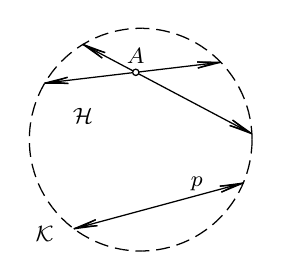
\begin{tikzpicture}
                    % \clip (0,0) rectangle (14.000000,10.000000);
                    {\footnotesize
                    
                    % Drawing circle k
                    \draw [line width=0.016cm] (4.414214,3.000000) arc (360:360:1.414214 and 1.414214) --(4.414214,3.000000) arc (0:3:1.414214 and 1.414214) -- (4.411478,3.087921);%
                    \draw [line width=0.016cm] (4.411478,3.087921) -- (4.410769,3.098651) arc (4:7:1.414214 and 1.414214) -- (4.403282,3.175502);%
                    \draw [line width=0.016cm] (4.389656,3.262404) -- (4.388230,3.269845) arc (11:14:1.414214 and 1.414214) -- (4.370654,3.348291);%
                    \draw [line width=0.016cm] (4.370654,3.348291) -- (4.366025,3.366025) arc (15:17:1.414214 and 1.414214) -- (4.346350,3.432830);%
                    \draw [line width=0.016cm] (4.316837,3.515695) -- (4.311236,3.529774) arc (22:24:1.414214 and 1.414214) -- (4.282229,3.596565);%
                    \draw [line width=0.016cm] (4.282229,3.596565) -- (4.281713,3.597672) arc (25:28:1.414214 and 1.414214) -- (4.242660,3.675126);%
                    \draw [line width=0.016cm] (4.198284,3.751076) -- (4.186059,3.770236) arc (33:35:1.414214 and 1.414214) -- (4.149272,3.824120);%
                    \draw [line width=0.016cm] (4.149272,3.824120) -- (4.144123,3.831254) arc (36:39:1.414214 and 1.414214) -- (4.095813,3.893976);%
                    \draw [line width=0.016cm] (4.038116,3.960373) -- (4.034290,3.964491) arc (43:46:1.414214 and 1.414214) -- (3.976401,4.023054);%
                    \draw [line width=0.016cm] (3.976401,4.023054) -- (3.964491,4.034290) arc (47:49:1.414214 and 1.414214) -- (3.910910,4.081778);%
                    \draw [line width=0.016cm] (3.841894,4.136316) -- (3.831254,4.144123) arc (54:57:1.414214 and 1.414214) -- (3.769621,4.186458);%
                    \draw [line width=0.016cm] (3.769621,4.186458) -- (3.749419,4.199321) arc (58:60:1.414214 and 1.414214) -- (3.694371,4.232010);%
                    \draw [line width=0.016cm] (3.616434,4.272796) -- (3.597673,4.281713) arc (65:67:1.414214 and 1.414214) -- (3.536112,4.308657);%
                    \draw [line width=0.016cm] (3.536112,4.308657) -- (3.529774,4.311236) arc (68:71:1.414214 and 1.414214) -- (3.453716,4.339456);%
                    \draw [line width=0.016cm] (3.369565,4.365072) -- (3.366025,4.366025) arc (75:78:1.414214 and 1.414214) -- (3.283984,4.385407);%
                    \draw [line width=0.016cm] (3.283984,4.385407) -- (3.269845,4.388230) arc (79:81:1.414214 and 1.414214) -- (3.197305,4.400382);%
                    \draw [line width=0.016cm] (3.109862,4.409940) -- (3.098651,4.410769) arc (86:89:1.414214 and 1.414214) -- (3.021994,4.414043);%
                    \draw [line width=0.016cm] (3.021994,4.414043) -- (3.000000,4.414214) arc (90:92:1.414214 and 1.414214) -- (2.934041,4.412675);%
                    \draw [line width=0.016cm] (2.846343,4.405841) -- (2.827651,4.403672) arc (97:99:1.414214 and 1.414214) -- (2.759239,4.393569);%
                    \draw [line width=0.016cm] (2.759239,4.393569) -- (2.754425,4.392729) arc (100:103:1.414214 and 1.414214) -- (2.673067,4.375905);%
                    \draw [line width=0.016cm] (2.588160,4.352918) -- (2.586524,4.352419) arc (107:110:1.414214 and 1.414214) -- (2.504847,4.324697);%
                    \draw [line width=0.016cm] (2.504847,4.324697) -- (2.493191,4.320282) arc (111:114:1.414214 and 1.414214) -- (2.423448,4.291351);%
                    \draw [line width=0.016cm] (2.344281,4.253009) -- (2.336067,4.248677) arc (118:121:1.414214 and 1.414214) -- (2.267650,4.209820);%
                    \draw [line width=0.016cm] (2.267650,4.209820) -- (2.250581,4.199321) arc (122:124:1.414214 and 1.414214) -- (2.193853,4.161950);%
                    \draw [line width=0.016cm] (2.123174,4.109584) -- (2.110007,4.099050) arc (129:131:1.414214 and 1.414214) -- (2.055888,4.052926);%
                    \draw [line width=0.016cm] (2.055888,4.052926) -- (2.053707,4.050966) arc (132:135:1.414214 and 1.414214) -- (1.992254,3.992194);%
                    \draw [line width=0.016cm] (1.932519,3.927623) -- (1.916650,3.909039) arc (140:142:1.414214 and 1.414214) -- (1.876914,3.859464);%
                    \draw [line width=0.016cm] (1.876914,3.859464) -- (1.870559,3.851095) arc (143:146:1.414214 and 1.414214) -- (1.825654,3.787980);%
                    \draw [line width=0.016cm] (1.778937,3.713447) -- (1.775255,3.707107) arc (150:153:1.414214 and 1.414214) -- (1.736945,3.636154);%
                    \draw [line width=0.016cm] (1.736945,3.636154) -- (1.728913,3.619951) arc (154:156:1.414214 and 1.414214) -- (1.699839,3.556399);%
                    \draw [line width=0.016cm] (1.667762,3.474492) -- (1.662835,3.460423) arc (161:163:1.414214 and 1.414214) -- (1.640840,3.390750);%
                    \draw [line width=0.016cm] (1.640840,3.390750) -- (1.640571,3.389810) arc (164:167:1.414214 and 1.414214) -- (1.619177,3.305496);%
                    \draw [line width=0.016cm] (1.602855,3.219059) -- (1.599549,3.196821) arc (172:174:1.414214 and 1.414214) -- (1.591939,3.131776);%
                    \draw [line width=0.016cm] (1.591939,3.131776) -- (1.591168,3.123257) arc (175:178:1.414214 and 1.414214) -- (1.586471,3.043982);%
                    \draw [line width=0.016cm] (1.586470,2.956019) -- (1.586648,2.950645) arc (182:185:1.414214 and 1.414214) -- (1.591939,2.868225);%
                    \draw [line width=0.016cm] (1.591939,2.868225) -- (1.593534,2.852175) arc (186:188:1.414214 and 1.414214) -- (1.602855,2.780942);%
                    \draw [line width=0.016cm] (1.619177,2.694505) -- (1.622033,2.681871) arc (193:196:1.414214 and 1.414214) -- (1.640840,2.609251);%
                    \draw [line width=0.016cm] (1.640840,2.609251) -- (1.647581,2.586524) arc (197:199:1.414214 and 1.414214) -- (1.667762,2.525508);%
                    \draw [line width=0.016cm] (1.699838,2.443602) -- (1.708052,2.424788) arc (204:206:1.414214 and 1.414214) -- (1.736944,2.363847);%
                    \draw [line width=0.016cm] (1.736944,2.363847) -- (1.739926,2.357961) arc (207:210:1.414214 and 1.414214) -- (1.778937,2.286554);%
                    \draw [line width=0.016cm] (1.825654,2.212021) -- (1.827564,2.209182) arc (214:217:1.414214 and 1.414214) -- (1.876914,2.140537);%
                    \draw [line width=0.016cm] (1.876914,2.140537) -- (1.885584,2.129323) arc (218:220:1.414214 and 1.414214) -- (1.932519,2.072377);%
                    \draw [line width=0.016cm] (1.992254,2.007807) -- (2.000000,2.000000) arc (225:228:1.414214 and 1.414214) -- (2.055887,1.947075);%
                    \draw [line width=0.016cm] (2.055887,1.947075) -- (2.072192,1.932680) arc (229:231:1.414214 and 1.414214) -- (2.123174,1.890417);%
                    \draw [line width=0.016cm] (2.193852,1.838051) -- (2.209182,1.827564) arc (236:238:1.414214 and 1.414214) -- (2.267649,1.790181);%
                    \draw [line width=0.016cm] (2.267649,1.790181) -- (2.271626,1.787783) arc (239:242:1.414214 and 1.414214) -- (2.344280,1.746991);%
                    \draw [line width=0.016cm] (2.423448,1.708649) -- (2.424787,1.708052) arc (246:249:1.414214 and 1.414214) -- (2.504846,1.675303);%
                    \draw [line width=0.016cm] (2.504846,1.675303) -- (2.516310,1.671074) arc (250:253:1.414214 and 1.414214) -- (2.588159,1.647082);%
                    \draw [line width=0.016cm] (2.673067,1.624095) -- (2.681871,1.622033) arc (257:260:1.414214 and 1.414214) -- (2.759239,1.606431);%
                    \draw [line width=0.016cm] (2.759239,1.606431) -- (2.778768,1.603198) arc (261:263:1.414214 and 1.414214) -- (2.846342,1.594159);%
                    \draw [line width=0.016cm] (2.934040,1.587325) -- (2.950644,1.586648) arc (268:270:1.414214 and 1.414214) -- (3.021993,1.585957);%
                    \draw [line width=0.016cm] (3.021993,1.585957) -- (3.024681,1.586002) arc (271:274:1.414214 and 1.414214) -- (3.109861,1.590060);%
                    \draw [line width=0.016cm] (3.197304,1.599617) -- (3.221231,1.603198) arc (279:281:1.414214 and 1.414214) -- (3.283983,1.614593);%
                    \draw [line width=0.016cm] (3.283983,1.614593) -- (3.294031,1.616690) arc (282:285:1.414214 and 1.414214) -- (3.369564,1.634928);%
                    \draw [line width=0.016cm] (3.453715,1.660544) -- (3.460423,1.662835) arc (289:292:1.414214 and 1.414214) -- (3.536111,1.691342);%
                    \draw [line width=0.016cm] (3.536111,1.691342) -- (3.552577,1.698209) arc (293:295:1.414214 and 1.414214) -- (3.616433,1.727204);%
                    \draw [line width=0.016cm] (3.694370,1.767989) -- (3.707106,1.775255) arc (300:302:1.414214 and 1.414214) -- (3.769620,1.813541);%
                    \draw [line width=0.016cm] (3.769620,1.813541) -- (3.770236,1.813941) arc (303:306:1.414214 and 1.414214) -- (3.841893,1.863683);%
                    \draw [line width=0.016cm] (3.910909,1.918222) -- (3.927807,1.932679) arc (311:313:1.414214 and 1.414214) -- (3.976401,1.976945);%
                    \draw [line width=0.016cm] (3.976401,1.976945) -- (3.982395,1.982700) arc (314:317:1.414214 and 1.414214) -- (4.038115,2.039626);%
                    \draw [line width=0.016cm] (4.095813,2.106023) -- (4.099050,2.110006) arc (321:324:1.414214 and 1.414214) -- (4.149271,2.175879);%
                    \draw [line width=0.016cm] (4.149271,2.175879) -- (4.158456,2.188840) arc (325:327:1.414214 and 1.414214) -- (4.198284,2.248923);%
                    \draw [line width=0.016cm] (4.242660,2.324873) -- (4.248676,2.336067) arc (332:335:1.414214 and 1.414214) -- (4.282228,2.403434);%
                    \draw [line width=0.016cm] (4.282228,2.403434) -- (4.291948,2.424787) arc (336:338:1.414214 and 1.414214) -- (4.316836,2.484304);%
                    \draw [line width=0.016cm] (4.346350,2.567169) -- (4.352419,2.586524) arc (343:345:1.414214 and 1.414214) -- (4.370654,2.651708);%
                    \draw [line width=0.016cm] (4.370654,2.651708) -- (4.372205,2.657870) arc (346:349:1.414214 and 1.414214) -- (4.389656,2.737595);%
                    \draw [line width=0.016cm] (4.403281,2.824497) -- (4.403672,2.827650) arc (353:356:1.414214 and 1.414214) -- (4.411478,2.912078);%
                    \draw [line width=0.016cm] (4.411478,2.912078) -- (4.412275,2.925985) arc (357:359:1.414214 and 1.414214) -- (4.414214,2.999999);%
                    
                    % Drawing segment G B
                    \draw [line width=0.016cm] (2.152000,1.868000) -- (4.302000,2.449000);%
                    
                    % Marking point p
                    \draw (3.531000,2.241000) node [anchor=south west] { $p$ };%
                    
                    % Drawing arrow G B 1.00
                    \draw [line width=0.016cm] (4.004651,2.409209) -- (4.302000,2.449000);%
                    \draw [line width=0.016cm] (4.004651,2.409209) -- (4.206289,2.423136);%
                    \draw [line width=0.016cm] (4.025081,2.333605) -- (4.302000,2.449000);%
                    \draw [line width=0.016cm] (4.025081,2.333605) -- (4.206289,2.423136);%
                    
                    % Drawing arrow B G 1.00
                    \draw [line width=0.016cm] (2.449349,1.907791) -- (2.152000,1.868000);%
                    \draw [line width=0.016cm] (2.449349,1.907791) -- (2.247711,1.893864);%
                    \draw [line width=0.016cm] (2.428919,1.983395) -- (2.152000,1.868000);%
                    \draw [line width=0.016cm] (2.428919,1.983395) -- (2.247711,1.893864);%
                    
                    % Marking point A by circle
                    \draw [line width=0.016cm] (2.937732,3.855090) circle (0.040000);%
                    \draw (2.937732,3.855090) node [anchor=south] { $A$ };%
                    
                    % Drawing segment E D
                    \draw [line width=0.016cm] (1.781000,3.718000) -- (2.898010,3.850383);%
                    \draw [line width=0.016cm] (2.977454,3.859798) -- (4.017000,3.983000);%
                    
                    % Drawing segment C F
                    \draw [line width=0.016cm] (2.267000,4.210000) -- (2.902377,3.873798);%
                    \draw [line width=0.016cm] (2.973088,3.836382) -- (4.412000,3.075000);%
                    
                    % Drawing arrow F C 1.00
                    \draw [line width=0.016cm] (2.511584,4.036280) -- (2.267000,4.210000);%
                    \draw [line width=0.016cm] (2.511584,4.036280) -- (2.354633,4.163630);%
                    \draw [line width=0.016cm] (2.548212,4.105502) -- (2.267000,4.210000);%
                    \draw [line width=0.016cm] (2.548212,4.105502) -- (2.354633,4.163630);%
                    
                    % Drawing arrow C F 1.00
                    \draw [line width=0.016cm] (4.167416,3.248720) -- (4.412000,3.075000);%
                    \draw [line width=0.016cm] (4.167416,3.248720) -- (4.324367,3.121370);%
                    \draw [line width=0.016cm] (4.130788,3.179498) -- (4.412000,3.075000);%
                    \draw [line width=0.016cm] (4.130788,3.179498) -- (4.324367,3.121370);%
                    
                    % Drawing arrow D E 1.00
                    \draw [line width=0.016cm] (2.080975,3.714120) -- (1.781000,3.718000);%
                    \draw [line width=0.016cm] (2.080975,3.714120) -- (1.879455,3.729668);%
                    \draw [line width=0.016cm] (2.071758,3.791891) -- (1.781000,3.718000);%
                    \draw [line width=0.016cm] (2.071758,3.791891) -- (1.879455,3.729668);%
                    
                    % Drawing arrow E D 1.00
                    \draw [line width=0.016cm] (3.717025,3.986880) -- (4.017000,3.983000);%
                    \draw [line width=0.016cm] (3.717025,3.986880) -- (3.918545,3.971332);%
                    \draw [line width=0.016cm] (3.726242,3.909109) -- (4.017000,3.983000);%
                    \draw [line width=0.016cm] (3.726242,3.909109) -- (3.918545,3.971332);%
                    
                    % Marking point \mathcal{K}
                    \draw (2.000000,2.000000) node [anchor=north east] { $\mathcal{K}$ };%

                    \draw (2.500000,3.500000) node [anchor=north east] { $\mathcal{H}$ };%

                    }
                \end{tikzpicture}     

            Očitno v tem modelu velja hiperbolični aksiom.

            Skladnost definiramo s pomočjo merjenja. Očitno dolžine daljic ne morejo biti evklidske. Enako velja za merjenje kotov, saj bi ob evklidskem merjenju kotov trikotniki imeli defekt enak 0.


        \subsection{Poincaréjev model na disku}

            Naj bo $\mathcal{K}=K(S,r)$ krožnica s središčem $S$ in polmerom $r$. 
            Hiperbolično ravnino $\mathcal{H}$ predstavlja notranjost krožnice $\mathcal{K}$, točke na krožnici $\mathcal{K}$ so idealne točke ravnine. 

            P-premice so dveh vrst: \begin{itemize}
                \item odprti premeri na $\mathcal{K}$,
                \item krožni loki v $\mathcal{H}$, ki so pravokotni na $\mathcal{K}$.
            \end{itemize}

                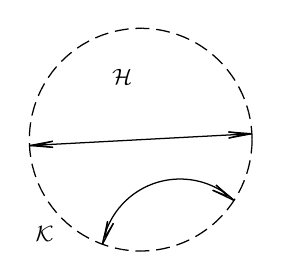
\begin{tikzpicture}
                    % \clip (0,0) rectangle (14.000000,10.000000);
                    {\footnotesize
                    
                    % Drawing circle k
                    \draw [line width=0.016cm] (4.414214,3.000000) arc (360:360:1.414214 and 1.414214) --(4.414214,3.000000) arc (0:3:1.414214 and 1.414214) -- (4.411478,3.087921);%
                    \draw [line width=0.016cm] (4.411478,3.087921) -- (4.410769,3.098651) arc (4:7:1.414214 and 1.414214) -- (4.403282,3.175502);%
                    \draw [line width=0.016cm] (4.389656,3.262404) -- (4.388230,3.269845) arc (11:14:1.414214 and 1.414214) -- (4.370654,3.348291);%
                    \draw [line width=0.016cm] (4.370654,3.348291) -- (4.366025,3.366025) arc (15:17:1.414214 and 1.414214) -- (4.346350,3.432830);%
                    \draw [line width=0.016cm] (4.316837,3.515695) -- (4.311236,3.529774) arc (22:24:1.414214 and 1.414214) -- (4.282229,3.596565);%
                    \draw [line width=0.016cm] (4.282229,3.596565) -- (4.281713,3.597672) arc (25:28:1.414214 and 1.414214) -- (4.242660,3.675126);%
                    \draw [line width=0.016cm] (4.198284,3.751076) -- (4.186059,3.770236) arc (33:35:1.414214 and 1.414214) -- (4.149272,3.824120);%
                    \draw [line width=0.016cm] (4.149272,3.824120) -- (4.144123,3.831254) arc (36:39:1.414214 and 1.414214) -- (4.095813,3.893976);%
                    \draw [line width=0.016cm] (4.038116,3.960373) -- (4.034290,3.964491) arc (43:46:1.414214 and 1.414214) -- (3.976401,4.023054);%
                    \draw [line width=0.016cm] (3.976401,4.023054) -- (3.964491,4.034290) arc (47:49:1.414214 and 1.414214) -- (3.910910,4.081778);%
                    \draw [line width=0.016cm] (3.841894,4.136316) -- (3.831254,4.144123) arc (54:57:1.414214 and 1.414214) -- (3.769621,4.186458);%
                    \draw [line width=0.016cm] (3.769621,4.186458) -- (3.749419,4.199321) arc (58:60:1.414214 and 1.414214) -- (3.694371,4.232010);%
                    \draw [line width=0.016cm] (3.616434,4.272796) -- (3.597673,4.281713) arc (65:67:1.414214 and 1.414214) -- (3.536112,4.308657);%
                    \draw [line width=0.016cm] (3.536112,4.308657) -- (3.529774,4.311236) arc (68:71:1.414214 and 1.414214) -- (3.453716,4.339456);%
                    \draw [line width=0.016cm] (3.369565,4.365072) -- (3.366025,4.366025) arc (75:78:1.414214 and 1.414214) -- (3.283984,4.385407);%
                    \draw [line width=0.016cm] (3.283984,4.385407) -- (3.269845,4.388230) arc (79:81:1.414214 and 1.414214) -- (3.197305,4.400382);%
                    \draw [line width=0.016cm] (3.109862,4.409940) -- (3.098651,4.410769) arc (86:89:1.414214 and 1.414214) -- (3.021994,4.414043);%
                    \draw [line width=0.016cm] (3.021994,4.414043) -- (3.000000,4.414214) arc (90:92:1.414214 and 1.414214) -- (2.934041,4.412675);%
                    \draw [line width=0.016cm] (2.846343,4.405841) -- (2.827651,4.403672) arc (97:99:1.414214 and 1.414214) -- (2.759239,4.393569);%
                    \draw [line width=0.016cm] (2.759239,4.393569) -- (2.754425,4.392729) arc (100:103:1.414214 and 1.414214) -- (2.673067,4.375905);%
                    \draw [line width=0.016cm] (2.588160,4.352918) -- (2.586524,4.352419) arc (107:110:1.414214 and 1.414214) -- (2.504847,4.324697);%
                    \draw [line width=0.016cm] (2.504847,4.324697) -- (2.493191,4.320282) arc (111:114:1.414214 and 1.414214) -- (2.423448,4.291351);%
                    \draw [line width=0.016cm] (2.344281,4.253009) -- (2.336067,4.248677) arc (118:121:1.414214 and 1.414214) -- (2.267650,4.209820);%
                    \draw [line width=0.016cm] (2.267650,4.209820) -- (2.250581,4.199321) arc (122:124:1.414214 and 1.414214) -- (2.193853,4.161950);%
                    \draw [line width=0.016cm] (2.123174,4.109584) -- (2.110007,4.099050) arc (129:131:1.414214 and 1.414214) -- (2.055888,4.052926);%
                    \draw [line width=0.016cm] (2.055888,4.052926) -- (2.053707,4.050966) arc (132:135:1.414214 and 1.414214) -- (1.992254,3.992194);%
                    \draw [line width=0.016cm] (1.932519,3.927623) -- (1.916650,3.909039) arc (140:142:1.414214 and 1.414214) -- (1.876914,3.859464);%
                    \draw [line width=0.016cm] (1.876914,3.859464) -- (1.870559,3.851095) arc (143:146:1.414214 and 1.414214) -- (1.825654,3.787980);%
                    \draw [line width=0.016cm] (1.778937,3.713447) -- (1.775255,3.707107) arc (150:153:1.414214 and 1.414214) -- (1.736945,3.636154);%
                    \draw [line width=0.016cm] (1.736945,3.636154) -- (1.728913,3.619951) arc (154:156:1.414214 and 1.414214) -- (1.699839,3.556399);%
                    \draw [line width=0.016cm] (1.667762,3.474492) -- (1.662835,3.460423) arc (161:163:1.414214 and 1.414214) -- (1.640840,3.390750);%
                    \draw [line width=0.016cm] (1.640840,3.390750) -- (1.640571,3.389810) arc (164:167:1.414214 and 1.414214) -- (1.619177,3.305496);%
                    \draw [line width=0.016cm] (1.602855,3.219059) -- (1.599549,3.196821) arc (172:174:1.414214 and 1.414214) -- (1.591939,3.131776);%
                    \draw [line width=0.016cm] (1.591939,3.131776) -- (1.591168,3.123257) arc (175:178:1.414214 and 1.414214) -- (1.586471,3.043982);%
                    \draw [line width=0.016cm] (1.586470,2.956019) -- (1.586648,2.950645) arc (182:185:1.414214 and 1.414214) -- (1.591939,2.868225);%
                    \draw [line width=0.016cm] (1.591939,2.868225) -- (1.593534,2.852175) arc (186:188:1.414214 and 1.414214) -- (1.602855,2.780942);%
                    \draw [line width=0.016cm] (1.619177,2.694505) -- (1.622033,2.681871) arc (193:196:1.414214 and 1.414214) -- (1.640840,2.609251);%
                    \draw [line width=0.016cm] (1.640840,2.609251) -- (1.647581,2.586524) arc (197:199:1.414214 and 1.414214) -- (1.667762,2.525508);%
                    \draw [line width=0.016cm] (1.699838,2.443602) -- (1.708052,2.424788) arc (204:206:1.414214 and 1.414214) -- (1.736944,2.363847);%
                    \draw [line width=0.016cm] (1.736944,2.363847) -- (1.739926,2.357961) arc (207:210:1.414214 and 1.414214) -- (1.778937,2.286554);%
                    \draw [line width=0.016cm] (1.825654,2.212021) -- (1.827564,2.209182) arc (214:217:1.414214 and 1.414214) -- (1.876914,2.140537);%
                    \draw [line width=0.016cm] (1.876914,2.140537) -- (1.885584,2.129323) arc (218:220:1.414214 and 1.414214) -- (1.932519,2.072377);%
                    \draw [line width=0.016cm] (1.992254,2.007807) -- (2.000000,2.000000) arc (225:228:1.414214 and 1.414214) -- (2.055887,1.947075);%
                    \draw [line width=0.016cm] (2.055887,1.947075) -- (2.072192,1.932680) arc (229:231:1.414214 and 1.414214) -- (2.123174,1.890417);%
                    \draw [line width=0.016cm] (2.193852,1.838051) -- (2.209182,1.827564) arc (236:238:1.414214 and 1.414214) -- (2.267649,1.790181);%
                    \draw [line width=0.016cm] (2.267649,1.790181) -- (2.271626,1.787783) arc (239:242:1.414214 and 1.414214) -- (2.344280,1.746991);%
                    \draw [line width=0.016cm] (2.423448,1.708649) -- (2.424787,1.708052) arc (246:249:1.414214 and 1.414214) -- (2.504846,1.675303);%
                    \draw [line width=0.016cm] (2.504846,1.675303) -- (2.516310,1.671074) arc (250:253:1.414214 and 1.414214) -- (2.588159,1.647082);%
                    \draw [line width=0.016cm] (2.673067,1.624095) -- (2.681871,1.622033) arc (257:260:1.414214 and 1.414214) -- (2.759239,1.606431);%
                    \draw [line width=0.016cm] (2.759239,1.606431) -- (2.778768,1.603198) arc (261:263:1.414214 and 1.414214) -- (2.846342,1.594159);%
                    \draw [line width=0.016cm] (2.934040,1.587325) -- (2.950644,1.586648) arc (268:270:1.414214 and 1.414214) -- (3.021993,1.585957);%
                    \draw [line width=0.016cm] (3.021993,1.585957) -- (3.024681,1.586002) arc (271:274:1.414214 and 1.414214) -- (3.109861,1.590060);%
                    \draw [line width=0.016cm] (3.197304,1.599617) -- (3.221231,1.603198) arc (279:281:1.414214 and 1.414214) -- (3.283983,1.614593);%
                    \draw [line width=0.016cm] (3.283983,1.614593) -- (3.294031,1.616690) arc (282:285:1.414214 and 1.414214) -- (3.369564,1.634928);%
                    \draw [line width=0.016cm] (3.453715,1.660544) -- (3.460423,1.662835) arc (289:292:1.414214 and 1.414214) -- (3.536111,1.691342);%
                    \draw [line width=0.016cm] (3.536111,1.691342) -- (3.552577,1.698209) arc (293:295:1.414214 and 1.414214) -- (3.616433,1.727204);%
                    \draw [line width=0.016cm] (3.694370,1.767989) -- (3.707106,1.775255) arc (300:302:1.414214 and 1.414214) -- (3.769620,1.813541);%
                    \draw [line width=0.016cm] (3.769620,1.813541) -- (3.770236,1.813941) arc (303:306:1.414214 and 1.414214) -- (3.841893,1.863683);%
                    \draw [line width=0.016cm] (3.910909,1.918222) -- (3.927807,1.932679) arc (311:313:1.414214 and 1.414214) -- (3.976401,1.976945);%
                    \draw [line width=0.016cm] (3.976401,1.976945) -- (3.982395,1.982700) arc (314:317:1.414214 and 1.414214) -- (4.038115,2.039626);%
                    \draw [line width=0.016cm] (4.095813,2.106023) -- (4.099050,2.110006) arc (321:324:1.414214 and 1.414214) -- (4.149271,2.175879);%
                    \draw [line width=0.016cm] (4.149271,2.175879) -- (4.158456,2.188840) arc (325:327:1.414214 and 1.414214) -- (4.198284,2.248923);%
                    \draw [line width=0.016cm] (4.242660,2.324873) -- (4.248676,2.336067) arc (332:335:1.414214 and 1.414214) -- (4.282228,2.403434);%
                    \draw [line width=0.016cm] (4.282228,2.403434) -- (4.291948,2.424787) arc (336:338:1.414214 and 1.414214) -- (4.316836,2.484304);%
                    \draw [line width=0.016cm] (4.346350,2.567169) -- (4.352419,2.586524) arc (343:345:1.414214 and 1.414214) -- (4.370654,2.651708);%
                    \draw [line width=0.016cm] (4.370654,2.651708) -- (4.372205,2.657870) arc (346:349:1.414214 and 1.414214) -- (4.389656,2.737595);%
                    \draw [line width=0.016cm] (4.403281,2.824497) -- (4.403672,2.827650) arc (353:356:1.414214 and 1.414214) -- (4.411478,2.912078);%
                    \draw [line width=0.016cm] (4.411478,2.912078) -- (4.412275,2.925985) arc (357:359:1.414214 and 1.414214) -- (4.414214,2.999999);%
                    
                    % Drawing segment I J
                    \draw [line width=0.016cm] (4.412223,3.075012) -- (1.587777,2.924988);%
                    
                    % Drawing arrow I J 1.00
                    \draw [line width=0.016cm] (1.886869,2.901662) -- (1.587777,2.924988);%
                    \draw [line width=0.016cm] (1.886869,2.901662) -- (1.686782,2.930247);%
                    \draw [line width=0.016cm] (1.882715,2.979867) -- (1.587777,2.924988);%
                    \draw [line width=0.016cm] (1.882715,2.979867) -- (1.686782,2.930247);%
                    
                    % Drawing arrow J I 1.00
                    \draw [line width=0.016cm] (4.113131,3.098338) -- (4.412223,3.075012);%
                    \draw [line width=0.016cm] (4.113131,3.098338) -- (4.313218,3.069753);%
                    \draw [line width=0.016cm] (4.117285,3.020133) -- (4.412223,3.075012);%
                    \draw [line width=0.016cm] (4.117285,3.020133) -- (4.313218,3.069753);%
                    
                    % Drawing arc P N 123.37
                    \draw [line width=0.016cm] (4.185165,2.228388) -- (4.181998,2.231354) arc (47:170:1.000000 and 1.000000) -- (2.514835,1.671612);%
                    
                    % Marking point \mathcal{K}
                    \draw (2.000000,2.000000) node [anchor=north east] { $\mathcal{K}$ };%

                    \draw (3.000000,4.000000) node [anchor=north east] { $\mathcal{H}$ };%

                    
                    % Drawing arrow S M 1.00
                    \draw [line width=0.016cm] (2.653655,1.937561) -- (2.514835,1.671612);%
                    \draw [line width=0.016cm] (2.653655,1.937561) -- (2.548848,1.764739);%
                    \draw [line width=0.016cm] (2.580092,1.964428) -- (2.514835,1.671612);%
                    \draw [line width=0.016cm] (2.580092,1.964428) -- (2.548848,1.764739);%
                    
                    % Drawing arrow S N 1.00
                    \draw [line width=0.016cm] (3.957269,2.423487) -- (4.185165,2.228388);%
                    \draw [line width=0.016cm] (3.957269,2.423487) -- (4.102078,2.282483);%
                    \draw [line width=0.016cm] (3.914539,2.357856) -- (4.185165,2.228388);%
                    \draw [line width=0.016cm] (3.914539,2.357856) -- (4.102078,2.282483);%
                    }
                \end{tikzpicture}
                
            P-trikotnik sestoji iz P-daljic, ki so deli P-premic.

            Kote lahko merimo evklidsko kot kote med krivuljami in dobimo trikotnike s pozitivnimi defekti.

            Tako kot v prejšnjem primeru je jasno, kaj pomeni 'leži na' in 'leži med'.

            Skladnost daljic definiramo preko merjenja dolžin: 
                hiperbolična dolžina daljice $AB$: $d(A, B)=\left|\log (AB, \Omega\Sigma)\right|$, kjer je $(AB, \Omega\Sigma)=\frac{|A\Omega|\cdot|B\Sigma|}{|A\Sigma|\cdot|B\Omega|}$
            
                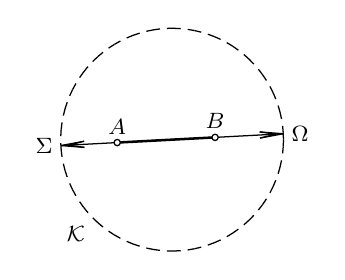
\begin{tikzpicture}
                    % \clip (0,0) rectangle (14.000000,10.000000);
                    {\footnotesize
                    
                    % Drawing circle k
                    \draw [line width=0.016cm] (4.414214,3.000000) arc (360:360:1.414214 and 1.414214) --(4.414214,3.000000) arc (0:3:1.414214 and 1.414214) -- (4.411478,3.087921);%
                    \draw [line width=0.016cm] (4.411478,3.087921) -- (4.410769,3.098651) arc (4:7:1.414214 and 1.414214) -- (4.403282,3.175502);%
                    \draw [line width=0.016cm] (4.389656,3.262404) -- (4.388230,3.269845) arc (11:14:1.414214 and 1.414214) -- (4.370654,3.348291);%
                    \draw [line width=0.016cm] (4.370654,3.348291) -- (4.366025,3.366025) arc (15:17:1.414214 and 1.414214) -- (4.346350,3.432830);%
                    \draw [line width=0.016cm] (4.316837,3.515695) -- (4.311236,3.529774) arc (22:24:1.414214 and 1.414214) -- (4.282229,3.596565);%
                    \draw [line width=0.016cm] (4.282229,3.596565) -- (4.281713,3.597672) arc (25:28:1.414214 and 1.414214) -- (4.242660,3.675126);%
                    \draw [line width=0.016cm] (4.198284,3.751076) -- (4.186059,3.770236) arc (33:35:1.414214 and 1.414214) -- (4.149272,3.824120);%
                    \draw [line width=0.016cm] (4.149272,3.824120) -- (4.144123,3.831254) arc (36:39:1.414214 and 1.414214) -- (4.095813,3.893976);%
                    \draw [line width=0.016cm] (4.038116,3.960373) -- (4.034290,3.964491) arc (43:46:1.414214 and 1.414214) -- (3.976401,4.023054);%
                    \draw [line width=0.016cm] (3.976401,4.023054) -- (3.964491,4.034290) arc (47:49:1.414214 and 1.414214) -- (3.910910,4.081778);%
                    \draw [line width=0.016cm] (3.841894,4.136316) -- (3.831254,4.144123) arc (54:57:1.414214 and 1.414214) -- (3.769621,4.186458);%
                    \draw [line width=0.016cm] (3.769621,4.186458) -- (3.749419,4.199321) arc (58:60:1.414214 and 1.414214) -- (3.694371,4.232010);%
                    \draw [line width=0.016cm] (3.616434,4.272796) -- (3.597673,4.281713) arc (65:67:1.414214 and 1.414214) -- (3.536112,4.308657);%
                    \draw [line width=0.016cm] (3.536112,4.308657) -- (3.529774,4.311236) arc (68:71:1.414214 and 1.414214) -- (3.453716,4.339456);%
                    \draw [line width=0.016cm] (3.369565,4.365072) -- (3.366025,4.366025) arc (75:78:1.414214 and 1.414214) -- (3.283984,4.385407);%
                    \draw [line width=0.016cm] (3.283984,4.385407) -- (3.269845,4.388230) arc (79:81:1.414214 and 1.414214) -- (3.197305,4.400382);%
                    \draw [line width=0.016cm] (3.109862,4.409940) -- (3.098651,4.410769) arc (86:89:1.414214 and 1.414214) -- (3.021994,4.414043);%
                    \draw [line width=0.016cm] (3.021994,4.414043) -- (3.000000,4.414214) arc (90:92:1.414214 and 1.414214) -- (2.934041,4.412675);%
                    \draw [line width=0.016cm] (2.846343,4.405841) -- (2.827651,4.403672) arc (97:99:1.414214 and 1.414214) -- (2.759239,4.393569);%
                    \draw [line width=0.016cm] (2.759239,4.393569) -- (2.754425,4.392729) arc (100:103:1.414214 and 1.414214) -- (2.673067,4.375905);%
                    \draw [line width=0.016cm] (2.588160,4.352918) -- (2.586524,4.352419) arc (107:110:1.414214 and 1.414214) -- (2.504847,4.324697);%
                    \draw [line width=0.016cm] (2.504847,4.324697) -- (2.493191,4.320282) arc (111:114:1.414214 and 1.414214) -- (2.423448,4.291351);%
                    \draw [line width=0.016cm] (2.344281,4.253009) -- (2.336067,4.248677) arc (118:121:1.414214 and 1.414214) -- (2.267650,4.209820);%
                    \draw [line width=0.016cm] (2.267650,4.209820) -- (2.250581,4.199321) arc (122:124:1.414214 and 1.414214) -- (2.193853,4.161950);%
                    \draw [line width=0.016cm] (2.123174,4.109584) -- (2.110007,4.099050) arc (129:131:1.414214 and 1.414214) -- (2.055888,4.052926);%
                    \draw [line width=0.016cm] (2.055888,4.052926) -- (2.053707,4.050966) arc (132:135:1.414214 and 1.414214) -- (1.992254,3.992194);%
                    \draw [line width=0.016cm] (1.932519,3.927623) -- (1.916650,3.909039) arc (140:142:1.414214 and 1.414214) -- (1.876914,3.859464);%
                    \draw [line width=0.016cm] (1.876914,3.859464) -- (1.870559,3.851095) arc (143:146:1.414214 and 1.414214) -- (1.825654,3.787980);%
                    \draw [line width=0.016cm] (1.778937,3.713447) -- (1.775255,3.707107) arc (150:153:1.414214 and 1.414214) -- (1.736945,3.636154);%
                    \draw [line width=0.016cm] (1.736945,3.636154) -- (1.728913,3.619951) arc (154:156:1.414214 and 1.414214) -- (1.699839,3.556399);%
                    \draw [line width=0.016cm] (1.667762,3.474492) -- (1.662835,3.460423) arc (161:163:1.414214 and 1.414214) -- (1.640840,3.390750);%
                    \draw [line width=0.016cm] (1.640840,3.390750) -- (1.640571,3.389810) arc (164:167:1.414214 and 1.414214) -- (1.619177,3.305496);%
                    \draw [line width=0.016cm] (1.602855,3.219059) -- (1.599549,3.196821) arc (172:174:1.414214 and 1.414214) -- (1.591939,3.131776);%
                    \draw [line width=0.016cm] (1.591939,3.131776) -- (1.591168,3.123257) arc (175:178:1.414214 and 1.414214) -- (1.586471,3.043982);%
                    \draw [line width=0.016cm] (1.586470,2.956019) -- (1.586648,2.950645) arc (182:185:1.414214 and 1.414214) -- (1.591939,2.868225);%
                    \draw [line width=0.016cm] (1.591939,2.868225) -- (1.593534,2.852175) arc (186:188:1.414214 and 1.414214) -- (1.602855,2.780942);%
                    \draw [line width=0.016cm] (1.619177,2.694505) -- (1.622033,2.681871) arc (193:196:1.414214 and 1.414214) -- (1.640840,2.609251);%
                    \draw [line width=0.016cm] (1.640840,2.609251) -- (1.647581,2.586524) arc (197:199:1.414214 and 1.414214) -- (1.667762,2.525508);%
                    \draw [line width=0.016cm] (1.699838,2.443602) -- (1.708052,2.424788) arc (204:206:1.414214 and 1.414214) -- (1.736944,2.363847);%
                    \draw [line width=0.016cm] (1.736944,2.363847) -- (1.739926,2.357961) arc (207:210:1.414214 and 1.414214) -- (1.778937,2.286554);%
                    \draw [line width=0.016cm] (1.825654,2.212021) -- (1.827564,2.209182) arc (214:217:1.414214 and 1.414214) -- (1.876914,2.140537);%
                    \draw [line width=0.016cm] (1.876914,2.140537) -- (1.885584,2.129323) arc (218:220:1.414214 and 1.414214) -- (1.932519,2.072377);%
                    \draw [line width=0.016cm] (1.992254,2.007807) -- (2.000000,2.000000) arc (225:228:1.414214 and 1.414214) -- (2.055887,1.947075);%
                    \draw [line width=0.016cm] (2.055887,1.947075) -- (2.072192,1.932680) arc (229:231:1.414214 and 1.414214) -- (2.123174,1.890417);%
                    \draw [line width=0.016cm] (2.193852,1.838051) -- (2.209182,1.827564) arc (236:238:1.414214 and 1.414214) -- (2.267649,1.790181);%
                    \draw [line width=0.016cm] (2.267649,1.790181) -- (2.271626,1.787783) arc (239:242:1.414214 and 1.414214) -- (2.344280,1.746991);%
                    \draw [line width=0.016cm] (2.423448,1.708649) -- (2.424787,1.708052) arc (246:249:1.414214 and 1.414214) -- (2.504846,1.675303);%
                    \draw [line width=0.016cm] (2.504846,1.675303) -- (2.516310,1.671074) arc (250:253:1.414214 and 1.414214) -- (2.588159,1.647082);%
                    \draw [line width=0.016cm] (2.673067,1.624095) -- (2.681871,1.622033) arc (257:260:1.414214 and 1.414214) -- (2.759239,1.606431);%
                    \draw [line width=0.016cm] (2.759239,1.606431) -- (2.778768,1.603198) arc (261:263:1.414214 and 1.414214) -- (2.846342,1.594159);%
                    \draw [line width=0.016cm] (2.934040,1.587325) -- (2.950644,1.586648) arc (268:270:1.414214 and 1.414214) -- (3.021993,1.585957);%
                    \draw [line width=0.016cm] (3.021993,1.585957) -- (3.024681,1.586002) arc (271:274:1.414214 and 1.414214) -- (3.109861,1.590060);%
                    \draw [line width=0.016cm] (3.197304,1.599617) -- (3.221231,1.603198) arc (279:281:1.414214 and 1.414214) -- (3.283983,1.614593);%
                    \draw [line width=0.016cm] (3.283983,1.614593) -- (3.294031,1.616690) arc (282:285:1.414214 and 1.414214) -- (3.369564,1.634928);%
                    \draw [line width=0.016cm] (3.453715,1.660544) -- (3.460423,1.662835) arc (289:292:1.414214 and 1.414214) -- (3.536111,1.691342);%
                    \draw [line width=0.016cm] (3.536111,1.691342) -- (3.552577,1.698209) arc (293:295:1.414214 and 1.414214) -- (3.616433,1.727204);%
                    \draw [line width=0.016cm] (3.694370,1.767989) -- (3.707106,1.775255) arc (300:302:1.414214 and 1.414214) -- (3.769620,1.813541);%
                    \draw [line width=0.016cm] (3.769620,1.813541) -- (3.770236,1.813941) arc (303:306:1.414214 and 1.414214) -- (3.841893,1.863683);%
                    \draw [line width=0.016cm] (3.910909,1.918222) -- (3.927807,1.932679) arc (311:313:1.414214 and 1.414214) -- (3.976401,1.976945);%
                    \draw [line width=0.016cm] (3.976401,1.976945) -- (3.982395,1.982700) arc (314:317:1.414214 and 1.414214) -- (4.038115,2.039626);%
                    \draw [line width=0.016cm] (4.095813,2.106023) -- (4.099050,2.110006) arc (321:324:1.414214 and 1.414214) -- (4.149271,2.175879);%
                    \draw [line width=0.016cm] (4.149271,2.175879) -- (4.158456,2.188840) arc (325:327:1.414214 and 1.414214) -- (4.198284,2.248923);%
                    \draw [line width=0.016cm] (4.242660,2.324873) -- (4.248676,2.336067) arc (332:335:1.414214 and 1.414214) -- (4.282228,2.403434);%
                    \draw [line width=0.016cm] (4.282228,2.403434) -- (4.291948,2.424787) arc (336:338:1.414214 and 1.414214) -- (4.316836,2.484304);%
                    \draw [line width=0.016cm] (4.346350,2.567169) -- (4.352419,2.586524) arc (343:345:1.414214 and 1.414214) -- (4.370654,2.651708);%
                    \draw [line width=0.016cm] (4.370654,2.651708) -- (4.372205,2.657870) arc (346:349:1.414214 and 1.414214) -- (4.389656,2.737595);%
                    \draw [line width=0.016cm] (4.403281,2.824497) -- (4.403672,2.827650) arc (353:356:1.414214 and 1.414214) -- (4.411478,2.912078);%
                    \draw [line width=0.016cm] (4.411478,2.912078) -- (4.412275,2.925985) arc (357:359:1.414214 and 1.414214) -- (4.414214,2.999999);%
                    
                    % Drawing segment I J
                    \draw [line width=0.016cm] (4.412223,3.075012) -- (3.585944,3.031123);%
                    \draw [line width=0.016cm] (3.506056,3.026880) -- (2.342945,2.965100);%
                    \draw [line width=0.016cm] (2.263057,2.960856) -- (1.587777,2.924988);%
                    
                    % Drawing arrow I J 1.00
                    \draw [line width=0.016cm] (1.886869,2.901662) -- (1.587777,2.924988);%
                    \draw [line width=0.016cm] (1.886869,2.901662) -- (1.686782,2.930247);%
                    \draw [line width=0.016cm] (1.882715,2.979867) -- (1.587777,2.924988);%
                    \draw [line width=0.016cm] (1.882715,2.979867) -- (1.686782,2.930247);%
                    
                    % Drawing arrow J I 1.00
                    \draw [line width=0.016cm] (4.113131,3.098338) -- (4.412223,3.075012);%
                    \draw [line width=0.016cm] (4.113131,3.098338) -- (4.313218,3.069753);%
                    \draw [line width=0.016cm] (4.117285,3.020133) -- (4.412223,3.075012);%
                    \draw [line width=0.016cm] (4.117285,3.020133) -- (4.313218,3.069753);%
                    
                    % Marking point A by circle
                    \draw [line width=0.016cm] (2.303000,2.963000) circle (0.040000);%
                    \draw (2.303000,2.963000) node [anchor=south] { $A$ };%
                    
                    % Marking point B by circle
                    \draw [line width=0.016cm] (3.546000,3.029000) circle (0.040000);%
                    \draw (3.546000,3.029000) node [anchor=south] { $B$ };%
                    
                    % Marking point \Sigma
                    \draw (1.588000,2.925000) node [anchor=east] { $\Sigma$ };%
                    
                    % Marking point \Omega
                    \draw (4.412000,3.075000) node [anchor=west] { $\Omega$ };%
                    
                    % Marking point \mathcal{K}
                    \draw (2.000000,2.000000) node [anchor=north east] { $\mathcal{K}$ };%
                    
                    % Drawing segment A B
                    \draw [line width=0.032cm] (2.342944,2.965121) -- (3.506056,3.026879);%
                    }
                \end{tikzpicture}
                    
            Dolžina $d(A, B)$ je neodvisna od vrstnega reda idealnih točk $\Omega$ in $\Sigma$, zato velja: $(AB, \Omega\Sigma)=\frac{1}{(AB, \Sigma\Omega)}$


        \subsection{Poincaréjev model na zgornji polravnini}

            $\mathcal{H}=\{(x,y); y>0\}$

            Premice so: (1) poltraki pravokotni na x-os, in (2) polkrožnice s središčem na x-osi.
            
                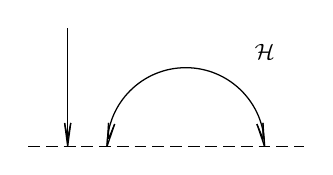
\begin{tikzpicture}
                    % \clip (0,0) rectangle (14.000000,10.000000);
                    {\footnotesize
                    
                    % Drawing line A B
                    \draw [line width=0.016cm] (1.500000,1.500000) -- (1.650000,1.500000);%
                    \draw [line width=0.016cm] (1.725000,1.500000) -- (1.875000,1.500000);%
                    \draw [line width=0.016cm] (1.950000,1.500000) -- (2.100000,1.500000);%
                    \draw [line width=0.016cm] (2.175000,1.500000) -- (2.325000,1.500000);%
                    \draw [line width=0.016cm] (2.400000,1.500000) -- (2.550000,1.500000);%
                    \draw [line width=0.016cm] (2.625000,1.500000) -- (2.775000,1.500000);%
                    \draw [line width=0.016cm] (2.850000,1.500000) -- (3.000000,1.500000);%
                    \draw [line width=0.016cm] (3.075000,1.500000) -- (3.225000,1.500000);%
                    \draw [line width=0.016cm] (3.300000,1.500000) -- (3.450000,1.500000);%
                    \draw [line width=0.016cm] (3.525000,1.500000) -- (3.675000,1.500000);%
                    \draw [line width=0.016cm] (3.750000,1.500000) -- (3.900000,1.500000);%
                    \draw [line width=0.016cm] (3.975000,1.500000) -- (4.125000,1.500000);%
                    \draw [line width=0.016cm] (4.200000,1.500000) -- (4.350000,1.500000);%
                    \draw [line width=0.016cm] (4.425000,1.500000) -- (4.575000,1.500000);%
                    \draw [line width=0.016cm] (4.650000,1.500000) -- (4.800000,1.500000);%
                    \draw [line width=0.016cm] (4.875000,1.500000) -- (5.000000,1.500000);%
                    
                    % Drawing segment A C
                    \draw [line width=0.016cm] (2.000000,1.500000) -- (2.000000,3.000000);%
                    
                    % Drawing arrow C A 1.00
                    \draw [line width=0.016cm] (2.039158,1.797433) -- (2.000000,1.500000);%
                    \draw [line width=0.016cm] (2.039158,1.797433) -- (2.000000,1.599144);%
                    \draw [line width=0.016cm] (1.960842,1.797433) -- (2.000000,1.500000);%
                    \draw [line width=0.016cm] (1.960842,1.797433) -- (2.000000,1.599144);%
                    
                    % Drawing circle E D
                    \draw [line width=0.016cm] (4.500000,1.500000) arc (360:360:1.000000 and 1.000000) --(4.500000,1.500000) arc (0:180:1.000000 and 1.000000);%
                    
                    % Drawing arrow F D 1.00
                    \draw [line width=0.016cm] (2.596729,1.783978) -- (2.500000,1.500000);%
                    \draw [line width=0.016cm] (2.596729,1.783978) -- (2.519444,1.597219);%
                    \draw [line width=0.016cm] (2.519934,1.799337) -- (2.500000,1.500000);%
                    \draw [line width=0.016cm] (2.519934,1.799337) -- (2.519444,1.597219);%
                    
                    % Drawing arrow G H 1.00
                    \draw [line width=0.016cm] (4.480066,1.799337) -- (4.500000,1.500000);%
                    \draw [line width=0.016cm] (4.480066,1.799337) -- (4.480556,1.597219);%
                    \draw [line width=0.016cm] (4.403271,1.783978) -- (4.500000,1.500000);%
                    \draw [line width=0.016cm] (4.403271,1.783978) -- (4.480556,1.597219);%
                    
                    % Marking point \mathcal{H}
                    \draw (4.500000,2.500000) node [anchor=south] { $\mathcal{H}$ };%
                    }
                \end{tikzpicture}
                
            Relacije 'leži na', 'leži med' so definirane podobno kot v prejšnjem modelu.
            
            Skladnost definiramo z merjenjem -- kote merimo evklidsko kot kote med krivuljami, razdalje bolj komplicirano.
            
            Ta model lahko povežemo s prejšnjim preko kompleksne preslikave ($\varphi(z)=\frac{z-i}{z+1}$), ki ohranja kote in preko te preslikave lahko prenesmo pojem razdalje oziroma dolžine daljice.


        \subsection{Imaginarna sfera v prostoru Minkowskega}

            $\RR^3$ s koordinatami $(x,y,t)$ opremimo z metriko Minkowskega, ki je porojena z normo $i:~\left\lVert (x,y,t)\right\rVert^2=x^2+y^2-t^2$.
           
            Množica točk z normo $i$ ustreza enačbi $x^2+y^2-t^2=-1$~$\to$~$t^2=x^2+y^2+1$.
           
            Vzamemo $\mathcal{H}=\{(x,y,t)\in\RR^3 | x^2+y^2-t^2=-1, t\geq 1\}$. To je zgornji del hiperboloida. Premice so presečišča $\mathcal{H}$ z ravninami skozi izhodišče in so hiperbole.
           
            \begin{figure}[H]

                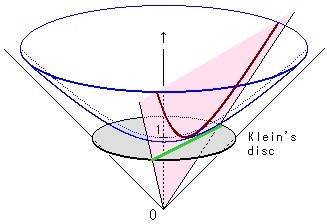
\includegraphics[scale=0.5]{Skice/ktop61.jpeg}
                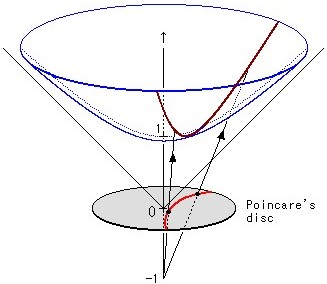
\includegraphics[scale=0.5]{Skice/ktop62.jpeg}
            \end{figure}
            
            Disk s središčem v $(0,0,1)$ in polmerom $1$, ki je tangenten na $\mathcal{H}$, si lahko predstavljamo kot Beltrami-Kleinov model hiperbolične geometrije.
           
            Izomorfizem med tema dvema modeloma (tj.\ injekcija med množicama, ki slika premice v premice) je podan s preslikavo, ki jo določajo presečišča premic skozi izhodišče  z diskom oziroma hiperboloidom. Preko tega izomorfizma lahko prenesemo skladnost/merjenje iz enega modela v drugega.
           
            Povezali bomo tudi Beltrami-Kleinov model in Poincaréjev model na disku in tako bo dovolj verificirati le Poincaréjev model na disku.


\section{Izometrija}

    Izometrija je taka preslikava, ki ohranja razdalje in kote.

    \begin{lema}
        Naj bo $\tilde{\mathcal{K}}=K(\tilde{S},\tilde{r})$ krožnica inverzije in naj bosta $A$ in $B$ različni točki, ki sta različni $\tilde{S}$.
        Potem je: $\frac{|A'B'|}{|AB|}=\frac{|\tilde{S}A'|}{|\tilde{S}B|}$, kjer sta $A'$ in $B'$ inverza točk $A$ in $B$ v $\tilde{\mathcal{K}}$.
    \end{lema}

        \begin{dokaz}
            \\ 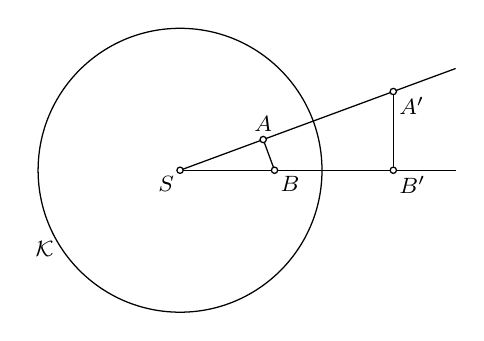
\begin{tikzpicture}
                % \clip (0,0) rectangle (14.000000,10.000000);
                {\footnotesize
                
                % Drawing circle k
                \draw [line width=0.016cm] (4.500000,3.500000) circle (1.802776);%
                
                % Drawing line s
                \draw [line width=0.016cm] (4.540000,3.500000) -- (5.660000,3.500000);%
                \draw [line width=0.016cm] (5.740000,3.500000) -- (7.168333,3.500000);%
                \draw [line width=0.016cm] (7.248333,3.500000) -- (8.000000,3.500000);%
                
                % Drawing line u
                \draw [line width=0.016cm] (7.208333,3.540000) -- (7.208333,4.460001);%

                % Drawing line S B'
                \draw [line width=0.016cm] (4.537523,3.513856) -- (5.518475,3.876099);%
                \draw [line width=0.016cm] (5.593522,3.903812) -- (7.170477,4.486144);%
                \draw [line width=0.016cm] (7.245523,4.513856) -- (8.000000,4.792467);%
                
                % Drawing segment B' A'
                \draw [line width=0.016cm] (5.569855,3.852432) -- (5.686144,3.537523);%
                
                % Marking point S by circle
                \draw [line width=0.016cm] (4.500000,3.500000) circle (0.040000);%
                \draw (4.530000,3.530000) node [anchor=north east] { $S$ };%
                
                % Marking point K
                \draw (3.000000,2.500000) node [anchor=east] { $\mathcal{K}$ };%

                % Marking point B by circle
                \draw [line width=0.016cm] (5.700000,3.500000) circle (0.040000);%
                \draw (5.670000,3.530000) node [anchor=north west] { $B$ };%
                
                % Marking point B' by circle
                \draw [line width=0.016cm] (7.208333,3.500000) circle (0.040000);%
                \draw (7.178333,3.530000) node [anchor=north west] { $B'$ };%
                
                % Marking point A' by circle
                \draw [line width=0.016cm] (7.208000,4.500000) circle (0.040000);%
                \draw (7.178000,4.530000) node [anchor=north west] { $A'$ };%
                
                % Marking point A by circle
                \draw [line width=0.016cm] (5.555999,3.889955) circle (0.040000);%
                \draw (5.555999,3.889955) node [anchor=south] { $A$ };%
                
                }
                \end{tikzpicture}
            \\ Po potenci točke na krožnico velja: $|\tilde{S}A|\cdot|\tilde{S}A'|=r^2=|\tilde{S}B|\cdot|\tilde{S}B'|$. Ker za trikotnika $\triangle\tilde{S}AB$ in $\triangle\tilde{S}B'A'$ velja razmerje $\frac{|\tilde{S}A|}{|\tilde{S}B|}=\frac{|\tilde{S}B'|}{|\tilde{S}A'|}$ in imata skupen kot pri $\tilde{S}$, potem po podobnostnem kriteriju SKS velja: $\triangle\tilde{S}AB\sim\triangle\tilde{S}B'A'$. Od tod pa sledi razmerje: $\frac{|A'B'|}{|AB|}=\frac{|\tilde{S}A'|}{|\tilde{S}B|}$
        \end{dokaz}

    \begin{trditev}
        Naj bo krožnica $\mathcal{K}=K(S,r)$ določa P-model hiperbolične ravnine in naj bi P-premica $p$ del krožnica $\tilde{\mathcal{K}}=K(\tilde{S},\tilde{r})$.
        Potem za poljubni točki $A,B\in\mathcal{H}$ velja $d(A,B)=d(A',B')$, kjer sta $A', B'$ inverza za točki $A, B$ v $\tilde{\mathcal{K}}$.
    \end{trditev}

        \begin{dokaz}
            \\ Naj bosta $\Omega$ in $\Sigma$ idealni točki na P-premici $\overleftrightarrow{AB}$ ter $\Omega'$ $\Sigma'$ njuni sliki pri inverziji v $\tilde{\mathcal{K}}$.
            \\ 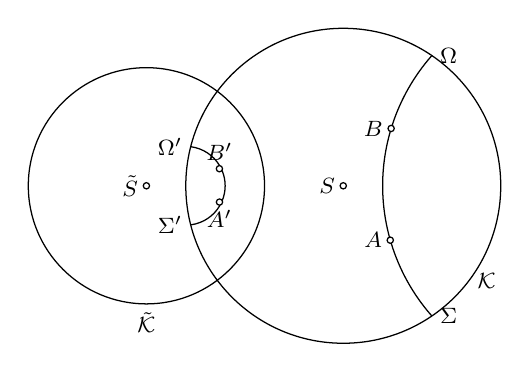
\begin{tikzpicture}
                    % \clip (0,0) rectangle (14.000000,10.000000);
                    {\footnotesize
                    
                    % Drawing circle k
                    \draw [line width=0.016cm] (2.000000,3.500000) circle (1.500000);%
                    
                    % Drawing circle k'
                    \draw [line width=0.016cm] (4.500000,3.500000) circle (2.000000);%
                    
                    % Marking point \tilde{S} by circle
                    \draw [line width=0.016cm] (2.000000,3.500000) circle (0.040000);%
                    \draw (2.000000,3.500000) node [anchor=east] { $\tilde{S}$ };%
                    
                    % Drawing arc S'' U 165.64
                    \draw [line width=0.016cm] (2.562500,3.003922) -- (2.569586,3.004866) arc (278:330:0.500000 and 0.500000) -- (2.935090,3.253633);%
                    \draw [line width=0.016cm] (2.963262,3.311883) -- (2.963592,3.312697) arc (338:360:0.500000 and 0.500000) --(3.000000,3.500000) arc (0:22:0.500000 and 0.500000) -- (2.960407,3.695001);%
                    \draw [line width=0.016cm] (2.928923,3.756954) -- (2.928584,3.757519) arc (31:82:0.500000 and 0.500000) -- (2.562500,3.996078);%
                    
                    % Marking point B' by circle
                    \draw [line width=0.016cm] (2.927000,3.717000) circle (0.040000);%
                    \draw (2.927000,3.717000) node [anchor=south] { $B'$ };%
                    
                    % Marking point A' by circle
                    \draw [line width=0.016cm] (2.928000,3.293000) circle (0.040000);%
                    \draw (2.928000,3.293000) node [anchor=north] { $A'$ };%
                    
                    % Marking point \Omega'
                    \draw (2.562000,3.996000) node [anchor=east] { $\Omega'$ };%
                    
                    % Marking point \Sigma'
                    \draw (2.562000,3.004000) node [anchor=east] { $\Sigma'$ };%
                    
                    % Marking point A by circle
                    \draw [line width=0.016cm] (5.097000,2.809000) circle (0.040000);%
                    \draw (5.097000,2.809000) node [anchor=east] { $A$ };%
                    
                    % Marking point B by circle
                    \draw [line width=0.016cm] (5.108000,4.228000) circle (0.040000);%
                    \draw (5.108000,4.228000) node [anchor=east] { $B$ };%
                    
                    % Marking point \Omega
                    \draw (5.625000,5.153595) node [anchor=west] { $\Omega$ };%
                    
                    % Marking point \Sigma
                    \draw (5.625000,1.846405) node [anchor=west] { $\Sigma$ };%
                    
                    % Drawing arc N \Omega 82.82
                    \draw [line width=0.016cm] (5.625000,5.153595) -- (5.613226,5.140148) arc (139:162:2.500000 and 2.500000) -- (5.120266,4.266073);%
                    \draw [line width=0.016cm] (5.096976,4.189549) -- (5.096846,4.189094) arc (164:195:2.500000 and 2.500000) -- (5.086618,2.847629);%
                    \draw [line width=0.016cm] (5.108723,2.770757) -- (5.109238,2.769071) arc (197:221:2.500000 and 2.500000) -- (5.624999,1.846406);%
                    
                    % Marking point S by circle
                    \draw [line width=0.016cm] (4.500000,3.500000) circle (0.040000);%
                    \draw (4.500000,3.500000) node [anchor=east] { $S$ };%
                    
                    % Marking point \mathcal{K}
                    \draw (6.100000,2.500000) node [anchor=north west] { $\mathcal{K}$ };%
                    
                    % Marking point \tilde{\mathcal{K}}
                    \draw (2.000000,2.000000) node [anchor=north] { $\tilde{\mathcal{K}}$ };%
                    }
                \end{tikzpicture}
            \\ Inverzija v $\tilde{\mathcal{K}}$ slika P-premico $\overleftrightarrow{AB}$ v P-premico $\overleftrightarrow{A'B'}$, saj inverzija slika premice in krožnicee v premice in krožnice ter ohranja velikosti kotov.
            \\ $d(A,B)=\left|\log(AB,\Omega\Sigma)\right|$ in $d(A',B')=\left|\log(A'B',\Omega'\Sigma')\right|$
            \\ Trdimo,da je \dashuline{$(AB,\Omega\Sigma)=(A'B',\Omega'\Sigma')$}, od tod pa sledi $d(A,B)=d(A',B')$.
            \\ $\frac{(AB,\Omega\Sigma)}{(A'B',\Omega'\Sigma')} \rightarrow \frac{\frac{|A'\Omega'|}{|A\Omega|}\cdot\frac{|B'\Sigma'|}{B\Sigma|}}{\frac{|A'\Sigma'|}{|A\Sigma|}\cdot\frac{|B'\Omega'|}{|B\Omega|}}$, po lemi je to enako: $\frac{\frac{|A'\tilde{S}|}{|\tilde{S}\Omega|}\cdot\frac{|B'\tilde{S}|}{\tilde{S}\Sigma|}}{\frac{|A'\tilde{S}|}{|\tilde{S}\Sigma|}\cdot\frac{|B'\tilde{S}|}{|\tilde{S}\Omega|}}=1$.
        \end{dokaz}

    \begin{posledica}
        Inverzija v $\tilde{\mathcal{K}}$ je izometrija $\mathcal{H}$, ki geometrijsko ustreza P-zrcaljenju v P-premici $\tilde{\mathcal{K}}\cap\mathcal{K}$.
    \end{posledica}

    \begin{trditev}
        Zrcaljenje v premici, ki je nosilka premera krožnice $\mathcal{K}$ porodi hiperbolično izometrijo, ki je hiperbolično zrcaljenje v tem premeru.
    \end{trditev}

    Podobno je rotacija s središčem v $S$ (središče $\mathcal{K}$) tudi hiperbolična izometrija.


    \section{Veljavnost aksiomov hiperbolične geometrije v Poincaréjev krožnem modelu}

            
    \subsection*{Aksiomi vsebovanosti}

        \begin{trditev}[V.1]
            Naj bosta $A,B\in\mathcal{H}$. Potem obstaja natanko ena $P$-premica skozi $A$ in $B$ v $\mathcal{H}$.
        \end{trditev}

            \begin{dokaz}
                \\ OBSTOJ:
                \begin{enumerate}
                    \item Če so $A, B, S$ evklidsko kolinearne, potem $A, B$ ležita na nekem premeru, ki je $P$-premica.
                    \item Če $A, B, S$ nisko evklidsko kolinearne. Naj bo $A'=inv_{\mathcal{K}}(A)$. Potem je vsaka krožnica, ki vsebuje $A$ in $A'$, pravokotna na $\mathcal{K}$. Ker $A, A', B$ niso kolinearne, enolično določajo krožnico $\tilde{\mathcal{K}}$, ki je pravokotna na $\mathcal{K}$. Potem je $\mathcal{K}\cap\tilde{\mathcal{K}}$~$P$-premica, ki vsebuje $A$ in $B$.
                \end{enumerate}
                ENOLIČNOST:
                \\ Naj za $A,B$ obstajata dve $P$-premici $p_1$ in $p_2$, ki ju vsebujeta. Ker dve točki enolično določata evklidsko premico, je največ ena izmed $p_1$ in $p_2$ lahko premer.
                \begin{enumerate}
                    \item Naj bo $p_1$ premer in $p_2$ krožni lok. Inverzija v $\mathcal{K}$ slika $A$ v $A'$ in $B$ v $B'$. Ker inverzija v $\mathcal{K}$ slika nosilko premera $p_1$ nazaj vase in krožnico $\tilde{\mathcal{K}}$, ki nosi $p_2$, prav tako nazaj vase, imata premica $p$ in krožnica $\tilde{\mathcal{K}}$ 4 skupne točke. Kar nas privede v protislovje.
                    \item $p_1$ in $p_2$ sta krožna loka. Kot zgoraj sledi, da imata krožnici, ki nosita $p_1$ in $p_2$, 4 skupne točke. Kar je spet protislovje.
                \end{enumerate}
            \end{dokaz}

        \begin{trditev}[V.2]
            Na vsaki $P$-premici ležita vsaj dve različni točki.
        \end{trditev}

        \begin{trditev}[V.3]
            Obstajajo tri različne nekolinearne točke.
        \end{trditev}

        Trditvi V.2 in V.3 očitno veljata.

    \subsection*{Aksiomi vmesnosti}

        \begin{trditev}[M.1]
            Če velja $A\ast B\ast C$, potem velja tudi $C\ast B\ast A$, kjer so $A, B, C$ različne kolinearne točke.
        \end{trditev}

        \begin{trditev}[M.2]
            Naj bosta $B,D\in\mathcal{H}$. Potem obstajajo točke $A,B,C\in\mathcal{H}$ na $P$-premici $AB$, da velja $A\ast B\ast D$, $B\ast C\ast D$ in $B \ast D \ast E$.
        \end{trditev}

        \begin{trditev}[M.3]
            Naj bodo $A,B,C\in\mathcal{H}$. Natanko ena točka leži med drugima dvema, če so točke kolinearne.
        \end{trditev}

        \begin{trditev}[M.4]
            Za poljubno $P$-premico $p$ in točke $A, B, C$, ki ne ležijo na $P$-premici $p$, velja:
            \begin{enumerate}
                \item Če sta $A$ in $B$ na istem bregu $P$-premice $p$ ter $B$ in $C$ na istem bregu $P$-premice $p$, potem sta $A$ in $C$ na istem bregu $P$-premice $p$.
                \item Če sta $A$ in $B$ na različnih bregovih $P$-premice $p$ in $B$ in $C$ na različnih bregovih $P$-premice $p$, potem sta $A$ in $C$ na istem bregu $P$-premice $p$.
            \end{enumerate}
        \end{trditev}
        \begin{dokaz}
            \\ Intuitivno je jasno, da vsaka $P$-premica razdeli $\mathcal{H}$ na dva bregova. Da uskladimo ta pojma, je treba dokazati, da intuitivna delitev ustreza uradni definiciji. Potem pa je verifikacija trditve M.4 dana. Argument za to je zelo podoben tistemu v dokazu trditve V.1.
        \end{dokaz}

    \subsection*{Aksiomi skladnosti}

        \begin{trditev}[S.1]
             Če sta $A$ in $B$ različni točki in $A'$ poljubna točka, potem na poljubnem poltraku $r$ z začetkom v $A'$ obstaja natanko ena točka $B'$, da velja $B'\neq A'$ in $AB\cong A'B'$.
        \end{trditev}

            \begin{dokaz}
                \\ Pokazati je treba, da ima poljuben poltrak neskončno dolžino.
                \\ Poltrak $r$ skozi $A$ je del neke P-premice. Pokazati moramo, da na $r$ obstaja taka točka $b$, da je $d(A,B)$ poljubno veliko. Naj bodo točke $A, \Omega, \Sigma$ fiksirane, $B$ pa lahko potuje od $A$ proti $\Omega$. Potem je: $\lim_{B\to\Omega}d(A,B)=\lim_{B\to\Omega}\left|\log\frac{|A\Omega|\cdot|B\Sigma|}{|A\Sigma|\cdot|B\Omega|}\right|=\infty$.
            \end{dokaz}

        \begin{trditev}[S.2]
            Skladnost daljic je ekvivalenčna relacija.
        \end{trditev}

        Trditev $S.2$ je očitna, saj je enakost, preko katere je definirana skladnost, ekvivalenčna relacija.

        \begin{trditev}[S.3]
            Če velja $A\ast B\ast C$, $A'\ast B'\ast C'$, $AB\cong A'B'$ in $BC\cong B'C'$, potem je $AC\cong A'C'$.
        \end{trditev}

            \begin{dokaz}
                \\ 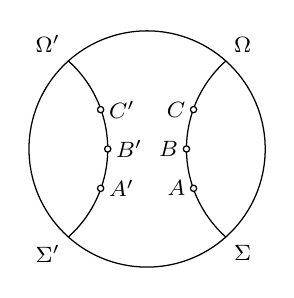
\begin{tikzpicture}
                        % \clip (0,0) rectangle (14.000000,10.000000);
                        {\footnotesize
                        
                        % Drawing circle l
                        \draw [line width=0.016cm] (4.500000,3.000000) circle (1.500000);%
                        
                        % Marking point B by circle
                        \draw [line width=0.016cm] (5.000000,3.000000) circle (0.040000);%
                        \draw (5.000000,3.000000) node [anchor=east] { $B$ };%
                        
                        % Marking point B' by circle
                        \draw [line width=0.016cm] (4.000000,3.000000) circle (0.040000);%
                        \draw (4.000000,3.000000) node [anchor=west] { $B'$ };%
                        
                        % Marking point \Omega
                        \draw (5.500000,4.118034) node [anchor=south west] { $\Omega$ };%
                        
                        % Marking point \Sigma
                        \draw (5.500000,1.881966) node [anchor=north west] { $\Sigma$ };%
                        
                        % Marking point \Omega'
                        \draw (3.500000,4.118034) node [anchor=south east] { $\Omega'$ };%
                        
                        % Marking point \Sigma'
                        \draw (3.500000,1.881966) node [anchor=north east] { $\Sigma'$ };%
                        
                        % Drawing arc P \Omega 96.38
                        \draw [line width=0.016cm] (5.500000,4.118034) -- (5.496304,4.114717) arc (132:158:1.500000 and 1.500000) -- (5.100075,3.538710);%
                        \draw [line width=0.016cm] (5.073436,3.463591) -- (5.073415,3.463526) arc (162:178:1.500000 and 1.500000) -- (5.000533,3.039996);%
                        \draw [line width=0.016cm] (5.000533,2.960004) -- (5.000914,2.947651) arc (182:198:1.500000 and 1.500000) -- (5.073436,2.536410);%
                        \draw [line width=0.016cm] (5.100074,2.461290) -- (5.109224,2.438090) arc (202:228:1.500000 and 1.500000) -- (5.500000,1.881966);%
                        
                        % Drawing arc P' \Sigma' 96.38
                        \draw [line width=0.016cm] (3.500000,1.881966) -- (3.503696,1.885282) arc (312:338:1.500000 and 1.500000) -- (3.899925,2.461289);%
                        \draw [line width=0.016cm] (3.926563,2.536409) -- (3.926585,2.536474) arc (342:358:1.500000 and 1.500000) -- (3.999467,2.960003);%
                        \draw [line width=0.016cm] (3.999467,3.039996) -- (3.999086,3.052349) arc (2:18:1.500000 and 1.500000) -- (3.926564,3.463591);%
                        \draw [line width=0.016cm] (3.899925,3.538710) -- (3.890776,3.561910) arc (22:48:1.500000 and 1.500000) -- (3.500000,4.118034);%
                        
                        % Marking point C' by circle
                        \draw [line width=0.016cm] (3.910000,3.500000) circle (0.040000);%
                        \draw (3.910000,3.500000) node [anchor=west] { $C'$ };%
                        
                        % Marking point A' by circle
                        \draw [line width=0.016cm] (3.910000,2.500000) circle (0.040000);%
                        \draw (3.910000,2.500000) node [anchor=west] { $A'$ };%
                        
                        % Marking point A by circle
                        \draw [line width=0.016cm] (5.090000,2.500000) circle (0.040000);%
                        \draw (5.090000,2.500000) node [anchor=east] { $A$ };%
                        
                        % Marking point C by circle
                        \draw [line width=0.016cm] (5.090000,3.500000) circle (0.040000);%
                        \draw (5.090000,3.500000) node [anchor=east] { $C$ };%
                        }
                    \end{tikzpicture}                    
                \\ $|AB|_H=|A'B'|_H=x$ in $|BC|_H=|B'C'|_H=y$. Dokazujemo: \dashuline{$|AB|_H+|BC|_H=|AC|_H$}.
                % \\ $|AC|_H=\left\lvert \log(AC, \Sigma\Omega)\right\rvert =\left\lvert \log\frac{|A\Sigma|\cdot|C\Omega|}{|A\Omega|\cdot|C\Sigma|}\right\rvert$
                \\ $|AB|_H+|BC|_H=\left\lvert \log\frac{|A\Sigma|\cdot|B\Omega|}{|A\Omega|\cdot|B\Sigma|}\right\rvert+\left\lvert \log\frac{|B\Sigma|\cdot|C\Omega|}{|B\Omega|\cdot|C\Sigma|}\right\rvert=\left\lvert \log\frac{|A\Sigma|\cdot|B\Omega|\cdot|B\Sigma|\cdot|C\Omega|}{|A\Omega|\cdot|B\Sigma|\cdot|C\Sigma|\cdot|B\Omega|}\right\rvert=\left\lvert \log\frac{|A\Sigma|\cdot|C\Omega|}{|A\Omega|\cdot|C\Sigma|}\right\rvert=|AC|_H$
                \\ Enak račun velja za $|A'C'|_H$.
            \end{dokaz}

        \begin{trditev}[S.4]
            Za dani kot $\angle CAB$ in dani poltrak $\overrightarrow{A'B'}$ obstaja natanko en poltrak $\overrightarrow{A'C'}$ na izbranem bregu $\overleftrightarrow{A'B'}$, da je $\angle CAB \cong \angle C'A'B'$.
        \end{trditev}

            \begin{dokaz}
                \\ Označimo: $|\angle CAB|=\alpha$ in glede na izbiro lege točke $A'$ ločimo $2$ primera:
                \\ (1): Če je $A'=O$, na izbranem bregu premice $\overleftrightarrow{A'B'}$ izbremo točko $C'$, ki z dano premico oklepa kot $\alpha$. (enako kot v evklidski geometriji)
                \\ (2): Če je $A'\neq O$. Naj bo $p$ evklidska premica, ki z $\overleftrightarrow{A'B'}$ oklepa  kot $\alpha$. Če je $p$ premer krožnice $\mathcal{K}$, je del premice $p$, ki leži v $\mathcal{H}$, iskana $P$-prmeica. 
                \\ 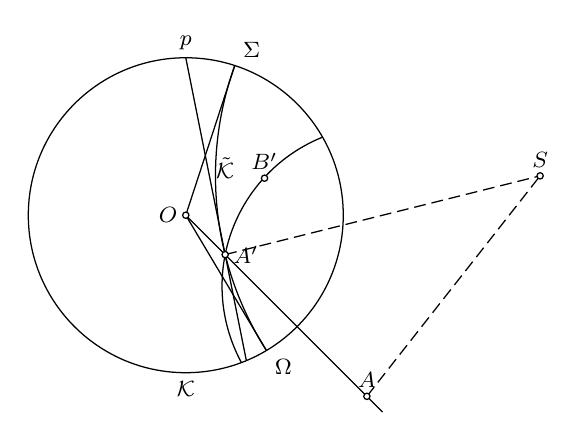
\begin{tikzpicture}
                        % \clip (0,0) rectangle (14.000000,10.000000);
                        {\footnotesize
                        
                        % Drawing circle k
                        \draw [line width=0.016cm] (3.500000,3.500000) circle (2.000000);%
                        
                        % Marking point O by circle
                        \draw [line width=0.016cm] (3.500000,3.500000) circle (0.040000);%
                        \draw (3.500000,3.500000) node [anchor=east] { $O$ };%
                        
                        % Marking point p
                        \draw (3.500000,5.500000) node [anchor=south] { $p$ };%
                        
                        % Marking point A' by circle
                        \draw [line width=0.016cm] (4.000000,3.000000) circle (0.040000);%
                        \draw (4.000000,3.000000) node [anchor=west] { $A'$ };%
                        
                        % Drawing segment D p
                        \draw [line width=0.016cm] (4.269231,1.653846) -- (4.007845,2.960777);%
                        \draw [line width=0.016cm] (3.992155,3.039223) -- (3.500000,5.500000);%
                        
                        % Marking point \Sigma
                        \draw (4.122136,5.400775) node [anchor=south west] { $\Sigma$ };%
                        
                        % Marking point \Omega
                        \draw (4.524205,1.782152) node [anchor=north west] { $\Omega$ };%
                        
                        % Drawing segment O \Sigma
                        \draw [line width=0.016cm] (3.512443,3.538016) -- (4.122136,5.400775);%
                        
                        % Drawing segment O \Omega
                        \draw [line width=0.016cm] (3.520484,3.465643) -- (4.524205,1.782152);%
                        
                        % Marking point B' by circle
                        \draw [line width=0.016cm] (4.500000,3.970000) circle (0.040000);%
                        \draw (4.500000,3.970000) node [anchor=south] { $B'$ };%
                        
                        % Drawing arc S \Sigma 52.40
                        \draw [line width=0.016cm] (4.122136,5.400775) -- (4.101527,5.342352) arc (161:193:4.123106 and 4.123106) -- (3.990487,3.038852);%
                        \draw [line width=0.016cm] (4.009889,2.961243) -- (4.017386,2.932862) arc (195:212:4.123106 and 4.123106) -- (4.524205,1.782153);%
                        
                        % Drawing arc S' \Sigma' 96.46
                        \draw [line width=0.016cm] (5.236936,4.491490) -- (5.235950,4.491091) arc (112:136:2.039608 and 2.039608) -- (4.520739,4.004204);%
                        \draw [line width=0.016cm] (4.467811,3.946253) -- (4.460689,3.938103) arc (139:167:2.039608 and 2.039608) -- (4.008229,3.039144);%
                        \draw [line width=0.016cm] (3.992540,2.960702) -- (3.991378,2.954174) arc (170:208:2.039608 and 2.039608) -- (4.206406,1.628907);%
                        
                        % Marking point A by circle
                        \draw [line width=0.016cm] (5.800000,1.200000) circle (0.040000);%
                        \draw (5.800000,1.200000) node [anchor=south] { $A$ };%
                        
                        % Drawing segment O U
                        \draw [line width=0.016cm] (3.528284,3.471716) -- (3.971716,3.028284);%
                        \draw [line width=0.016cm] (4.028284,2.971716) -- (5.771716,1.228284);%
                        \draw [line width=0.016cm] (5.828284,1.171716) -- (6.000000,1.000000);%
                        
                        % Marking point S by circle
                        \draw [line width=0.016cm] (8.000000,4.000000) circle (0.040000);%
                        \draw (8.000000,4.000000) node [anchor=south] { $S$ };%
                        
                        % Drawing segment A' S
                        \draw [line width=0.016cm] (4.038806,3.009701) -- (4.145521,3.036380);%
                        \draw [line width=0.016cm] (4.218282,3.054571) -- (4.363803,3.090951);%
                        \draw [line width=0.016cm] (4.436564,3.109141) -- (4.582086,3.145521);%
                        \draw [line width=0.016cm] (4.654846,3.163712) -- (4.800368,3.200092);%
                        \draw [line width=0.016cm] (4.873128,3.218282) -- (5.018650,3.254662);%
                        \draw [line width=0.016cm] (5.091410,3.272853) -- (5.236932,3.309233);%
                        \draw [line width=0.016cm] (5.309692,3.327423) -- (5.455214,3.363803);%
                        \draw [line width=0.016cm] (5.527974,3.381994) -- (5.673496,3.418374);%
                        \draw [line width=0.016cm] (5.746257,3.436564) -- (5.891778,3.472944);%
                        \draw [line width=0.016cm] (5.964539,3.491135) -- (6.110060,3.527515);%
                        \draw [line width=0.016cm] (6.182821,3.545705) -- (6.328342,3.582086);%
                        \draw [line width=0.016cm] (6.401103,3.600276) -- (6.546624,3.636656);%
                        \draw [line width=0.016cm] (6.619385,3.654846) -- (6.764906,3.691227);%
                        \draw [line width=0.016cm] (6.837667,3.709417) -- (6.983188,3.745797);%
                        \draw [line width=0.016cm] (7.055949,3.763987) -- (7.201470,3.800368);%
                        \draw [line width=0.016cm] (7.274231,3.818558) -- (7.419752,3.854938);%
                        \draw [line width=0.016cm] (7.492513,3.873128) -- (7.638034,3.909509);%
                        \draw [line width=0.016cm] (7.710795,3.927699) -- (7.856316,3.964079);%
                        \draw [line width=0.016cm] (7.929077,3.982269) -- (7.961194,3.990299);%
                        
                        % Drawing segment A S
                        \draw [line width=0.016cm] (5.824713,1.231453) -- (5.892673,1.317948);%
                        \draw [line width=0.016cm] (5.939010,1.376922) -- (6.031683,1.494869);%
                        \draw [line width=0.016cm] (6.078020,1.553843) -- (6.170693,1.671791);%
                        \draw [line width=0.016cm] (6.217030,1.730765) -- (6.309703,1.848713);%
                        \draw [line width=0.016cm] (6.356039,1.907687) -- (6.448713,2.025634);%
                        \draw [line width=0.016cm] (6.495049,2.084608) -- (6.587722,2.202556);%
                        \draw [line width=0.016cm] (6.634059,2.261530) -- (6.726732,2.379478);%
                        \draw [line width=0.016cm] (6.773069,2.438451) -- (6.865742,2.556399);%
                        \draw [line width=0.016cm] (6.912079,2.615373) -- (7.004752,2.733321);%
                        \draw [line width=0.016cm] (7.051089,2.792295) -- (7.143762,2.910242);%
                        \draw [line width=0.016cm] (7.190098,2.969216) -- (7.282772,3.087164);%
                        \draw [line width=0.016cm] (7.329108,3.146138) -- (7.421782,3.264086);%
                        \draw [line width=0.016cm] (7.468118,3.323060) -- (7.560791,3.441007);%
                        \draw [line width=0.016cm] (7.607128,3.499981) -- (7.699801,3.617929);%
                        \draw [line width=0.016cm] (7.746138,3.676903) -- (7.838811,3.794851);%
                        \draw [line width=0.016cm] (7.885148,3.853824) -- (7.975287,3.968547);%
                        
                        % Marking point \mathcal{K}
                        \draw (3.500000,1.300000) node  { $\mathcal{K}$ };%

                        % Marking point \tilde{\mathcal{K}}
                        \draw (4.000000,4.100000) node  { $\tilde{\mathcal{K}}$ };%
                        }
                    \end{tikzpicture}                    
                \\ Sicer moramo poiskati krožnico ima premico $p$ za tangento in seka krožnico $\mathcal{K}$ pravokotno. Središče iskane krožnice leži na pravokotnici skozi točko $A'$ na premico $p$. Naj bo $A=inv_{\mathcal{K}}(A')$ in $S$ presečišče pravokotnice na $p$ skozi $A'$ in daljice $AA'$. Po definiciji inverzije je $|OA'|\cdot|OA|=1$. Potenca točke na krožnico nam da: $\mathcal{P}_{\tilde{\mathcal{K}}}(O)=1=|O\Sigma|^2=|O\Omega|^2$. Potem sta $\overleftrightarrow{O\Sigma}$ in $\overleftrightarrow{O\Omega}$ tangentni na krožnico $\tilde{\mathcal{K}}$.
            \end{dokaz}
        
        \begin{trditev}[S.5]
            Skladnost kotov je ekvivalenčna relacija.
        \end{trditev}

        Trditev $S.5$ je očitna, saj je enakost, preko katere je definirana skladnost, ekvivalenčna relacija.

        \begin{trditev}[S.6/SKS]
             Če sta stranici in vmesni kot enega trikotnika skladni s stranicama in vmesnim kotom drugega trikotnika, potem sta trikotnika skladna.
        \end{trditev}

        To trditev bomo preverili tako, da bomo poljuben trikotnik prestavili v posebno lego.
         
        Način, kako trikotnik prestavimo, mora biti tak, da bo P-premice slikal v P-premice in da bo ohranjal razdalje in kote -- izometrija. 
        \\ To lahko storimo z inverzijo v poljubni krožnici $\tilde{\mathcal{K}}$, ki je pravokotna na $\mathcal{K}$.
        $inv_{\tilde{\mathcal{K}}}$ porodi bijekcijo $\mathcal{H}\to\mathcal{H}$, ki fiksira točke na P-premici $\tilde{\mathcal{K}}\cap\mathcal{K}$. To bo hiperbolično zrcaljenje. 
        \\ Preveriti je potrebno še, da ohranja P-dolžino. Poleg prej obravnavanih izometrij, lahko uporabimo tudi evklidske izometrije, če le-te ohranjajo množico $\mathcal{H}$. Vsaka taka porodi bijekcijo $\mathcal{H}\to\mathcal{H}$, ki ohranja velikosti kotov in evklidske razdalje, zato pa posledično ohranja hiperbolične razdalje.
        \\ Z uporabo teh izometrij bomo poljuben P-trikotnik preslikali na skladen trikotnik v odlikovani legi.
        

            \begin{dokaz}
                \\ Naj bo $\triangle ABC$ poljuben P-trikotnik. (trikotnik preslikamo v skladen trikotnik $\triangle SB'C'$) 
                \\ 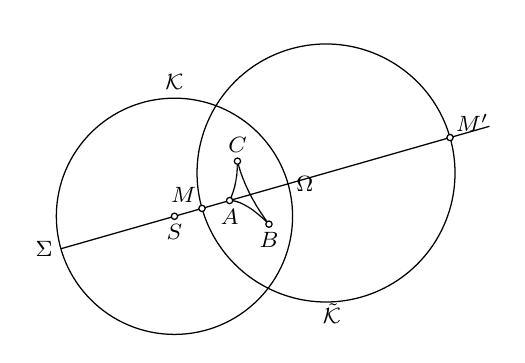
\begin{tikzpicture}
                        % \clip (0,0) rectangle (14.000000,10.000000);
                        {\footnotesize
                        
                        % Marking point S by circle
                        \draw [line width=0.016cm] (3.000000,3.000000) circle (0.040000);%
                        \draw (3.000000,3.000000) node [anchor=north] { $S$ };%
                        
                        % Drawing circle k
                        \draw [line width=0.016cm] (3.000000,3.000000) circle (1.500000);%
                        
                        % Marking point A by circle
                        \draw [line width=0.016cm] (3.700000,3.200000) circle (0.040000);%
                        \draw (3.700000,3.200000) node [anchor=north] { $A$ };%
                        
                        % Marking point M by circle
                        \draw [line width=0.016cm] (3.350000,3.100000) circle (0.040000);%
                        \draw (3.380000,3.070000) node [anchor=south east] { $M$ };%
                        
                        % Marking point \Sigma
                        \draw (1.557714,2.587918) node [anchor=east] { $\Sigma$ };%
                        
                        % Marking point \Omega
                        \draw (4.442286,3.412082) node [anchor=west] { $\Omega$ };%
                        
                        % Marking point M' by circle
                        \draw [line width=0.016cm] (6.500000,4.000000) circle (0.040000);%
                        \draw (6.470000,3.970000) node [anchor=south west] { $M'$ };%
                        
                        % Drawing circle k'
                        \draw [line width=0.016cm] (6.563025,3.549999) arc (360:360:1.638025 and 1.638025) --(6.563025,3.550000) arc (0:14:1.638025 and 1.638025) -- (6.510518,3.961408);%
                        \draw [line width=0.016cm] (6.488542,4.038324) -- (6.482854,4.056177) arc (18:194:1.638025 and 1.638025) -- (3.339481,3.138593);%
                        \draw [line width=0.016cm] (3.361457,3.061677) -- (3.367146,3.043823) arc (198:359:1.638025 and 1.638025) -- (6.563025,3.549999);%
                        
                        % Marking point C by circle
                        \draw [line width=0.016cm] (3.800000,3.700000) circle (0.040000);%
                        \draw (3.800000,3.700000) node [anchor=south] { $C$ };%
                        
                        % Marking point B by circle
                        \draw [line width=0.016cm] (4.200000,2.900000) circle (0.040000);%
                        \draw (4.200000,2.900000) node [anchor=north] { $B$ };%
                        
                        % Drawing Bezier curve A X C
                        \draw [line width=0.016cm] (3.720988,3.245679) -- (3.716926,3.236243);%
                        \draw [line width=0.016cm] (3.725849,3.257485) -- (3.720988,3.245679);%
                        \draw [line width=0.016cm] (3.730556,3.269444) -- (3.725849,3.257485);%
                        \draw [line width=0.016cm] (3.735108,3.281559) -- (3.730556,3.269444);%
                        \draw [line width=0.016cm] (3.739506,3.293827) -- (3.735108,3.281559);%
                        \draw [line width=0.016cm] (3.743750,3.306250) -- (3.739506,3.293827);%
                        \draw [line width=0.016cm] (3.747840,3.318827) -- (3.743750,3.306250);%
                        \draw [line width=0.016cm] (3.751775,3.331559) -- (3.747840,3.318827);%
                        \draw [line width=0.016cm] (3.755556,3.344444) -- (3.751775,3.331559);%
                        \draw [line width=0.016cm] (3.759182,3.357485) -- (3.755556,3.344444);%
                        \draw [line width=0.016cm] (3.762654,3.370679) -- (3.759182,3.357485);%
                        \draw [line width=0.016cm] (3.765972,3.384028) -- (3.762654,3.370679);%
                        \draw [line width=0.016cm] (3.769136,3.397531) -- (3.765972,3.384028);%
                        \draw [line width=0.016cm] (3.772145,3.411188) -- (3.769136,3.397531);%
                        \draw [line width=0.016cm] (3.775000,3.425000) -- (3.772145,3.411188);%
                        \draw [line width=0.016cm] (3.777701,3.438966) -- (3.775000,3.425000);%
                        \draw [line width=0.016cm] (3.780247,3.453086) -- (3.777701,3.438966);%
                        \draw [line width=0.016cm] (3.782639,3.467361) -- (3.780247,3.453086);%
                        \draw [line width=0.016cm] (3.784877,3.481790) -- (3.782639,3.467361);%
                        \draw [line width=0.016cm] (3.786960,3.496373) -- (3.784877,3.481790);%
                        \draw [line width=0.016cm] (3.788889,3.511111) -- (3.786960,3.496373);%
                        \draw [line width=0.016cm] (3.790664,3.526003) -- (3.788889,3.511111);%
                        \draw [line width=0.016cm] (3.792284,3.541049) -- (3.790664,3.526003);%
                        \draw [line width=0.016cm] (3.793750,3.556250) -- (3.792284,3.541049);%
                        \draw [line width=0.016cm] (3.795062,3.571605) -- (3.793750,3.556250);%
                        \draw [line width=0.016cm] (3.796219,3.587114) -- (3.795062,3.571605);%
                        \draw [line width=0.016cm] (3.797222,3.602778) -- (3.796219,3.587114);%
                        \draw [line width=0.016cm] (3.798071,3.618596) -- (3.797222,3.602778);%
                        \draw [line width=0.016cm] (3.798765,3.634568) -- (3.798071,3.618596);%
                        \draw [line width=0.016cm] (3.799306,3.650694) -- (3.798765,3.634568);%
                        \draw [line width=0.016cm] (3.799526,3.660003) -- (3.799306,3.650694);%
                        
                        % Drawing Bezier curve A Y B
                        \draw [line width=0.016cm] (3.745679,3.196296) -- (3.739895,3.197101);%
                        \draw [line width=0.016cm] (3.757485,3.194213) -- (3.745679,3.196296);%
                        \draw [line width=0.016cm] (3.769444,3.191667) -- (3.757485,3.194213);%
                        \draw [line width=0.016cm] (3.781559,3.188657) -- (3.769444,3.191667);%
                        \draw [line width=0.016cm] (3.793827,3.185185) -- (3.781559,3.188657);%
                        \draw [line width=0.016cm] (3.806250,3.181250) -- (3.793827,3.185185);%
                        \draw [line width=0.016cm] (3.818827,3.176852) -- (3.806250,3.181250);%
                        \draw [line width=0.016cm] (3.831559,3.171991) -- (3.818827,3.176852);%
                        \draw [line width=0.016cm] (3.844444,3.166667) -- (3.831559,3.171991);%
                        \draw [line width=0.016cm] (3.857485,3.160880) -- (3.844444,3.166667);%
                        \draw [line width=0.016cm] (3.870679,3.154630) -- (3.857485,3.160880);%
                        \draw [line width=0.016cm] (3.884028,3.147917) -- (3.870679,3.154630);%
                        \draw [line width=0.016cm] (3.897531,3.140741) -- (3.884028,3.147917);%
                        \draw [line width=0.016cm] (3.911188,3.133102) -- (3.897531,3.140741);%
                        \draw [line width=0.016cm] (3.925000,3.125000) -- (3.911188,3.133102);%
                        \draw [line width=0.016cm] (3.938966,3.116435) -- (3.925000,3.125000);%
                        \draw [line width=0.016cm] (3.953086,3.107407) -- (3.938966,3.116435);%
                        \draw [line width=0.016cm] (3.967361,3.097917) -- (3.953086,3.107407);%
                        \draw [line width=0.016cm] (3.981790,3.087963) -- (3.967361,3.097917);%
                        \draw [line width=0.016cm] (3.996373,3.077546) -- (3.981790,3.087963);%
                        \draw [line width=0.016cm] (4.011111,3.066667) -- (3.996373,3.077546);%
                        \draw [line width=0.016cm] (4.026003,3.055324) -- (4.011111,3.066667);%
                        \draw [line width=0.016cm] (4.041049,3.043519) -- (4.026003,3.055324);%
                        \draw [line width=0.016cm] (4.056250,3.031250) -- (4.041049,3.043519);%
                        \draw [line width=0.016cm] (4.071605,3.018519) -- (4.056250,3.031250);%
                        \draw [line width=0.016cm] (4.087114,3.005324) -- (4.071605,3.018519);%
                        \draw [line width=0.016cm] (4.102778,2.991667) -- (4.087114,3.005324);%
                        \draw [line width=0.016cm] (4.118596,2.977546) -- (4.102778,2.991667);%
                        \draw [line width=0.016cm] (4.134568,2.962963) -- (4.118596,2.977546);%
                        \draw [line width=0.016cm] (4.150694,2.947917) -- (4.134568,2.962963);%
                        \draw [line width=0.016cm] (4.166975,2.932407) -- (4.150694,2.947917);%
                        \draw [line width=0.016cm] (4.171471,2.928038) -- (4.166975,2.932407);%
                        
                        % Drawing Bezier curve C Z B
                        \draw [line width=0.016cm] (3.811728,3.655556) -- (3.810169,3.661314);%
                        \draw [line width=0.016cm] (3.818056,3.633333) -- (3.811728,3.655556);%
                        \draw [line width=0.016cm] (3.824691,3.611111) -- (3.818056,3.633333);%
                        \draw [line width=0.016cm] (3.831636,3.588889) -- (3.824691,3.611111);%
                        \draw [line width=0.016cm] (3.838889,3.566667) -- (3.831636,3.588889);%
                        \draw [line width=0.016cm] (3.846451,3.544444) -- (3.838889,3.566667);%
                        \draw [line width=0.016cm] (3.854321,3.522222) -- (3.846451,3.544444);%
                        \draw [line width=0.016cm] (3.862500,3.500000) -- (3.854321,3.522222);%
                        \draw [line width=0.016cm] (3.870988,3.477778) -- (3.862500,3.500000);%
                        \draw [line width=0.016cm] (3.879784,3.455556) -- (3.870988,3.477778);%
                        \draw [line width=0.016cm] (3.888889,3.433333) -- (3.879784,3.455556);%
                        \draw [line width=0.016cm] (3.898302,3.411111) -- (3.888889,3.433333);%
                        \draw [line width=0.016cm] (3.908025,3.388889) -- (3.898302,3.411111);%
                        \draw [line width=0.016cm] (3.918056,3.366667) -- (3.908025,3.388889);%
                        \draw [line width=0.016cm] (3.928395,3.344444) -- (3.918056,3.366667);%
                        \draw [line width=0.016cm] (3.939043,3.322222) -- (3.928395,3.344444);%
                        \draw [line width=0.016cm] (3.950000,3.300000) -- (3.939043,3.322222);%
                        \draw [line width=0.016cm] (3.961265,3.277778) -- (3.950000,3.300000);%
                        \draw [line width=0.016cm] (3.972840,3.255556) -- (3.961265,3.277778);%
                        \draw [line width=0.016cm] (3.984722,3.233333) -- (3.972840,3.255556);%
                        \draw [line width=0.016cm] (3.996914,3.211111) -- (3.984722,3.233333);%
                        \draw [line width=0.016cm] (4.009414,3.188889) -- (3.996914,3.211111);%
                        \draw [line width=0.016cm] (4.022222,3.166667) -- (4.009414,3.188889);%
                        \draw [line width=0.016cm] (4.035340,3.144444) -- (4.022222,3.166667);%
                        \draw [line width=0.016cm] (4.048765,3.122222) -- (4.035340,3.144444);%
                        \draw [line width=0.016cm] (4.062500,3.100000) -- (4.048765,3.122222);%
                        \draw [line width=0.016cm] (4.076543,3.077778) -- (4.062500,3.100000);%
                        \draw [line width=0.016cm] (4.090895,3.055556) -- (4.076543,3.077778);%
                        \draw [line width=0.016cm] (4.105556,3.033333) -- (4.090895,3.055556);%
                        \draw [line width=0.016cm] (4.120525,3.011111) -- (4.105556,3.033333);%
                        \draw [line width=0.016cm] (4.135802,2.988889) -- (4.120525,3.011111);%
                        \draw [line width=0.016cm] (4.151389,2.966667) -- (4.135802,2.988889);%
                        \draw [line width=0.016cm] (4.167284,2.944444) -- (4.151389,2.966667);%
                        \draw [line width=0.016cm] (4.176232,2.932173) -- (4.167284,2.944444);%
                        
                        % Drawing segment \Sigma U
                        \draw [line width=0.016cm] (1.557714,2.587918) -- (2.961539,2.989011);%
                        \draw [line width=0.016cm] (3.038461,3.010989) -- (3.311539,3.089011);%
                        \draw [line width=0.016cm] (3.388461,3.110989) -- (3.661539,3.189011);%
                        \draw [line width=0.016cm] (3.738461,3.210989) -- (6.461539,3.989011);%
                        \draw [line width=0.016cm] (6.538461,4.010989) -- (7.000000,4.142857);%
                        
                        % Marking point \mathcal{K}
                        \draw (3.000000,4.500000) node [anchor=south] { $\mathcal{K}$ };%
                        
                        % Marking point \tilde{\mathcal{K}}
                        \draw (5.000000,2.000000) node [anchor=north] { $\tilde{\mathcal{K}}$ };%
                        }
                    \end{tikzpicture}
                \\ Naj bo $M$ razpolovišče daljice $SA$, torej tista točka na evklidski premici $\overleftrightarrow{SA}$, za katero je $d(SM)=\frac{1}{2}d(SA)$. Da določimo $M$, moramo evklidsko razdlajo $|SM|=d$ izraziti s pomočjo evklidske dolžine $|SA|=a$. Z upoštevanjem $|S\Omega|=|S\Sigma|=r$ (polmer $\mathcal{K}$) dobimo: $|A\Omega|=r-a;~|A\Sigma|=r+a;~|M\Omega|=r-d;~|M\Sigma|=r+d$. Velja: $\left| \log(SM,\Omega\Sigma)\right|=d(SM)=\frac{1}{2}d(SA)=\frac{1}{2}\left|\log(SA,\Omega\Sigma)\right|$. Zaradi izbire $\Omega$ in $\Sigma$ lahko izpustimo absolutno vrednost $|\cdot|$, nato antilogaritmiramo in dobimo: $(SA,\Omega\Sigma)=(SM,\Omega\Sigma)^2$. To enakost lahko poračunamo:
                \\ \begin{align*}
                \frac{r+a}{r-a}&=\left( \frac{r+d}{r-d}\right)^2  ~~/d=ka\\
                \frac{r+a}{r-a}&=\left( \frac{r+ka}{r-ka}\right)^2 \\
                (r+a)(r-ka)^2&=(r-a)(r+ka)^2 \\
                2r^2a+2k^2a^3-4akr^2&=0  ~~/:2a \\
                a^2k^2-2kr^2+r^2&=0  ~~/:a^2 \\
                k^2-2k\left(\frac{r}{a}\right)^2+\left(\frac{r}{a}\right)^2&=0
                \end{align*}
                Od tod sledi $k=\left(\frac{r}{a}\right)^2\left( 1 \pm \sqrt{1-\left(\frac{a}{r}\right)^2} \right)$. Ker pa mora glede na hiperbolično razdaljo veljati $\frac{1}{2}<k<1$, potem sledi, da je $k=\left(\frac{r}{a}\right)^2\left( 1 - \sqrt{1-\left(\frac{a}{r}\right)^2} \right)$. Z uporabo razvoja v vrsto, dobimo $k=\frac{1}{2}+\frac{1}{8}\left(\frac{a}{r}\right)^2+\cdots$.
                \\ Naj bo $M'$ inverz točke $M$ v $\mathcal{K}$ in $\tilde{\mathcal{K}}$ krožnica s premerom $MM'$. Potem je $\mathcal{K}\perp\tilde{\mathcal{K}}$, in ker je inverzija v $\mathcal{K}$ izometrija $\mathcal{H}$, preslika točko $A$ v točko $S$. Označimo s $C'$ in $B'$ inverza točk $C$ in $B$ v $\tilde{\mathcal{K}}$. Potem velja naslednja P-skladnost $\triangle SB'C'\sim\triangle ABC$.
                \\ Z vrtenjem okoli točke $S$ lahko točko $B'$ spravimo na pozitivni poltrak vodoravne osi skozi $S$. Če slika $C'$ pri tem pristane v spodnji polravnini, uporabimo še evklidsko zrcaljenje v vodoravnem premeru, da jo preslikamo v zgornjo polravnino. Tako dobimo P-trikotnik $\triangle SB''C''$, ki je P-skladen s trikotnikom $\triangle ABC$.
                \\ 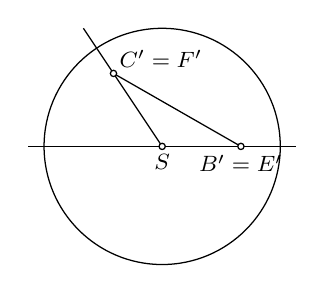
\begin{tikzpicture}
                        % \clip (0,0) rectangle (14.000000,10.000000);
                        {\footnotesize
                        
                        % Marking point S by circle
                        \draw [line width=0.016cm] (3.000000,3.000000) circle (0.040000);%
                        \draw (3.000000,3.000000) node [anchor=north] { $S$ };%
                        
                        % Drawing circle k
                        \draw [line width=0.016cm] (3.000000,3.000000) circle (1.500000);%
                        
                        % Drawing line b
                        \draw [line width=0.016cm] (1.300000,3.000000) -- (2.960000,3.000000);%
                        \draw [line width=0.016cm] (3.040000,3.000000) -- (3.960000,3.000000);%
                        \draw [line width=0.016cm] (4.040000,3.000000) -- (4.700000,3.000000);%
                        
                        % Drawing segment S C
                        \draw [line width=0.016cm] (2.977812,3.033282) -- (2.404188,3.893718);%
                        \draw [line width=0.016cm] (2.359812,3.960282) -- (2.000000,4.500000);%
                        
                        % Marking point C'=F' by circle
                        \draw [line width=0.016cm] (2.382000,3.927000) circle (0.040000);%
                        \draw (2.352000,3.897000) node [anchor=south west] { $C'=F'$ };%
                        
                        % Marking point B'=E' by circle
                        \draw [line width=0.016cm] (4.000000,3.000000) circle (0.040000);%
                        \draw (4.000000,3.000000) node [anchor=north] { $B'=E'$ };%
                        
                        % Drawing segment C'=F' B'=E'
                        \draw [line width=0.016cm] (2.416707,3.907115) -- (3.965293,3.019885);%
                        }
                    \end{tikzpicture}                    
                \\ Če je za nek trikotnik $\triangle DEF$ velja: $\triangle DEF\cong\triangle ABC$, potem ga lahko na enak način preslikamo v trikotnik $\triangle SE'F'$. Velja: $SE'\cong DE\cong AB\cong SB'' \Rightarrow E'=B''$. Ker za kota velja $\angle D\cong \angle A$, sta v trikotnikih $\triangle SB''C''$ in $\triangle SE'F'$ skladna kota pri $S$, zato za poltraka velja: $\overrightarrow{SC''}=\overrightarrow{SF'}$ in kot prej velja $SC''\cong SF' \Rightarrow C''=F'$. To pomeni, da soupadata tudi daljici $B''C''$ in $E'F'$ v teh trikotnikih. Sklep: $\triangle ABC \cong \triangle SB''C''\cong \triangle SE'F'\cong \triangle DEF$.
            \end{dokaz}

        \begin{posledica}
           Dva P-trikotnika sta skladna natanko tedaj, ko obstaja izometrija, ki enega preslika na drugega.
           Ta izometrija je kompozitum P-zrcaljenj (= inverzije v P-premicah), evklidskih zrcaljenj v premerih $\mathcal{K}$ in vrtenj okoli središča $\mathcal{K}$.
        \end{posledica}

\section{Kot vzporednosti v Poincaréjevem modelu}

    \begin{izrek}
        V Poincaréjevem modelu za kot vzporednosti velja: $\tan\left(\frac{\Pi(d)}{2}\right)=e^{-d}$, kjer je $d=d(A,p)$.
    \end{izrek}

        \begin{dokaz}
            \\ Za dano premico $p$ in točko $A\notin p$ asimptotična poltraka iz $A$ oklepata s pravokotnico iz $A$ na $p$ kot, ki ga imenujemo kot vzporednosti $\Pi(A,p)$. Pokazali smo že, da je ta odvisen le od oddaljenosti $A$ od $p$. Naj bo $d=d(AA')$ in $\Pi(A,p)=\Pi(d)$, kjer je $A'$ pravokotna projekcija $A$ na $p$. $\Pi(d)$ bomo izračunali tako, da bomo izbrali posebno lego za $p$ in $A$.
            \\ Naj bo $p$ premer $\mathcal{K}$ in $A$ nad $S$ taka točka, da je $d(AS)=d$. Asimptotičen poltrak skozi $A$ k $p$ je krožni lok na krožnici $\tilde{\mathcal{K}}$ skozi $A$ in $\Omega$, ki je v $\Omega$ pravokoten na $\mathcal{K}$. Središče $\tilde{S}$ krožnice $\tilde{\mathcal{K}}$ je presečišče simetrale daljice $A\Omega$ in pravokotnice na $p$ v $\Omega$.
            \\ 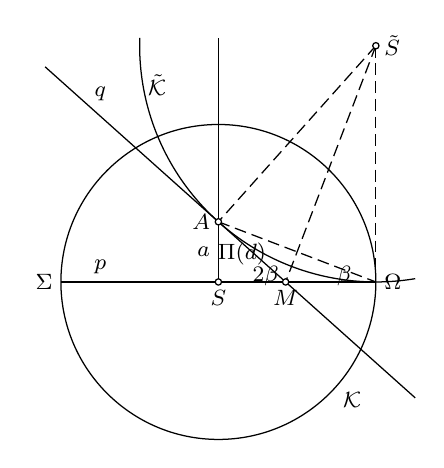
\begin{tikzpicture}
                    % \clip (0,0) rectangle (14.000000,10.000000);
                    {\footnotesize
                    
                    % Drawing circle k
                    \draw [line width=0.016cm] (3.500000,3.500000) circle (2.000000);%
                    
                    % Marking point S by circle
                    \draw [line width=0.016cm] (3.500000,3.500000) circle (0.040000);%
                    \draw (3.500000,3.500000) node [anchor=north] { $S$ };%
                    
                    % Marking point \Sigma
                    \draw (1.500000,3.500000) node [anchor=east] { $\Sigma$ };%
                    
                    % Marking point \Omega
                    \draw (5.500000,3.500000) node [anchor=west] { $\Omega$ };%
                    
                    % Marking point \tilde{S} by circle
                    \draw [line width=0.016cm] (5.500000,6.500000) circle (0.040000);%
                    \draw (5.500000,6.500000) node [anchor=west] { $\tilde{S}$ };%
                    
                    % Drawing circle k'
                    \draw [line width=0.016cm] (2.501667,6.600000) -- (2.500457,6.552358) arc (179:227:3.000000 and 3.000000) -- (3.470364,4.290797);%
                    \draw [line width=0.016cm] (3.529991,4.237465) -- (3.531822,4.235872) arc (229:279:3.000000 and 3.000000) -- (5.999998,3.541960);%
                    
                    % Marking point A by circle
                    \draw [line width=0.016cm] (3.500000,4.263932) circle (0.040000);%
                    \draw (3.500000,4.263932) node [anchor=east] { $A$ };%
                    
                    % Drawing segment S X
                    \draw [line width=0.016cm] (3.500000,3.540000) -- (3.500000,4.223932);%
                    \draw [line width=0.016cm] (3.500000,4.303932) -- (3.500000,6.600000);%
                    
                    % Drawing line q'
                    \draw [line width=0.016cm] (1.300000,6.231672) -- (3.470186,4.290599);%
                    \draw [line width=0.016cm] (3.529814,4.237265) -- (4.324288,3.526667);%
                    \draw [line width=0.016cm] (4.383916,3.473333) -- (6.000000,2.027864);%
                    
                    % Drawing segment \Sigma \Omega
                    \draw [line width=0.016cm] (1.500000,3.500000) -- (3.460000,3.500000);%
                    \draw [line width=0.016cm] (3.540000,3.500000) -- (4.314102,3.500000);%
                    \draw [line width=0.016cm] (4.394102,3.500000) -- (5.500000,3.500000);%
                    
                    % Marking point M by circle
                    \draw [line width=0.016cm] (4.354102,3.500000) circle (0.040000);%
                    \draw (4.354102,3.500000) node [anchor=north] { $M$ };%
                    
                    % Drawing segment \tilde{S} A
                    \draw [line width=0.016cm] (5.473333,6.470186) -- (5.400000,6.388197);%
                    \draw [line width=0.016cm] (5.350000,6.332295) -- (5.250000,6.220492);%
                    \draw [line width=0.016cm] (5.200000,6.164590) -- (5.100000,6.052786);%
                    \draw [line width=0.016cm] (5.050000,5.996885) -- (4.950000,5.885081);%
                    \draw [line width=0.016cm] (4.900000,5.829180) -- (4.800000,5.717376);%
                    \draw [line width=0.016cm] (4.750000,5.661475) -- (4.650000,5.549671);%
                    \draw [line width=0.016cm] (4.600000,5.493769) -- (4.500000,5.381966);%
                    \draw [line width=0.016cm] (4.450000,5.326064) -- (4.350000,5.214261);%
                    \draw [line width=0.016cm] (4.300000,5.158359) -- (4.200000,5.046556);%
                    \draw [line width=0.016cm] (4.150000,4.990654) -- (4.050000,4.878851);%
                    \draw [line width=0.016cm] (4.000000,4.822949) -- (3.900000,4.711146);%
                    \draw [line width=0.016cm] (3.850000,4.655244) -- (3.750000,4.543441);%
                    \draw [line width=0.016cm] (3.700000,4.487539) -- (3.600000,4.375735);%
                    \draw [line width=0.016cm] (3.550000,4.319834) -- (3.526667,4.293746);%
                    
                    % Drawing segment \tilde{S} \Omega
                    \draw [line width=0.016cm] (5.500000,6.460000) -- (5.500000,6.350000);%
                    \draw [line width=0.016cm] (5.500000,6.275000) -- (5.500000,6.125000);%
                    \draw [line width=0.016cm] (5.500000,6.050000) -- (5.500000,5.900000);%
                    \draw [line width=0.016cm] (5.500000,5.825000) -- (5.500000,5.675000);%
                    \draw [line width=0.016cm] (5.500000,5.600000) -- (5.500000,5.450000);%
                    \draw [line width=0.016cm] (5.500000,5.375000) -- (5.500000,5.225000);%
                    \draw [line width=0.016cm] (5.500000,5.150000) -- (5.500000,5.000000);%
                    \draw [line width=0.016cm] (5.500000,4.925000) -- (5.500000,4.775000);%
                    \draw [line width=0.016cm] (5.500000,4.700000) -- (5.500000,4.550000);%
                    \draw [line width=0.016cm] (5.500000,4.475000) -- (5.500000,4.325000);%
                    \draw [line width=0.016cm] (5.500000,4.250000) -- (5.500000,4.100000);%
                    \draw [line width=0.016cm] (5.500000,4.025000) -- (5.500000,3.875000);%
                    \draw [line width=0.016cm] (5.500000,3.800000) -- (5.500000,3.650000);%
                    \draw [line width=0.016cm] (5.500000,3.575000) -- (5.500000,3.500000);%
                    
                    % Drawing segment \tilde{S} M
                    \draw [line width=0.016cm] (5.485727,6.462633) -- (5.446477,6.359874);%
                    \draw [line width=0.016cm] (5.419715,6.289811) -- (5.366192,6.149685);%
                    \draw [line width=0.016cm] (5.339430,6.079622) -- (5.285907,5.939497);%
                    \draw [line width=0.016cm] (5.259145,5.869434) -- (5.205622,5.729308);%
                    \draw [line width=0.016cm] (5.178860,5.659245) -- (5.125337,5.519119);%
                    \draw [line width=0.016cm] (5.098575,5.449056) -- (5.045052,5.308930);%
                    \draw [line width=0.016cm] (5.018290,5.238867) -- (4.964767,5.098741);%
                    \draw [line width=0.016cm] (4.938005,5.028679) -- (4.884482,4.888553);%
                    \draw [line width=0.016cm] (4.857720,4.818490) -- (4.804197,4.678364);%
                    \draw [line width=0.016cm] (4.777435,4.608301) -- (4.723912,4.468175);%
                    \draw [line width=0.016cm] (4.697150,4.398112) -- (4.643627,4.257986);%
                    \draw [line width=0.016cm] (4.616865,4.187923) -- (4.563342,4.047798);%
                    \draw [line width=0.016cm] (4.536580,3.977735) -- (4.483057,3.837609);%
                    \draw [line width=0.016cm] (4.456295,3.767546) -- (4.402772,3.627420);%
                    \draw [line width=0.016cm] (4.376010,3.557357) -- (4.368375,3.537367);%
                    
                    % Drawing segment A \Omega
                    \draw [line width=0.016cm] (3.537367,4.249659) -- (3.640126,4.210409);%
                    \draw [line width=0.016cm] (3.710189,4.183647) -- (3.850315,4.130124);%
                    \draw [line width=0.016cm] (3.920378,4.103362) -- (4.060503,4.049839);%
                    \draw [line width=0.016cm] (4.130566,4.023077) -- (4.270692,3.969554);%
                    \draw [line width=0.016cm] (4.340755,3.942792) -- (4.480881,3.889269);%
                    \draw [line width=0.016cm] (4.550944,3.862507) -- (4.691070,3.808984);%
                    \draw [line width=0.016cm] (4.761133,3.782222) -- (4.901259,3.728699);%
                    \draw [line width=0.016cm] (4.971321,3.701937) -- (5.111447,3.648414);%
                    \draw [line width=0.016cm] (5.181510,3.621652) -- (5.321636,3.568129);%
                    \draw [line width=0.016cm] (5.391699,3.541367) -- (5.500000,3.500000);%
                    
                    % Marking point p
                    \draw (2.000000,3.500000) node [anchor=south] { $p$ };%
                    
                    % Marking point q
                    \draw (2.000000,5.700000) node [anchor=south] { $q$ };%
                    
                    % Marking point a
                    \draw (3.500000,3.881966) node [anchor=east] { $a$ };%
                    
                    % Marking point \Pi(d)
                    \draw (3.800000,4.100000) node [anchor=north] { $\Pi(d)$ };%
                    
                    % Marking point 2\beta
                    \draw (4.100000,3.350000) node [anchor=south] { $2\beta$ };%
                    
                    % Marking point \beta
                    \draw (5.100000,3.350000) node [anchor=south] { $\beta$ };%
                    
                    % Marking point \mathcal{K}
                    \draw (5.200000,2.000000) node  { $\mathcal{K}$ };%
                    
                    % Marking point \tilde{\mathcal{K}}
                    \draw (2.500000,6.000000) node [anchor=west] { $\tilde{\mathcal{K}}$ };%
                    }
                \end{tikzpicture}                
            \\ Naj bo $q$ tangenta na krožnico $\tilde{\mathcal{K}}$ v točki $A$. Potem je $\Pi(d)$ kot med $q$ in navpičnico skozi $A$. Označimo z $M$ presečišče premic $q$ in $p$. Sledi: $AM\cong_E M\Omega$ in zato je triktonik $\triangle A\Omega M$ enakokrak in od tod sledi skladnost kotov $\angle MA\Omega\cong\angle M\Omega A$. Ker $|\angle MA\Omega|=\beta$, je potem $|\angle SMA|=2\beta$. $\Pi(d)+2\beta=\frac{\pi}{2} \Rightarrow \beta=\frac{\pi}{4}-\frac{\Pi(d)}{2}$. V trikotniku $\triangle AS\Omega$ je $\tan\beta=\frac{a}{r}$. Velja pa tudi: $\tan\beta=\tan{\left(\frac{\pi}{4}-\frac{\Pi(d)}{2}\right)}=\frac{\tan{\frac{\pi}{4}}-\tan{\frac{\Pi(d)}{2}}}{1+\tan{\frac{\pi}{4}}\tan{\frac{\Pi(d)}{2}}}=\frac{1-\tan{\frac{\Pi(d)}{2}}}{1+\tan{\frac{\Pi(d)}{2}}}$. Iz dokaza trditve $S.6$ za $d=d(SA)$ velja: $e^d=\frac{r+a}{r-a}=\frac{1+\frac{a}{r}}{1-\frac{a}{r}} \rightarrow e^d-\frac{a}{r}e^d=1+\frac{a}{r}$. Potem je: $\frac{1-e^d}{1+e^d}=\frac{e^d-1}{e^d+1}=\frac{a}{r}=\tan\beta=\frac{1-\tan{\frac{\Pi(d)}{2}}}{1+\tan{\frac{\Pi(d)}{2}}}$. Od tod pa sledi: $\tan{\frac{\Pi(d)}{2}}=e^{-d}$.
        \end{dokaz}

\section{Hiperbolična trigonometrija v Poincaréjevem modelu}

        Za $\mathcal{K}$ vzamemo enotsko krožnico s središčem v izhodišču $\RR^2$ ($\mathcal{K}=K((0,0),1)\subseteq\RR^2$).

        \noindent Za poljuben $A\neq(0,0)=O$ naj bo $d=d(AO)$ in $a=|AO|$. 
        Po prejšnjem vemo: $e^d=\frac{1+a}{1-a}$.

        \noindent Od tod izračunamo hiperbolične funkcije v $d$:
        \begin{itemize}
            \item $\cosh(d)=\frac{e^d+e^{-d}}{2}=\frac{1}{2}\left(\frac{1+a}{1-a}+\frac{1-a}{1+a}\right)=\frac{(1+a)^2+(1-a)^2}{2(1-a^2)}=\frac{1+a^2}{1-a^2}$
            \item $\sinh(d)=\frac{e^d-e^{-d}}{1}=\frac{2a}{1-a^2}$
            \item $\tanh(d)=\frac{e^d-e^{-d}}{e^d+e^{-d}}=\frac{2a}{1+a^2}$
        \end{itemize}

        \begin{trditev}
            Naj bo trikotnik $\triangle ABC$ pravokoten P-trikotnik s pravim kotom pri $C$.
            Potem velja:
            \begin{itemize}
                \item $\sin\alpha=\frac{\sinh{a}}{\sinh{c}}$
                \item $\cos\alpha=\frac{\tanh{b}}{\tanh{c}}$
                \item $\sin\beta=\frac{\sinh{b}}{\sinh{c}}$
                \item $\cos\beta=\frac{\tanh{a}}{\tanh{c}}$
            \end{itemize}
        \end{trditev}

            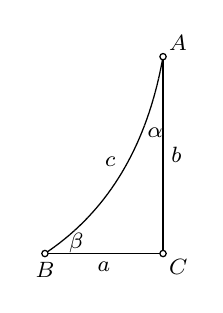
\begin{tikzpicture}
                % \clip (0,0) rectangle (14.000000,10.000000);
                {\footnotesize
                
                % Marking point B by circle
                \draw [line width=0.016cm] (2.000000,2.000000) circle (0.040000);%
                \draw (2.000000,2.000000) node [anchor=north] { $B$ };%
                
                % Marking point C by circle
                \draw [line width=0.016cm] (3.500000,2.000000) circle (0.040000);%
                \draw (3.470000,2.030000) node [anchor=north west] { $C$ };%
                
                % Marking point A by circle
                \draw [line width=0.016cm] (3.500000,4.500000) circle (0.040000);%
                \draw (3.470000,4.470000) node [anchor=south west] { $A$ };%
                
                % Drawing segment B C
                \draw [line width=0.016cm] (2.040000,2.000000) -- (3.460000,2.000000);%
                
                % Drawing segment C A
                \draw [line width=0.016cm] (3.500000,2.040000) -- (3.500000,4.460000);%
                
                % Drawing Bezier curve B X A
                \draw [line width=0.016cm] (2.065972,2.045139) -- (2.033012,2.022587);%
                \draw [line width=0.016cm] (2.130556,2.091667) -- (2.065972,2.045139);%
                \draw [line width=0.016cm] (2.193750,2.139583) -- (2.130556,2.091667);%
                \draw [line width=0.016cm] (2.255556,2.188889) -- (2.193750,2.139583);%
                \draw [line width=0.016cm] (2.315972,2.239583) -- (2.255556,2.188889);%
                \draw [line width=0.016cm] (2.375000,2.291667) -- (2.315972,2.239583);%
                \draw [line width=0.016cm] (2.432639,2.345139) -- (2.375000,2.291667);%
                \draw [line width=0.016cm] (2.488889,2.400000) -- (2.432639,2.345139);%
                \draw [line width=0.016cm] (2.543750,2.456250) -- (2.488889,2.400000);%
                \draw [line width=0.016cm] (2.597222,2.513889) -- (2.543750,2.456250);%
                \draw [line width=0.016cm] (2.649306,2.572917) -- (2.597222,2.513889);%
                \draw [line width=0.016cm] (2.700000,2.633333) -- (2.649306,2.572917);%
                \draw [line width=0.016cm] (2.749306,2.695139) -- (2.700000,2.633333);%
                \draw [line width=0.016cm] (2.797222,2.758333) -- (2.749306,2.695139);%
                \draw [line width=0.016cm] (2.843750,2.822917) -- (2.797222,2.758333);%
                \draw [line width=0.016cm] (2.888889,2.888889) -- (2.843750,2.822917);%
                \draw [line width=0.016cm] (2.932639,2.956250) -- (2.888889,2.888889);%
                \draw [line width=0.016cm] (2.975000,3.025000) -- (2.932639,2.956250);%
                \draw [line width=0.016cm] (3.015972,3.095139) -- (2.975000,3.025000);%
                \draw [line width=0.016cm] (3.055556,3.166667) -- (3.015972,3.095139);%
                \draw [line width=0.016cm] (3.093750,3.239583) -- (3.055556,3.166667);%
                \draw [line width=0.016cm] (3.130556,3.313889) -- (3.093750,3.239583);%
                \draw [line width=0.016cm] (3.165972,3.389583) -- (3.130556,3.313889);%
                \draw [line width=0.016cm] (3.200000,3.466667) -- (3.165972,3.389583);%
                \draw [line width=0.016cm] (3.232639,3.545139) -- (3.200000,3.466667);%
                \draw [line width=0.016cm] (3.263889,3.625000) -- (3.232639,3.545139);%
                \draw [line width=0.016cm] (3.293750,3.706250) -- (3.263889,3.625000);%
                \draw [line width=0.016cm] (3.322222,3.788889) -- (3.293750,3.706250);%
                \draw [line width=0.016cm] (3.349306,3.872917) -- (3.322222,3.788889);%
                \draw [line width=0.016cm] (3.375000,3.958333) -- (3.349306,3.872917);%
                \draw [line width=0.016cm] (3.399306,4.045139) -- (3.375000,3.958333);%
                \draw [line width=0.016cm] (3.422222,4.133333) -- (3.399306,4.045139);%
                \draw [line width=0.016cm] (3.443750,4.222917) -- (3.422222,4.133333);%
                \draw [line width=0.016cm] (3.463889,4.313889) -- (3.443750,4.222917);%
                \draw [line width=0.016cm] (3.482639,4.406250) -- (3.463889,4.313889);%
                \draw [line width=0.016cm] (3.492716,4.460669) -- (3.482639,4.406250);%
                
                % Marking point a
                \draw (2.750000,2.000000) node [anchor=north] { $a$ };%
                
                % Marking point b
                \draw (3.500000,3.250000) node [anchor=west] { $b$ };%
                
                % Marking point c
                \draw (3.000000,3.000000) node [anchor=south east] { $c$ };%
                
                % Marking point \beta
                \draw (2.200000,1.900000) node [anchor=south west] { $\beta$ };%
                
                % Marking point \alpha
                \draw (3.400000,3.700000) node [anchor=north] { $\alpha$ };%
                }
            \end{tikzpicture}
            
            \begin{dokaz}
                \\ Za izračun trigonometričnih funkcij trikotnik prestavimo v posebno lego (z uporabo izometrij).
                \\ \uline{$\sin\alpha$}:
                \\ 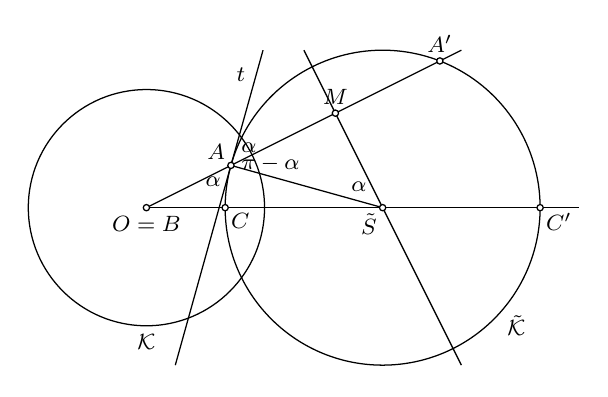
\begin{tikzpicture}
                        % \clip (0,0) rectangle (14.000000,10.000000);
                        {\footnotesize
                        
                        % Marking point O=B by circle
                        \draw [line width=0.016cm] (3.000000,3.000000) circle (0.040000);%
                        \draw (3.000000,3.000000) node [anchor=north] { $O=B$ };%
                        
                        % Marking point C by circle
                        \draw [line width=0.016cm] (4.000000,3.000000) circle (0.040000);%
                        \draw (3.970000,3.030000) node [anchor=north west] { $C$ };%
                        
                        % Marking point \tilde{S} by circle
                        \draw [line width=0.016cm] (6.000000,3.000000) circle (0.040000);%
                        \draw (6.030000,3.030000) node [anchor=north east] { $\tilde{S}$ };%
                        
                        % Drawing circle k
                        \draw [line width=0.016cm] (3.000000,3.000000) circle (1.500000);%
                        
                        % Drawing circle k'
                        \draw [line width=0.016cm] (7.999600,3.039998) -- (7.998782,3.069799) arc (2:67:2.000000 and 2.000000) -- (6.763769,4.848420);%
                        \draw [line width=0.016cm] (6.689240,4.877485) -- (6.684040,4.879385) arc (70:163:2.000000 and 2.000000) -- (4.084468,3.575099);%
                        \draw [line width=0.016cm] (4.063002,3.498037) -- (4.059409,3.483844) arc (166:178:2.000000 and 2.000000) -- (4.000400,3.039998);%
                        \draw [line width=0.016cm] (4.000400,2.960003) -- (4.001218,2.930201) arc (182:358:2.000000 and 2.000000) -- (7.999600,2.960001);%
                        
                        % Marking point C' by circle
                        \draw [line width=0.016cm] (8.000000,3.000000) circle (0.040000);%
                        \draw (7.970000,3.030000) node [anchor=north west] { $C'$ };%
                        
                        % Drawing segment O=B C''
                        \draw [line width=0.016cm] (3.040000,3.000000) -- (3.960000,3.000000);%
                        \draw [line width=0.016cm] (4.040000,3.000000) -- (5.960000,3.000000);%
                        \draw [line width=0.016cm] (6.040000,3.000000) -- (7.960000,3.000000);%
                        \draw [line width=0.016cm] (8.040000,3.000000) -- (8.500000,3.000000);%
                        
                        % Drawing segment O=B X
                        \draw [line width=0.016cm] (7.000000,5.000000) -- (6.762427,4.881214);%
                        \draw [line width=0.016cm] (6.690873,4.845436) -- (5.435777,4.217889);%
                        \draw [line width=0.016cm] (5.364223,4.182111) -- (4.109127,3.554564);%
                        \draw [line width=0.016cm] (4.037573,3.518786) -- (3.035777,3.017889);%
                        
                        % Marking point A by circle
                        \draw [line width=0.016cm] (4.073350,3.536675) circle (0.040000);%
                        \draw (4.103350,3.506675) node [anchor=south east] { $A$ };%
                        
                        % Marking point A' by circle
                        \draw [line width=0.016cm] (6.726650,4.863325) circle (0.040000);%
                        \draw (6.726650,4.863325) node [anchor=south] { $A'$ };%
                        
                        % Drawing line m
                        \draw [line width=0.016cm] (7.000000,1.000000) -- (6.017889,2.964223);%
                        \draw [line width=0.016cm] (5.982111,3.035777) -- (5.417889,4.164223);%
                        \draw [line width=0.016cm] (5.382111,4.235777) -- (5.000000,5.000000);%
                        
                        % Marking point M by circle
                        \draw [line width=0.016cm] (5.400000,4.200000) circle (0.040000);%
                        \draw (5.400000,4.200000) node [anchor=south] { $M$ };%
                        
                        % Drawing segment A \tilde{S}
                        \draw [line width=0.016cm] (4.111883,3.525942) -- (5.961467,3.010734);%
                        
                        % Drawing line t'
                        \draw [line width=0.016cm] (3.366750,1.000000) -- (4.062617,3.498142);%
                        \draw [line width=0.016cm] (4.084084,3.575208) -- (4.480964,5.000000);%
                        
                        % Marking point \alpha
                        \draw (4.050000,3.500000) node [anchor=north east] { $\alpha$ };%
                        
                        % Marking point \alpha
                        \draw (4.100000,3.600000) node [anchor=south west] { $\alpha$ };%
                        
                        % Marking point \alpha
                        \draw (5.900000,3.100000) node [anchor=south east] { $\alpha$ };%
                        
                        % Marking point \pi-\alpha
                        \draw (4.100000,3.550000) node [anchor=west] { $\pi-\alpha$ };%
                        
                        % Marking point t
                        \draw (4.200000,4.500000) node [anchor=south] { $t$ };%
                        
                        % Marking point \tilde{\mathcal{K}}
                        \draw (7.700000,1.500000) node  { $\tilde{\mathcal{K}}$ };%
                        
                        % Marking point \mathcal{K}
                        \draw (3.000000,1.500000) node [anchor=north] { $\mathcal{K}$ };%
                        }
                    \end{tikzpicture}                    
                \\ Naj bo $B=O$ in $C$ na pozitivnem poltraku $x$-osi, $C'$ inverz $C$ v $\mathcal{K}$ in $\tilde{\mathcal{K}}$ krožnica s premerom $CC'$. Nosilka daljice $AC$ je P-premica $\tilde{\mathcal{K}}\cap\mathcal{H}$. Potem inverz $A$ v $\mathcal{K}$ tudi leži na $\tilde{\mathcal{K}}$. Naj bo $t$ tangenta na krožnico $\tilde{\mathcal{K}}$ v točkia $A$. Potem je kot med premicami $t$ in $\overleftrightarrow{OA}$ enak $\alpha$. Naj bo $M$ razpolovišče daljice $AA'$. Potem je $\overleftrightarrow{\tilde{S}M}$ simetrala daljice $AA'$. Ker je $\overleftrightarrow{\tilde{S}A}$ pravokotnica na $t$, sledi, da je $|\angle MA\tilde{S}|=\frac{\pi}{2}-\alpha$ in po tem tudi $|\angle A\tilde{S}M|=\alpha$. V trikotniku $\triangle AM\tilde{S}$ je: $\sin\alpha=\frac{|AM|}{|A\tilde{S}|}=\frac{|AM|}{|C\tilde{S}|}$. Označimo $s=|OA|$ in $q=|OC|$. Potem je $|OA|\cdot|OA'|=1 \Rightarrow |OA'|=\frac{1}{s}$ in $|OC|\cdot|OC'|=1 \Rightarrow |OC'|=\frac{1}{q}$, iz tega pa sledi  $|C\tilde{S}|=\frac{1}{2}|CC'|=\frac{1}{2}\left(|OC'|-|OC|\right)=\frac{1}{2}\left(\frac{1}{q}-q\right)O\frac{1-q^2}{2q}$. Če označimo $a=d(OC)$ dobimo $\sinh{a}=\frac{2q}{1-q^2}$. Podobno velja za $c=d(OA)$: $|AM|=\frac{1}{2}|AA'|=\frac{1-s^2}{2s}$, od tod: $\sinh{c}=\frac{2s}{1-s^2}$. Po vsem skupaj je $\sin\alpha=\frac{|AM|}{|C\tilde{S}|}=\frac{\frac{1}{\sinh{c}}}{\frac{1}{\sinh{a}}}=\frac{\sinh{a}}{\sinh{c}}$.
                \\ \uline{$\cos\alpha$}:
                \\ 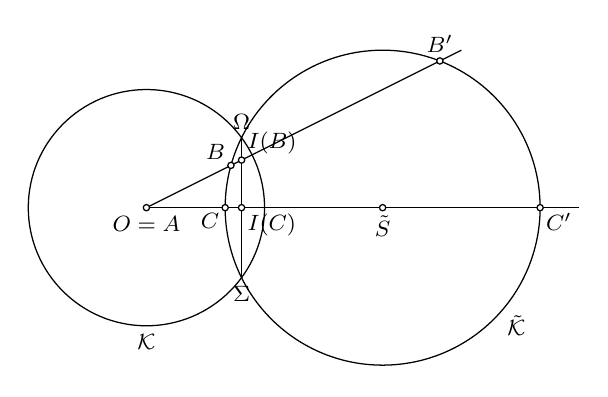
\begin{tikzpicture}
                        % \clip (0,0) rectangle (14.000000,10.000000);
                        {\footnotesize
                        
                        % Marking point O=A by circle
                        \draw [line width=0.016cm] (3.000000,3.000000) circle (0.040000);%
                        \draw (3.000000,3.000000) node [anchor=north] { $O=A$ };%
                        
                        % Marking point C by circle
                        \draw [line width=0.016cm] (4.000000,3.000000) circle (0.040000);%
                        \draw (4.030000,3.030000) node [anchor=north east] { $C$ };%
                        
                        % Marking point \tilde{S} by circle
                        \draw [line width=0.016cm] (6.000000,3.000000) circle (0.040000);%
                        \draw (6.000000,3.000000) node [anchor=north] { $\tilde{S}$ };%
                        
                        % Drawing circle k
                        \draw [line width=0.016cm] (3.000000,3.000000) circle (1.500000);%
                        
                        % Drawing circle k'
                        \draw [line width=0.016cm] (7.999600,3.039998) -- (7.998782,3.069799) arc (2:67:2.000000 and 2.000000) -- (6.763769,4.848420);%
                        \draw [line width=0.016cm] (6.689240,4.877485) -- (6.684040,4.879385) arc (70:163:2.000000 and 2.000000) -- (4.084468,3.575099);%
                        \draw [line width=0.016cm] (4.063002,3.498037) -- (4.059409,3.483844) arc (166:178:2.000000 and 2.000000) -- (4.000400,3.039998);%
                        \draw [line width=0.016cm] (4.000400,2.960003) -- (4.001218,2.930201) arc (182:358:2.000000 and 2.000000) -- (7.999600,2.960001);%
                        
                        % Marking point C' by circle
                        \draw [line width=0.016cm] (8.000000,3.000000) circle (0.040000);%
                        \draw (7.970000,3.030000) node [anchor=north west] { $C'$ };%
                        
                        % Drawing segment O=A C''
                        \draw [line width=0.016cm] (3.040000,3.000000) -- (3.960000,3.000000);%
                        \draw [line width=0.016cm] (4.040000,3.000000) -- (4.168333,3.000000);%
                        \draw [line width=0.016cm] (4.248333,3.000000) -- (5.960000,3.000000);%
                        \draw [line width=0.016cm] (6.040000,3.000000) -- (7.960000,3.000000);%
                        \draw [line width=0.016cm] (8.040000,3.000000) -- (8.500000,3.000000);%
                        
                        % Drawing segment O=A X
                        \draw [line width=0.016cm] (7.000000,5.000000) -- (6.762427,4.881214);%
                        \draw [line width=0.016cm] (6.690873,4.845436) -- (4.244110,3.622055);%
                        \draw [line width=0.016cm] (4.172556,3.586278) -- (4.109127,3.554564);%
                        \draw [line width=0.016cm] (4.037573,3.518786) -- (3.035777,3.017889);%
                        
                        % Marking point B by circle
                        \draw [line width=0.016cm] (4.073350,3.536675) circle (0.040000);%
                        \draw (4.103350,3.506675) node [anchor=south east] { $B$ };%
                        
                        % Marking point B' by circle
                        \draw [line width=0.016cm] (6.726650,4.863325) circle (0.040000);%
                        \draw (6.726650,4.863325) node [anchor=south] { $B'$ };%
                        
                        % Marking point \Omega
                        \draw (4.208333,3.888780) node [anchor=south] { $\Omega$ };%
                        
                        % Marking point \Sigma
                        \draw (4.208333,2.111220) node [anchor=north] { $\Sigma$ };%
                        
                        % Marking point \tilde{\mathcal{K}}
                        \draw (7.700000,1.500000) node  { $\tilde{\mathcal{K}}$ };%
                        
                        % Marking point \mathcal{K}
                        \draw (3.000000,1.500000) node [anchor=north] { $\mathcal{K}$ };%
                        
                        % Drawing segment \Omega \Sigma
                        \draw [line width=0.016cm] (4.208333,3.888780) -- (4.208333,3.644167);%
                        \draw [line width=0.016cm] (4.208333,3.564167) -- (4.208333,3.040000);%
                        \draw [line width=0.016cm] (4.208333,2.960000) -- (4.208333,2.111220);%
                        
                        % Marking point I(B) by circle
                        \draw [line width=0.016cm] (4.208333,3.604167) circle (0.040000);%
                        \draw (4.178333,3.574167) node [anchor=south west] { $I(B)$ };%
                        
                        % Marking point I(C) by circle
                        \draw [line width=0.016cm] (4.208333,3.000000) circle (0.040000);%
                        \draw (4.178333,3.030000) node [anchor=north west] { $I(C)$ };%
                        }
                    \end{tikzpicture}
                \\ Pomagamo si z izomorfizmom med Poincaréjevim krožnim modelom in Beltrami-Kleinovim modelom. Izomorfizem $I$ fiksira premere (ki so premice v obeh modelih), ostale P-premice pa slika na tetive med istimi idealnimi točkami s projekcijo iz središča $O$. Velja: $|OB|=t \Rightarrow |OI(B)|=\frac{2t}{1+t^2}=\tanh{c}$ in $|OC|=s \Rightarrow |OI(C)|=\frac{2s}{1+s^2}=\tanh{b}$. Ker je tirkotnik $\triangle OI(B)I(C)$ pravokoten s pravim kotom pri $I(C)$ ($\overleftrightarrow{CC'}$ je simetrala tetive $\Omega\Sigma$ za $\tilde{\mathcal{K}}$), je potem: $\cos\alpha=\frac{|OI(C)|}{|OI(B)|}=\frac{\tanh{b}}{\tanh{c}}$.
            \end{dokaz}

        \begin{opomba}
            Za majhne trikotnike, $a,b,c\ll 1$, približno velja: $\sinh{a}\doteq a$ in $\tanh{a}\doteq a$. Zato $\sin\alpha\doteq\frac{a}{c}$ in $\cos\alpha\doteq\frac{b}{c}$. Majhni trikotniki so torej približno evklidski.
        \end{opomba}

        \begin{izrek}[Pitagorov izrek v hiperbolični geometriji]
            Naj bo $\triangle ABC$ pravokotni trikotnik s pravim kotom pri $C$ v hiperbolični ravnini. Potem velja $\cosh{c}=\cosh{a}\cdot\cosh{b}$.
        \end{izrek}

            \begin{dokaz}
                \\ Radi bi dokazali, da velja \dashuline{$\cosh{a}=\frac{\cosh{c}}{\cosh{b}}$}.
                \\ Z uporabo ekvivalenc $\tanh{x}=\frac{\sinh{x}}{\cosh{x}}$ in $\cosh^2{x}-\sinh^2{x}=1$, pridemo do enačbe:
                \begin{align*}
                    \cosh{a}&=\sqrt{1+\sinh^2{a}}= \\
                            &=\sqrt{1+(\sin{\alpha}\cdot\sinh{c})^2}= \\
                            &=\sqrt{1++\sin^2{\alpha}\cdot\sinh^2{c}}= \\
                            &=\sqrt{1+\sinh^2{c}-\sin^2{\alpha}\cdot\sinh^2{c}}= \\
                            &=\sqrt{\cosh^2{c}-\frac{\sinh^2{b}\cdot\cosh^2{c}}{\cosh^2{b}}}= \\
                            &=\cosh{c}\cdot\sqrt{1-\frac{\sinh^2{b}}{\cosh^2{b}}}= \\
                            &=\cosh{c}\cdot\sqrt{\frac{\cosh^2{b}-\sinh^2{b}}{\cosh^2{b}}}= \\
                            &=\frac{\cosh{c}}{\cosh{b}}
                \end{align*}
            \end{dokaz}

        \begin{izrek}[sinusni izrek v hiperbolični geometriji]
            Naj bo $\triangle ABC$ trikotnik v hiperbolični ravnini. Potem velja $\frac{\sinh{a}}{\sin{\alpha}}=\frac{\sinh{b}}{\sin{\beta}}=\frac{\sinh{c}}{\sin{\gamma}}$.
        \end{izrek}

            \begin{dokaz}
                \\ Recimo, da je $\triangle ABC$  ostrokotni trikotnik. Dokažimo: $\frac{\sinh{a}}{\sin{\alpha}}=\frac{\sinh{b}}{\sin{\beta}}$. Dokaz ostalih enakosti je podoben.
                \\ Trikotniku kostruiramo višino $h$ na stranico $c$. Tako dobimo dva pravokotna trikotnika $\triangle ADC$ in $\triangle BDC$ s pravim kotom pri $D$. Velja: $\sin{\alpha}=\frac{\sinh{h}}{\sinh{b}}$ in $\sin{\beta}=\frac{\sinh{h}}{\sinh{a}}$. Od tod pa sledi $\frac{\sinh{a}}{\sin{\alpha}}=\frac{\sinh{b}}{\sin{\beta}}$.
            \end{dokaz}

        \begin{izrek}[kosinusni izrek v hiperbolični geometriji]
            Naj bo $\triangle ABC$ trikotnik v hiperbolični ravnini. Potem velja $\cosh{c}=\cosh{a}\cdot\cosh{b}-\sinh{a}\cdot\sinh{b}\cdot\cos{\gamma}$.
        \end{izrek}

            \begin{dokaz}
                \\ Recimo, da je $\triangle ABC$ ostrokotni trikotnik. (Za topokotni trikotnik velja podobno.)
                \\ Trikotniku kostruiramo višino $h$ na stranico $a$ in tako dobimo pravokotna trikotnika $\triangle ADB$ in $\triangle ADC$ s pravim kotom pri $D$. V prvem velja: $\cosh{c}=\cosh{h}\cdot\cosh{x}$, kjer je $x=|DB|$; v drugem pa: $\cosh{b}=\cosh{h}\cdot\cosh{y}$, kjer je $y=|CD|$. Od tod sledi, ob upoštevanju $\cos{\gamma}=\frac{\tanh{y}}{\tanh{b}}=\frac{\sinh{y}\cdot\cosh{b}}{\cosh{y}\cdot\sinh{b}}$, da je: 
                    \begin{align*}
                        \cosh{c}&=\frac{\cosh{b}}{\cosh{y}}\cosh{x}= \\
                                &=\frac{\sinh{b}}{\sinh{y}}\cosh{x}\cdot\cos{\gamma}= \\
                                &=\frac{\cosh{b}}{\cosh{y}}\cosh{a-y}= \\
                                &=\frac{\cosh{b}}{\cosh{y}}(\cosh{a}\cdot\cosh{y}-\sinh{a}\cdot\sinh{y})= \\
                                &=\cosh{b}\cdot\cosh{a}-\frac{\cosh{b}\cdot\sinh{a}\cdot\sinh{y}}{\cosh{y}}= \\
                                &=\cosh{a}\cdot\cosh{b}-\sinh{a}\cdot\sinh{b}\cdot\cos{\gamma}
                    \end{align*}
            \end{dokaz}

